%% Undergraduate thesis paper
%%
%% M E M E R A T O R
%%
%% Author: AlOrozco53
%% Advisor: ivanvladimir
%% Version: 0.0
\documentclass[letter]{book}
\usepackage[utf8]{inputenc}
\usepackage[T1]{fontenc}
\usepackage{graphicx}
\usepackage[spanish]{babel}
\usepackage[style=trad-abbrv]{biblatex}
\usepackage{quotchap}

\addbibresource{bibliography.bib}
\setlength{\parindent}{4em}
\setlength{\parskip}{1em}
\newcommand{\twelveptsize}{%
  \fontsize{12}{15}\selectfont}

\graphicspath{{img/}} %% image directory

\begin{document}

\thispagestyle{empty}

\frontmatter

\begin{titlepage}
  \begin{minipage}{.3\textwidth}
    \flushleft
    \center{
\includegraphics[scale=.09]{unam.pdf}}
    \vspace{20pt}
    \center{
      \rule{.5pt}{.6\textheight}
      \hspace{7pt}
      \rule{2pt}{.6\textheight}
      \hspace{7pt}
      \rule{.5pt}{.6\textheight}
    }\\
    \center{
\includegraphics[scale=.22]{ciencias.pdf}}
  \end{minipage}
  \begin{minipage}{.7\textwidth}
    \flushright
    \center{
      \center{
        \LARGE{U}\large{NIVERSIDAD} \LARGE{N}\large{ACIONAL}
        \LARGE{A}\large{UTÓNOMA} \\[10pt]
        \large{DE}
        \LARGE{M}\large{ÉXICO}
      }\\
      \rule{\textwidth}{2pt}
      \\
      \hrulefill\\[1cm]
      \LARGE{F}\large{ACULTAD DE } \LARGE{C}\large{IENCIAS}\\[2cm]
      \large{
        Generación automática de memes de Internet a través de una red neuronal profunda  }\\[2cm]
      \huge{
        T \hspace{1cm} E \hspace{1cm} S \hspace{1cm} I \hspace{1cm} S  }\\[1cm]
      \large{QUE PARA OBTENER EL TÍTULO DE:}\\[1cm]
      \large{
        Licenciado en Ciencias de la Computación  }\\[1cm]
      \large{PRESENTA:}\\[1cm]
      \large{
        Albert Manuel Orozco Camacho  }\\[1cm]
      \large{
        TUTOR  }\\[1cm]
      \large{
        Dr. Ivan Vladimir Meza Ruiz  }
    }
  \end{minipage}
\end{titlepage}

\tableofcontents

\mainmatter

\twelveptsize

\begin{savequote}[45mm]
  When you plant a fertile meme in my mind you literally parasitize my brain,\
  turning it into a vehicle for the meme's propagation in just the way that a\
  virus may parasitize the genetic mechanism of a host cell.
  \qauthor{Richard Dawkins \cite{dawkins2006}}
\end{savequote}

\chapter{Introducción}

\noindent
El siglo XXI ha traido consigo una transformación radical en las formas de comunicación\
entre personas. Hoy en día, el uso de redes sociales \emph{democratiza} el acceso\
a la información más relevante ocurriendo en tiempo real, sin tener que esperar a que un medio\
masivo publique una noticia sobre ello. Cualquier persona con una cuenta de \textit{Twitter} puede\
tomar una fotografía, subirla a la \textit{web} y etiquetarla de la manera en que más le convenga (mediante\
\textit{hashtags}, por ejemplo). Dependiendo de muchos factores, incluyendo el alcance del\
\textit{tuit} y el número de seguidores de la cuenta de Twitter, es posible que la imagen se vuelva\
más popular de lo que una nota publicada por algún periodista serio pueda alcanzar.\par
Este fenómeno también se explica por las intenciones que llevan a la gente a interactuar dentro de\
las redes sociales. Al usuario se le da la libertad de hacer que el contenido de su \textit{timeline (TL)}\
sea tan ocioso, o tan serio, como éste quiera, siguiendo en el caso de Twitter. Cuando un tuit acompañado\
de una imagen se vuelve \emph{viral}, surge un fenómeno de propagación en el cual el poder del\
\textit{tuitero} permite re-etiquetar la imagen sin perder la esencia de la idea original transimitida\
por la misma.\par
En general, este fenómeno no es exclusivo de Twitter y ha ocurrido en Internet desde que la comunicación\
entre personas se efectuaba exclusivamente por medio de correos electrónicos. Para englobar a las diversas\
maneras en las que se viraliza cierta infomación en la web en un solo concepto, se ha popularizado el\
término \emph{\textbf{meme (de Internet)}}, el cual pretende \emph{discretizar} la información cultural\
en unidades capaces de pasar de persona a persona, gradualmente escalar en un fenómeno social compartido\
e incluso \emph{evolucionar} \cite{shifman2014}.\par
Paralelamente, el constante incremento en el uso de redes sociales genera un cúmulo de datos esparcidos\
por el Internet. De acuerdo al un estudio descrito en \cite{website:smartinsights} y publicado en 2016,\
el $46\%$ de la población mundial son usuarios de Internet y el $31\%$ son usuarios activos de alguna red social.\
Además, durante 2015 se produjo un aumento de usuarios equivalente a $10\%$ en los dos rubros descritos anteriormente.\
Consecuencia de esto es que a diario, el intercambio de información favorece en la riqueza y complejidad\
de nuevas ideas que se acumulan en grandes servidores pero cuya relevancia está empezando a ser explorada.\par
Dentro de la rama de las ciencias de la computación, conocida como \textbf{inteligencia artificial}, el\
\textbf{aprendizaje automático} (\emph{machine learning} en inglés) propone técnicas capaces de lograr que, a partir\
de grandes cantidades de datos, un sistema de cómputo revele información oculta para muchos seres humanos.\
El auge del subconjunto de \emph{algoritmos de aprendizaje} automático conocido como\
\textbf{aprendizaje profundo} (\emph{deep learning} en inglés), trae consigo un importante adelanto\
en el desempeño de computadoras al realizar habilidades humanas. Dos ejemplos significativos incluye el reconocimiento\
de imágenes y rostros mediante visión computacional y la generación automática de texto coherente en algún idioma.\par
Motivado por lo establecido en los párrafos anteriores, en el presente trabajo se explorarán dos modelos de\
aprendizaje profundo para entrenar, identificar y, finalmente, etiquetar memes de Internet. Se considerará únicamente\
el caso de una imagen (la cual, en el la mayoría de los casos, incluye a un solo personaje) y una \emph{leyenda} asociada.\
Por lo tanto, se presentará un método para hacer que la computadora aprenda al personaje dentro del meme y la información\
textual que transmite; posteriormente se experimentará etiquetando memes no antes vistos por dicha computadora.

\section{Memes de Internet y \emph{memética}}

\noindent
El término \emph{meme} fue acuñado por el biólogo Richard Dawkins en su libro \emph{``The Selfish Gene''}\
de 1976. Mediante una analogía con el papel del \emph{gen} en la evolución darwiniana, Dawkins\
propuso una teoría cultural en la cual el meme es visto como la unidad que se propaga por generaciones\
y sobrevive mediante un proceso semejante a la selección natural. Dawkins conjeturó que la teoría de la evolución\
de Darwin es una instancia particular de un proceso que se puede encontrar en otras áreas; en particular,\
es suficiente que cualquier concepto que incorpore las propiedades de \emph{longevidad}, \emph{fecundidad} y\
\emph{fidelidad de copias} para que éste tenga un comportamiento evolutivo a través del tiempo \cite{distin2005}.\par
Hoy en día, se le conoce como \emph{meme} principalmente al objeto proveniente de Internet y que incorpora,\
en el mayor de los casos, una imagen y una leyenda que cuenta algo sobre la imagen. Es importante recalcar\
el aspecto humorístico, muchas veces incluso irónico, que caracteriza al meme de la actualidad ya que ello\
contribuye a la difusión de los mismos por la web. Sin embargo, es el diseño \emph{centrado al usuario} característico\
de la llamada \emph{Web 2.0} lo que mayormente facilita la propagación de memes.\par
Dentro de esta estructura tecnológica, las tres propiedades adscritas por Dawkins a cualquier objeto evolutivo se\
satisfacen para los memes: la digitalización permite una transmisión casi sin interferencias (fidelidad de copias),\
el número de copias compartidas en una unidad de tiempo es incremental -- dada la facilidad de compartir información\
``de nodo a nodo'' -- (fecundidad) y el aumento en la longevidad de la información es respaldado por la capacidad de\
almacenamiento indefinido en los servidores de la web. \href{http://www.reddit.com}{\texttt{Reddit.com}} es uno\
de los sitios web con mayor flujo y contenido de memes; su eslogan \emph{``the front page of the Internet''}\
resume la importancia cultural que el alcance de su contenido modifica las formas de obtener y discutir información\
de cualquier índole. Lo que Dawkins no se imaginó en los años 70's es que el meme se convertiría en la mejor\
manera de encapsular los aspectos más fundamentales de Internet \cite{shifman2014}.

\begin{figure}
  \centering
  
\includegraphics[width=0.5\textwidth]{success_kid}
  \caption{Clásico ejemplo de un personaje \emph{memificado} junto con una de sus
    leyendas (descripciones). Tomado de \href{http://www.memegenerator.net}{MemeGenerator.net}
    \cite{website:memegenerator:kid}.
  }
\end{figure}

La trascendencia del concepto de Dawkins provocó el surgimiento de la \emph{memética}, la disciplina\
sociobiológica que extrapola el concepto de evolución de la teoría de Darwin para colocar al\
meme como instrumento de supervivencia, un \emph{replicador}. Originalmente, Dawkins sugirió como\
ejemplos de memes a frases pegadizas, tonos de audio, modas, habilidades o simplemente ideas.\
Más aún, según Dawkins el meme es una ``unidad de información que reside en un cerebro'' \cite{dawkins2006},\
una afirmación que sugiere la relevancia que el alcance de las redes sociales tiene en la población\
actual, incluso mayor a la que otros medios de comunicación -- como la televisión o la radio -- alcanzaron\
desde su concepción.

\section{Un esbozo sobre las redes neuronales profundas}

\section{Objetivos de la tesis}

\chapter{Marco teórico}

\noindent
\emph{¿Cómo es que la mente humana llega a etiquetar una imagen?} A pesar de que las\
técnicas y algoritmos que se presentarán en esta tesis están diseñados para su implementación en\
una computadora, la filosofía que hay detrás de ellos se inspira en la del funcionamiento del cerebro\
humano. Antes de la conceptualización de la \textbf{inteligencia artificial} (IA) como disciplina científica,\
diversos pensadores como Ramón Llull, Thomas Hobbes y Leonardo da Vinci, ya habían propuesto la idea\
de \emph{mecanizar} el razonamiento mediante una máquina apta para realizar cálculos numéricos. \cite{russell2010}\par
En 1642, Blaise Pascal construyó la primera máquina capaz de realizar cálulos (sumas y restas): la \emph{Pascalina}.\
Las capacidades de ésta última fueron superadas por la máquina de Gottfried Wilhelm Leibniz,\
la cual, además de sumar y restar, también podía multiplicar y sacar raíces. La idea central detrás\
de todo lo anterior radicaba en aceptar la existencia de un conjunto de \emph{reglas lógicas} que\
gobiernan a la mente y al pensamiento. Esto arrancó cuando Aristóteles formuló una serie de\
silogismos capaces de generar conclusiones automáticas a partir de premisas iniciales. Sin embargo,\
la \emph{tradición lógica} de la IA no pudo superar dos obstáculos principales: pasar de\
conocimiento \emph{informal} a términos fomales y resolver un problema fuera de la teoría.\cite{russell2010}.\par

\section{Aprendizaje automático}

\noindent
En la literatura más tradicional de IA, se acostumbra motivar y guiar la teoría por medio de\
las capacidades y limitaciones de un \textbf{agente} (racional). Esto es una abstracción de un ente real,\
capaz de percibir información de su ambiente, procesarla y tomar decisiones. El agente será\
equipado del conocimiento necesario para decidir la mejor opción según lo que exista en su entorno.\par
La arquitectura interna del agente se compone de una máquina finita de \emph{estados} (con sus variantes),\
cuyas transiciones están determinadas por \emph{reglas de interpretación}. Cada vez que un agente\
cambia de estado, se produce una \emph{acción}. La naturaleza de esta estructura nos lleva a reducir\
muchos de los problemas de la IA en búsquedas, en las cuales el agente puede o no saber \emph{a priori}\
el conjunto de posibles resultados que puede encontrar.\par
Computacionalmente hablando, el espacio de búsqueda de varios problemas interesantes en IA se vuelve\
bastante intratable, por lo que no es posible simplemente codificar todos los posibles escenarios\
dentro de la \emph{base de conocimientos} de un agente. El camino hacia la solución a este problema\
comienza con dos observaciones:
\begin{itemize}
\item un agente puede (y debe) ser capaz de manejar la incertidumbre de su entorno dependiendo\
  de la verosimilitud de un evento;
\item el cerebro humano pasa mucho tiempo adquiriendo conocimiento a través de experiencias\
  que previamente \emph{aprendió}, por ende, no es descabellado enseñar a un agente a que\
  automáticamente se genere una descripción de su entorno.
\end{itemize}

\begin{figure}[H]
  \centering
  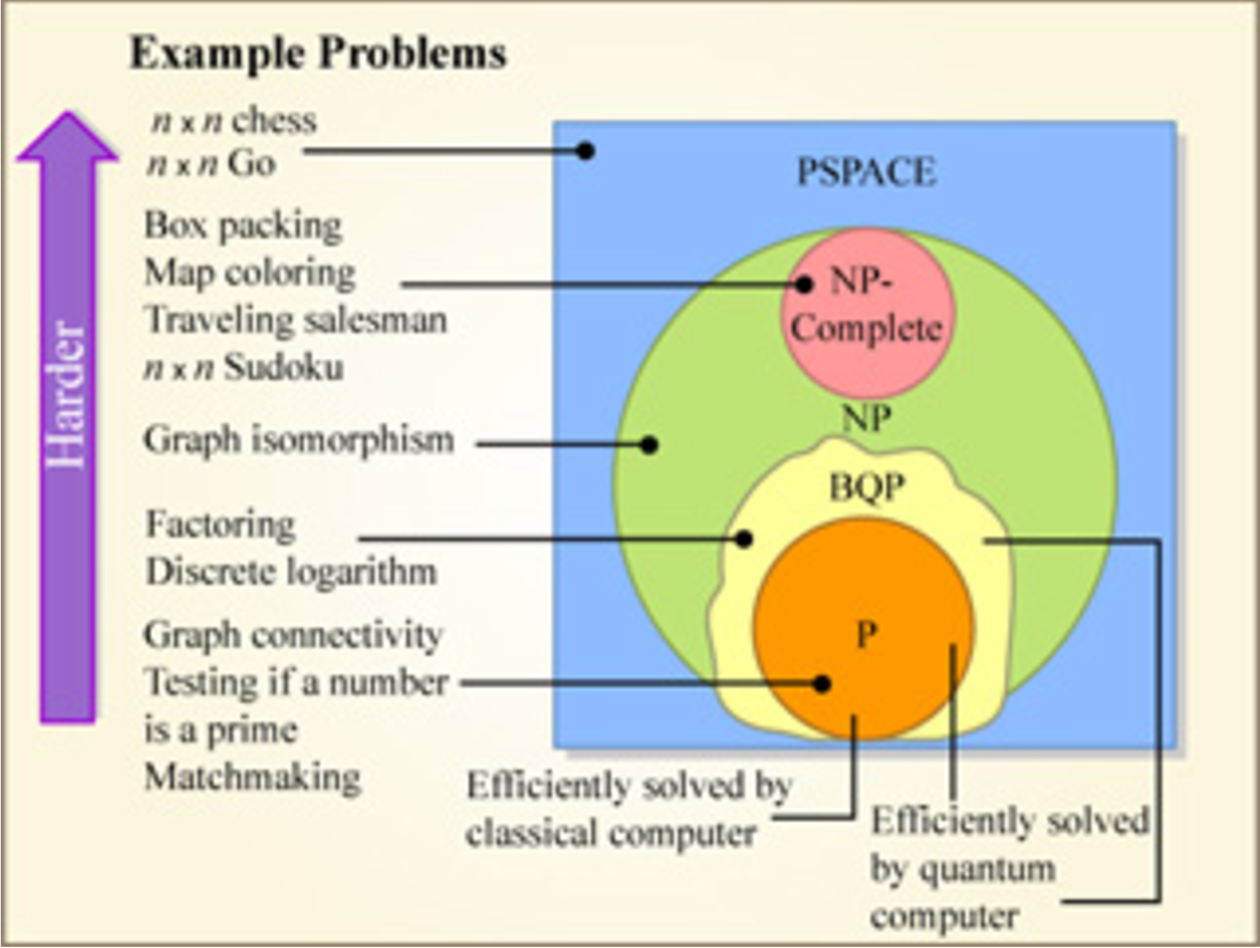
\includegraphics[width=\textwidth]{ai_complexity}
  \caption{La complejidad de algunos problemas en computación. En particular, el \emph{ajedrez}
    y el \emph{go} han sido dos juegos de mesa de gran interés en inteligencia artificial. La historia
    relata que en 1997 la computadora \emph{Deep Blue} de IBM fue capaz de vencer al gran campeón Garry Kaspárov.
    No obstante, su requerimiento de guardar una cantidad \emph{polinomial} de memoria, hacen que en la
    actualidad se estudien modelos capaces de aprender a jugar tanto ajedrez como go, a partir de la observación de partidas.
    (Tomado de (\url{https://ocw.mit.edu/courses/electrical-engineering-and-computer-science/6-845-quantum-complexity-theory-fall-2010/}))}
\end{figure}


El \textbf{aprendizaje automático} (\emph{machine learning} en inglés) es la rama de la IA que trata con algoritmos que son capaces\
de tratar con información estructuralmente incierta (o ruidosa) y generar modelos internos para\
la toma de decisiones. Un agente equipado con la habilidad de aprender automáticamente\
se beneficia de grandes cantidades de ejemplos de un problema, pues su objetivo ahora es\
llegar al mejor modelo, estadísticamente hablando.

\subsection{Las diferentes formas con las que una máquina aprende}

\noindent
La mayoría de los retos computacionales tienen como solución un programa determinístico. Su objetivo\
radica en que dada una entrada $\vec{x}$, el programador diseña en su mente un algoritmo $h$ que calcule\
la salida deseada $z = h(\vec{x})$.\par
En cambio para estimar $z$, en aprendizaje automático, el programador o científico de datos propone un \emph{modelo} $h$\
que sea \emph{entrenado} con respecto a una función objetivo (o de error) $J$, optimizando así, una posible\
solución $\hat{z}$. Todo esto se hace teniendo en cuenta un conjunto de \emph{parámetros} del modelo y\
un conjunto de datos muestrales $\mathcal{D}$.

\begin{figure}[h]
  \centering
  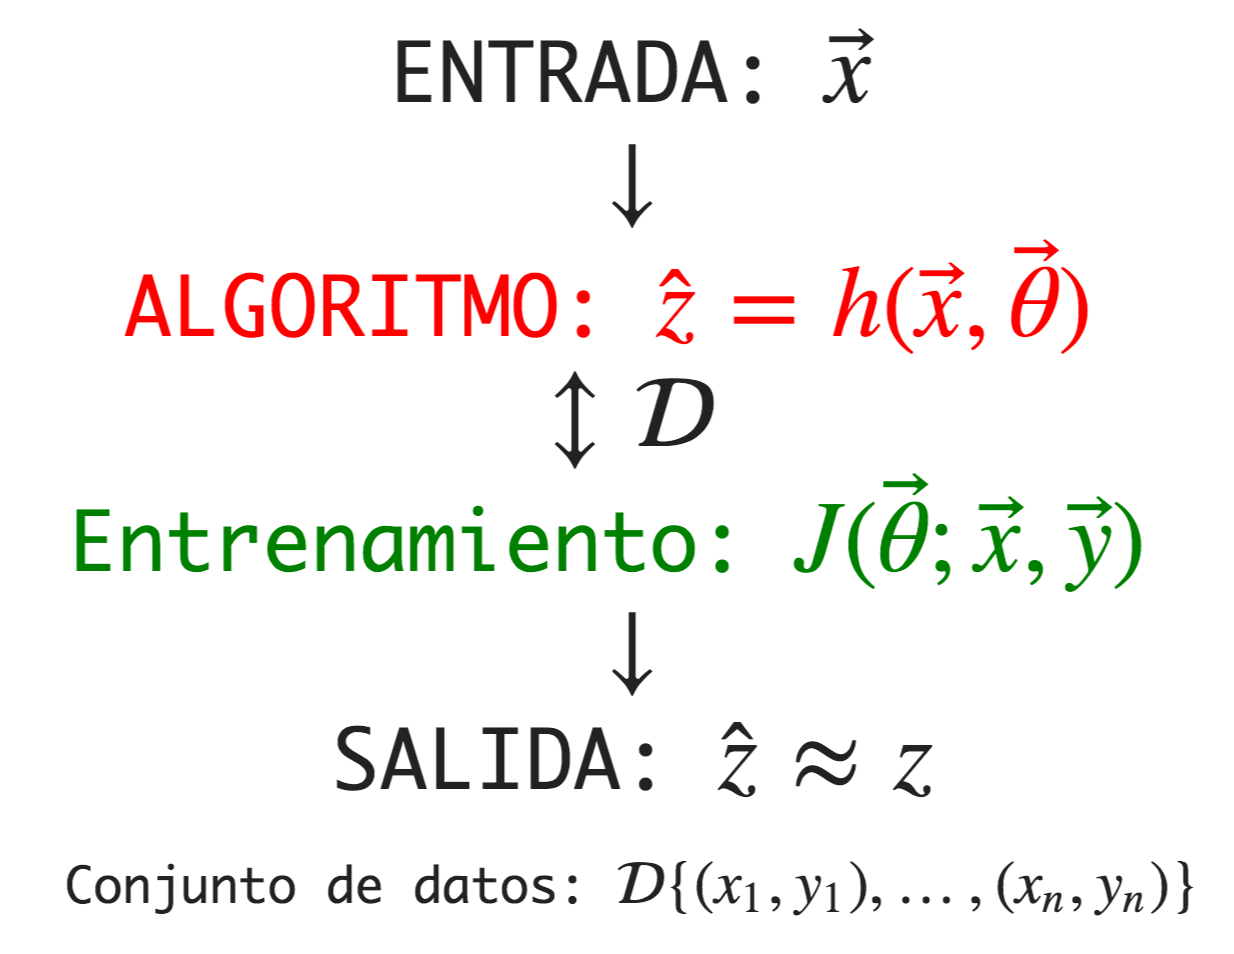
\includegraphics[width=\textwidth]{ml}
  \caption{Las tres fases del aprendizaje automático supervisado.
    (Elaboración propia.)}
\end{figure}

Las maneras de hacer aprendizaje automático dependen de cómo está constituido el conjunto de datos con el\
que se trabaja. En \textbf{aprendizaje supervisado}, se modelan fenómenos a través de muchos ejemplos\
\emph{etiquetados}, es decir, el conjunto de datos puede ser visto como
\begin{equation}
  \mathcal{D} = \{(x_1, y_1),\ldots,(x_n, y_n)\}.
\end{equation}
En este caso, se dice que $\mathcal{D}$ contiene $n$ ejemplos etiquetados: a $\vec{x}$ y a $\vec{y}$ se\
les puede ver como instancias de posibles entradas y salidas del problema $z$, respectivamente. Normalmente,\
$\vec{x}$ se compone de valores numéricos que que fungen como \emph{características} distintivas de la entrada.
El vector $\vec{y}$ puede contener valores de un conjunto discreto (categorías) o continuo.\par
Formalmente, suponiendo que $x_i \in \mathbf{X}$ e $y_i \in \mathbf{Y}$ un algoritmo $h$\
de aprendizaje automático tiene la forma
\begin{equation}
  h: \mathbf{X} \longrightarrow \mathbf{Y}.
\end{equation}
Si $\mathbf{Y}$ es un conjunto finito, entonces decimos que el problema es de \textbf{clasificación}, mientras\
que si es infinito (y denso) es de \textbf{regresión}.\par
En la presente tesis, se trabajará únicamente con aprendizaje supervisado, pues cada uno de los memes de\
muestra ($\mathbf{X}$), está etiquetado con una o varias leyendas ($Y$). El reto consiste en construir un\
modelo que sea capaz de capturar las características más importantes de la imagen y que las asocie a un\
\emph{modelo de lenguaje}. Todo esto será profundizado más adelante.\par
Para terminar con la teoría general de aprendizaje automático, vale la pena destacar que es posible\
realizar \textbf{aprendizaje no supervisado}. Esto se logra mediante un conjunto de datos que carece\
de salidas $\mathbf{Y}$; el objetivo de un agente será desvelar los patrones que comparten las características\
dadas, es decir, aprender a agrupar los datos mediante el uso de similitudes estadísticas.\
\textbf{Aprendizaje por refuerzo} es otra manera de hacer aprendizaje automático y se basa en\
un entrenamiento en el que el ajente debe de maximizar un puntaje debido a una retroalimentación\
dada por sus acciones. Esto último va más allá de los objetivos de esta tesis.

\section{Aproximando funciones con neuronas}

\noindent
En computación, la palabra \emph{aprendizaje} es sinónimo de ``minimización de\
errores'', lo que lleva a cuestionarnos la existencia de una conexión entre\
este fenómeno estadístico con las maneras que, naturalmente, posee el cuerpo humano\
para comprender su medio ambiente. Concretamente, la tarea que tiene el computólogo\
ante sí consiste en transformar los problemas de aprendizaje automático en\
equivalentes compatibles con el funcionamiento del sistema nervioso humano. Dadas,\
las evidencias empíricas sobre el buen desempeño del cerebro humano en su cotidianidad,\
nos inspiramos en el comportamiento biológico del mismo para construir arquitecturas\
cuyo objetivo será el de aproximar funciones complejas, creando un novedoso paradigma de cómputo.\par
Con el fin de ilustrar al buen \emph{performance} del cerebro humano, consideremos a las\
habilidades de reconocimiento perceptivo. Mientras una persona tarda de $100$ a $200$ $ms$\
en detectar un rostro familiar, una computadora con suficiente poder dura mucho más.\cite{haykin2009}\
En contraste, se sabe que individualmente, una neurona es mucho más lenta que una\
compuerta lógica: mientras que ésta última tarda pocos nanosegundos en \emph{conmutar},\
a la primera mencionada le puede tomar varios milisegundos en reaccionar a un estímulo.

\subsection{Inspiración a partir de la biología}

\noindent
El sistema nervioso es una red \emph{paralela} y \emph{auto-organizada}. $86$ mil\
millones de neuronas (aproximadamente) \cite{website:nature:scitable} conforman una arquitectura que\
funciona a través de la emisión de pulsos eléctricos y la reacción ante ellos. Dos neuronas\
están conectadas entre sí por medio de estructuras conocidas como \emph{sinapsis},\
a través de las cuales se transmiten señales eléctricas y químicas.\par
El cerebro es, además, un órgano que se adapta a las condiciones de su ambiente.\
Evidencia de ello es la creación de conexiones sinápticas entre neuronas (previamente\
desconectadas) y la modificación del mecanismo de las sinapsis existentes. Una vez que una\
neurona haya emitido una señal eléctrica, las adyacentes reciben la \emph{``información''}\
por medio de canales de transimisión llamados \emph{dendritas}. Estos impulsos son llevados\
hasta el \emph{cuerpo} de la neurona para su procesamiento y, posteriormente, una reacción\
es transmitida a través del \emph{axón} de la célula. Los organelos mencionados anteriormente\
constituyen las principales partes de la neurona que habrán de servir como estructuras\
fundamentales de las arquitecturas de aprendizaje a presentar en las siguientes secciones.\cite{rojas1996}

\begin{figure}[h]
  \centering
  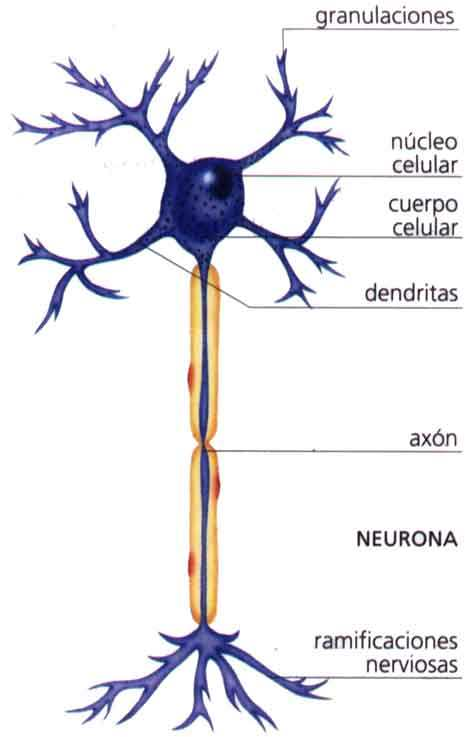
\includegraphics[width=0.6\textwidth]{neurona}
  \caption{Ilustración de las partes más importantes de una neurona humana.
    (Tomado de (\url{https://psi121f.wordpress.com/2016/07/03/la-estructura-de-la-neurona-2/}))}
\end{figure}


\subsection{El modelo de cómputo neuronal}

\noindent
Dadas varias entradas eléctricas, una neurona deberá de ajustar su reacción de manera proporcional\
a la intensidad de las dichas señales. Para formalizar el comportamiento de una neurona en términos\
matemáticos (y, por ende, computacionales), es imprescindible caracterizar las reglas que sigue una neurona\
para componer sus señales de entrada y manejarlas ``globalmente'' mediante una función. Cabe destacar\
que, por simplicidad y elegancia de los modelos a estudiar, resulta importante conocer la \emph{sincronía}\
de la transmisión de información así como la presencia o ausencia de ciclos o bucles. Todo esto se puede\
englobar en un conjunto de características topológicas y algorítmicas que constituyen a una \emph{red neuronal artificial}\
(ANN, por sus siglas en inglés; en adelante, abreviaremos ANN con NN).\par
Con respecto a la representación interna del conocimiento de una NN, estamos ante un conjunto de modelos\
que buscarán modelar la información de manera \emph{asociativa}; análogamente al cerebro humano. Por ende,\
se requieren modelos que \emph{relacionen} clasificaciones de objetos similares con representaciones internas\
similares. Con el fin de asegurarnos de ello, presentaremos más adelante una completa sección\
acerca de métodos para medir similitud. Una consecuencia importante de esto es que,\
de manera contraria, si se desea que dos objetos sean distintamente clasificados,\
entonces se les deben de dar dos representaciones totalmente diferentes.\par
Independientemente de la tarea que se desea aprender, siempre existirá alguna característica cuya importancia\
define el veredicto de la NN. Una forma de respaldar este hecho consiste en dedicar un gran\
número de neuronas a la identificación de dicha característica. Con ello, se aumenta la\
precisión de la NN en su toma de decisiones, contrastando con la existencia de neuronas defectuosas.\par
Finalmente, la existencia de un \emph{zoológico de redes neuronales} se justifica con la tendencia\
que se sigue a diseñar modelos específicos para ciertas tareas. Si se sabe información \textit{a priori}\
sobre los datos a procesar, es mejor integrarlas en el diseño de la arquitectura a dejar que ésta\
los aprenda durante el entrenamiento. Después de todo, en el cuerpo humano existen una gran cantidad\
de estructuras neuronales especializadas para funciones como visión y audición, muy distintas a otras\
presentes en el cerebro.

\subsection{El perceptrón de Rosenblatt}

\noindent
El contenido de este apartado se basa principalmente de \cite{haykin2009} y \cite{rojas1996}.\par
La idea de cómputo a través de redes neuronales fue tan trascendente desde su concepción, que, en 1943,\
McCulloch y Pitts la incluyeron en el mismo artículo que introdujo a los sistemas de transición con un número\
finito de estados \cite{mcculloch:pitts}. Sin embargo, fue Rosenblatt, en 1958, quien propuso el primer modelo de aprendizaje supervisado para una NN.\
El perceptrón es la red neuronal más simple y, muchas veces, será uno de los bloques básicos de arquitecturas\
más complejas. La intuición matemática detrás de su estructura consiste en \emph{separar linealmente} las entradas dadas en\
dos clases, lo cual se logra mediante un aprendizaje que va ajustando pesos de acuerdo a las salidas esperadas.\par

\begin{figure}[h]
  \centering
  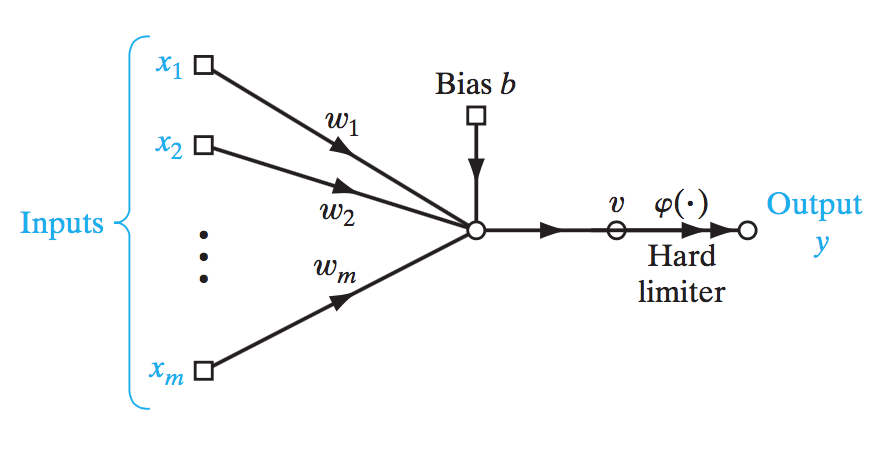
\includegraphics[width=\textwidth]{perceptron}
  \caption{El perceptrón de Rosenblatt es un modelo gráfico cuya salida depende de las contribuciones
    lineales de cada una de las entradas, de un sesgo y de una función no lineal de activación.
    (Tomado de \cite{haykin2009})}
  \label{perceptron-fig}
\end{figure}


De acuerdo a la Figura \ref{perceptron-fig}, el perceptrón opera de la siguiente manera: dados los valores\
de entrada $x_1, x_2,\ldots, x_m$ y los pesos $w_1, w_2,\ldots, w_m$,
\begin{itemize}
\item se calcula una suma ponderada con los $m$ pesos (\emph{sinápticos}) del modelo,
\item a la suma anterior, se le añade un valor de \emph{``tendencia''} conocido como \emph{sesgo}\
  (\emph{bias} en inglés); formalmente:
  \begin{equation}
    v = b + \sum_{i=1}^{m} w_ix_i
  \end{equation}
\item finalmente, la salida del perceptrón se calcula aplicando una función \emph{de activación} a $v$:
    \begin{equation}
      y = \Phi(v).
    \end{equation}
\end{itemize}

La función de activación juega el papel directo de clasificador: su salida debe decidir si la entrada\
pertenece, o no, a cierta clase. De ahí que en la mayoría de los casos, se trata de una función cuya imagen\
es $\{0,1\}$ o $\{-1,1\}$. Por otra parte, dado que estamos definiendo al perceptrón con operaciones\
aritméticas como sumas y productos, cabe recalcar que las entradas deben ser una \emph{abstracción numérica}\
del elemento del entorno a clasificar; muchas veces ésta se compone de un vector de valores reales. Ello implica\
la existencia de un \emph{umbral} $U$ (\emph{threshold} en inglés) que divida los posibles valores de $v$\
en dos, permitiendo su clasificación binaria. A continuación, se define la \emph{función escalón}, valuada\
en $\{-1,1\}$ (una posible función de activación):
\begin{equation}
  \Phi(v) =
  \begin{cases}
    1 & \text{si } v > U\\
    -1 & \text{en otro caso}
  \end{cases}
\end{equation}
Geométricamente, el perceptrón genera un \emph{hiperplano} que, con los pesos adecuados logrará dividir\
las entradas de manera que cada entrada correspondiente a una cierta clase quede dentro de \emph{una y sólo una}\
partición del espacio multidimiensional en cuestión.\par
El hecho de que estamos usando funciones de activación valuadas de manera binaria nos invita a explorar el\
cómputo \emph{neuronal} de las diversas funciones lógicas. Como ejemplo, está la clasificación de\
la función \verb+OR+ en la Figura \ref{or-fig}. En este caso, se tienen entradas de dos dimensiones, por lo que es\
posible visualizarlas gráficamente; en la práctica, se trabaja con un gran número de dimensiones, de lo cual\
se deduce la importancia de tomarán algunos métodos de reducción dimensional para el éxito de los algoritmos\
de entrenamiento de modelos más complejos.\par

\begin{figure}[h]
  \centering
  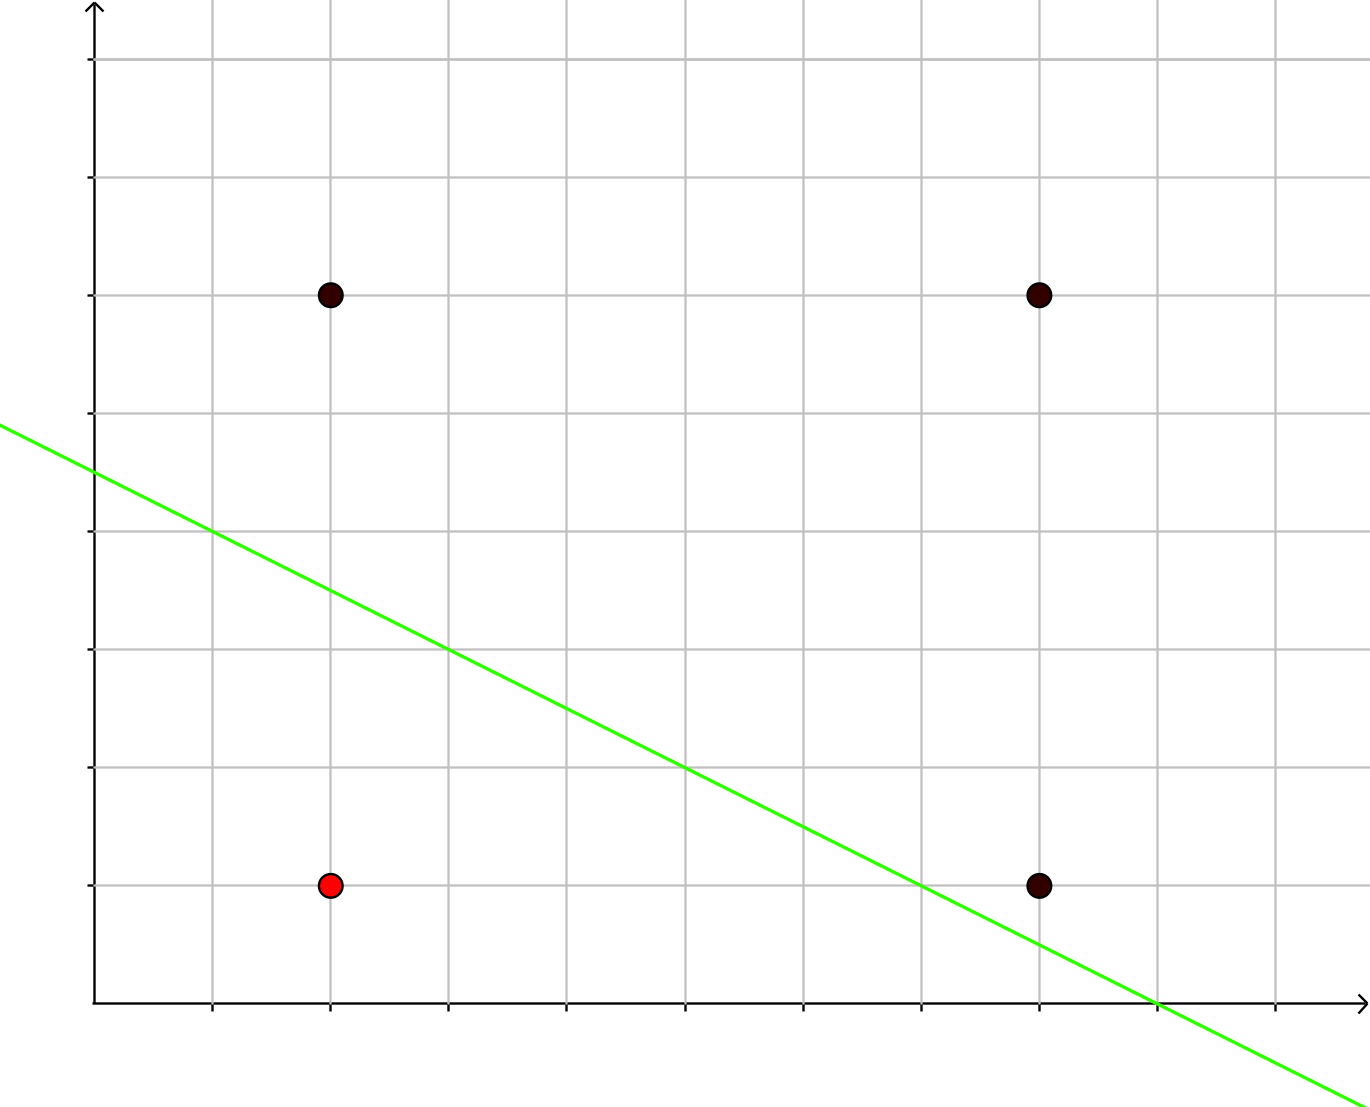
\includegraphics[width=\textwidth]{or}
  \caption{La función lógica \texttt{OR}, en su versión bidimensional, tiene cuatro posibles salidas:
    tres de ellas arrojan un valor positivo, mientras que la otra es negativa. Claramente, se trata de una función
    separable mediante una recta.
    (Elaboración propia.)}
  \label{or-fig}
\end{figure}

Para finalizar esta sección, cabe destacar que la función de activación ($signo$) que acaba de ser presentada\
no es la única (Figura \ref{activations}). En realidad, se buscan opciones más suavizadas y, sobre todo, diferenciables con el fin de\
optimizar los parámetros de modelos más complejos.

\begin{figure}[H]
  \centering
  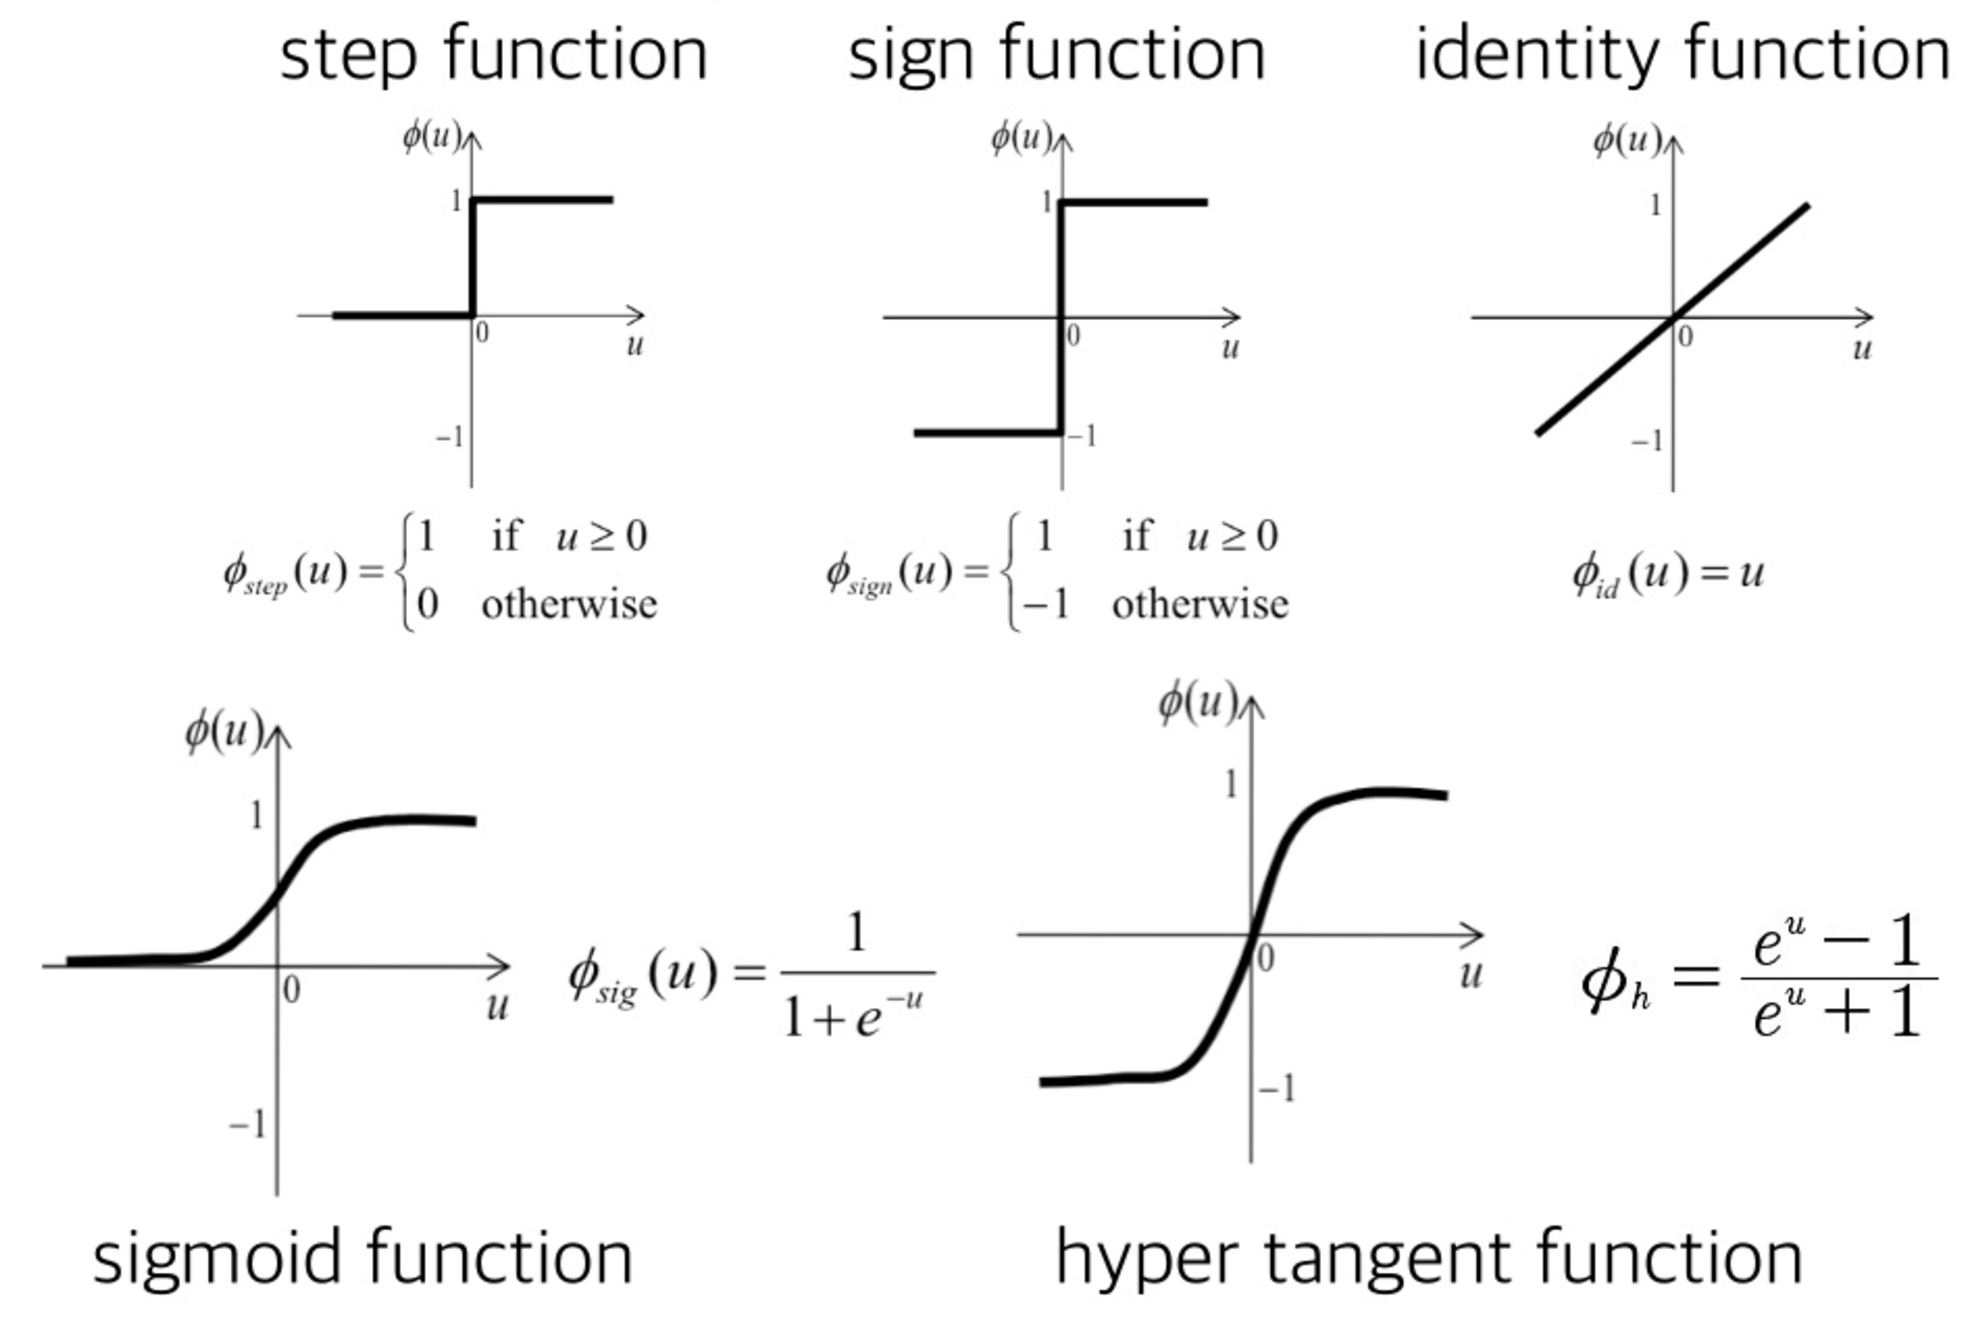
\includegraphics[width=\textwidth]{activations}
  \caption{Las funciones de activación más comunes.
    (Tomado de (\url{https://www.slideshare.net/SungJuKim2/multi-layer-perceptron-back-propagation}))}
  \label{activations}
\end{figure}

\subsection{El perceptrón multicapa}

\noindent
El contenido de este apartado se basa principalmente de \cite{haykin2009} y \cite{rojas1996}.\par
No todos los patrones de datos son linealmente separables. Por ejemplo, la función lógica \verb+XOR+, contiene\
salidas cuyos valores no pueden ser divididos en dos partes del plano sin ser mezclados. Por consiguiente,\
es necesario aumentar la capacidad de cómputo del perceptrón. Combinaremos, ahora, varios perceptrones\
en una \emph{red neuronal de propagación hacia adelante}, estructurando el cómputo en distintas\
\emph{capas ocultas}.\par
El flujo de la información irá de capa en capa, en una sola dirección hasta llegar a una \emph{capa de salida}.
Cada capa oculta consta de un conjunto de neuronas, sin conexiones entre ellas, pero totalmente conectadas a la\
capa inmendiatamente anterior y posterior. A este modelo se le conoce comúnmente como\
\textbf{perceptrón multicapa} (\emph{MLP} por sus siglas en inglés) y es el punto de partida de la rama\
del aprendizaje automático conocida como \textbf{aprendizaje profundo} (\emph{deep learning} por sus siglas en inglés).

\begin{figure}[H]
  \centering
  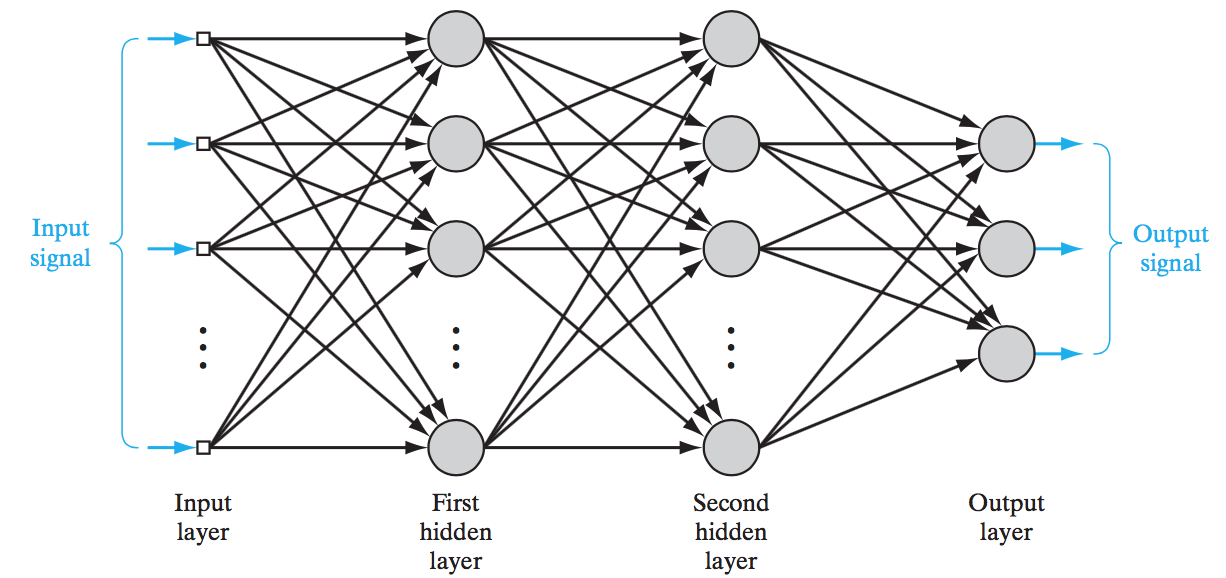
\includegraphics[width=\textwidth]{mlp}
  \caption{Arquitectura de un MLP con dos capas ocultas.
    (Tomado de \cite{haykin2009}.)}
\end{figure}

El flujo del cómputo en un MLP puede ser pensado como la composición de las capas ocultas, vistas como funciones que\
procesan los datos de entrada. Formalmente, dado un vector de entrada $\mathbf{x}$, la primera capa oculta $h_1$\
calcula su valor utilizando una matriz de pesos $\mathbf{W_1}$, un sesgo $\mathbf{b_1}$ de la siguiente manera:
\begin{equation}
  h_1 = \sigma\left(\mathbf{W_1}^\top \mathbf{x} + \mathbf{b}_1\right), \label{mlpfirst}
\end{equation}
donde $\sigma$ es una función de activación no lineal y \emph{diferenciable}.\
Las dimensiones de $\mathbf{W}$ corresponden a la entrada y al número de neuronas en la capa $h_1$.\
La $i+1$-ésima capa oculta de un MLP actualiza su valor a partir de la $i$-ésima mediante
\begin{equation}
  h_{i+1} = \sigma\left(\mathbf{W_{i+1}}^\top h_i + \mathbf{b}_{i+1}\right), \label{mlphidden}
\end{equation}
es decir, cada capa tendrá una matriz de pesos y un vector de sesgos propio. La salida, suponiendo que\
hay $m$ capas ocultas, obtiene su valor con la ecuación
\begin{equation}
  \hat{y} = \sigma\left(\mathbf{W_{m+1}}^\top h_m + \mathbf{b}_{m+1}\right). \label{mlpoutput}
\end{equation}
Obsérvese que es posible que $\hat{y}$ tenga más de una dimensión, entonces, cada uno de los valores de dicho\
vector codificará ``la existencia'' de alguna característica en particular. Esto es muy útil para aprender\
clasificadores cuyo codominio es mayor al conjunto binario.\par
En ocasiones, al subgrafo dirigido formado por las capas ocultas $h_i$ y $h_{i+1}$ se le conoce como\
\emph{capa densa} o \emph{totalmente conectada} y es común encontrarla en arquitecturas de mayor complejidad\
y especialización. El MLP está dentro del ``estado del arte'' de los algoritmos de clasificación automática y\
será parte fundamental de los dos modelos neuronales que compone a la arquitectura de procesamiento de imágenes\
y generación de lenguaje de la presente tesis. La parte más importante de ello recae en su algoritmo de\
entrenamiento.\par
A veces conviene generalizar la función de activación de una capa oculta a una función multivariada,\
la cual esté en concordancia con las dimensiones de salida. Por ejemplo, la función $softmax$ generaliza\
la función \emph{sigmoide} expuesta en la Figura \ref{activations}:\
sea $\mathbf{a}_{i+1}^j = (\mathbf{W_{i+1}}^\top h_i)^j + \mathbf{b}_{i+1}^j$ la $j$-ésima neurona\
de la combinación lineal de la $i+1$-ésima capa, entonces
\begin{equation}
  softmax(\mathbf{a})_j = \frac{e^{\mathbf{a}_j}}{\sum_{k=1}^K e^{\mathbf{a}_k}},
\end{equation}
donde asumimos que la salida es un vector de dimensión $K$.

\subsection{Retroalimentación para aprender}

\noindent
El contenido de este apartado se basa principalmente de \cite{goodfellow-et-al-2016}.\par
Como cualquier arquitectura de aprendizaje supervisado, a un MLP debe de asociarse una función objetivo\
(o de \emph{error}) $J$, que le permita estructurar un entrenamiento. La no-linealidad de las funciones de\
activación causan que no se garantice la convexidad por parte de las funciones de error más comunes. Al\
no existir un método analítico para encontrar mínimos sin importar la elección de $J$, el entrenamiento\
de un MLP (y, en general, de una red neuronal profunda) se basa en métodos iterativos que van optimizando\
los parámetros de la arquitectura, tales como optimizadores basados en gradientes.\par
Para estar \textit{ad hoc} a la práctica, presentaremos un algoritmo de \emph{descenso por el gradiente estocástico},
el cual, a pesar de no garantizar la convergencia hacia un punto mínimo, funciona bien sabiendo\
escoger los valores adecuados de inicialización. Dada la salida $\hat{y}$ establecida en la Ecuación\
\ref{mlpoutput}, definimos la función de error total del MLP como
\begin{equation}
  J(\bm{\theta}) = \frac{1}{2n} \sum_{i=1}^n (\hat{y}_i - y_i)^2 \label{mlperror}
\end{equation}
donde $\bm{\theta}$ es el conjunto de los parámetros del MLP, es decir, $\bm{\theta} := \bigcup\{\bm{W}_i, \bm{b}_i\}_{i=1}^n$;\
$n$ es el número de capas del MLP; e $y_i$ es la $i$-ésima etiqueta\
de entrenamiento. A esta función se le conoce como \emph{error cuadrático medio}; en general,
una función de error $J$ se define conceptualmente como la \textbf{entropía cruzada}\
de las distribuciones de los datos ($y \equiv p_{\text{DATOS}}$) y del modelo ($\hat{y} \equiv \hat{p}_{\text{MLP}}$).\
Esto es, la esperanza de la verosimilitud logarítmica negativa del modelo%
\footnote{
  Suponiendo que $p_{\text{DATOS}}$ es una distribución \emph{normal},\
  se puede demostrar la igualdad entre las Ecuaciones \ref{crossentropydef} y \ref{mlperror}.
 }:
\begin{align}
  J(\bm{\theta}) &=  - \mathbb{E}_{p_{\text{DATOS}}} \log\hat{p}_{\text{MLP}}(\bm{x}) \label{crossentropydef}\\
  &= - \sum_i (y_i\log(\hat{y}_i) + (1 - y_i)\log(1 - \hat{y}_i)). \label{crossentropy}
\end{align}
Esta función es particularmente útil si se desea interpretar las salidas del MLP como probabilidades, ya que,\
$\sum_i \hat{y}_i = 1$ y $0 < \hat{y}_i < 1 $ para $1 \leq i \leq n$. Cabe destacar que ambas funciones\
son completamente diferenciables y los procedimientos de optimización, basados en gradientes, son invariantes.

\subsubsection{Propagación hacia atrás}

\noindent
Cualquier algoritmo de optimización basado en gradientes necesita de un método (\emph{eficiente}) para calcular\
las derivadas de los parámetros del modelo. En la literatura de aprendizaje profundo el cálculo de $\hat{y}$\
muchas veces se le conoce como \emph{propagación hacia adelante}. Esto da lugar al algoritmo de\
\textbf{propagación hacia atrás} (o \emph{retropropagación}) que permite que el error resultante $J$ se\
propague de adelante hacia atrás, a través de todos los parámetros del MLP. El objetivo principal de este\
algoritmo será el cómputo del gradiente del modelo $J$ con respecto a los parámetros $\bm{\theta}$, es decir,\
$\nabla_{\bm{\theta}} J(\bm{\theta})$.\par
Para empezar, el algoritmo de propagación hacia atrás se fundamenta en la regla de la cadena del\
\emph{cálculo infinitesimal} para el cómputo de derivadas de composiciones de funciones:\
dados $x \in \mathbb{R}$, $y = g(x)$ y $z = f(g(x)) = f(y)$, la derivada de $z$ con respecto a $x$ se obtiene por
\begin{equation}
  \frac{dz}{dx} =  \frac{dz}{dy} \frac{dy}{dx}.
\end{equation}
Esta noción se generaliza a funciones que involucran la composición de más de dos funciones:\
si
\begin{itemize}
\item $\mathbf{x} \in \mathbb{R}^m$,
\item $\mathbf{y} \in \mathbb{R}^n$,
\item $g: \mathbb{R}^m \to \mathbb{R}^n$,
\item $f: \mathbb{R}^n \to \mathbb{R}$,
\item $\mathbf{y} = g(\mathbf{x})$ y
\item $z = f(\mathbf{y})$, entonces
\end{itemize}
\begin{equation}
  \frac{\partial z}{\partial x_i} =
  \sum_j \frac{\partial z}{\partial y_j} \frac{\partial y_j}{\partial x_i}. \label{multichain}
\end{equation}
En forma vectorial, la Ecuación \ref{multichain} se escribe como
\begin{equation}
  \nabla_{\mathbf{x}} z =
  \left(\frac{\partial y}{\partial x}\right)^\top \nabla_{\mathbf{y}} z. \label{vectchain}
\end{equation}\par
De la Ecuación \ref{vectchain} vemos que la expresión $\frac{\partial \mathbf{y}}{\partial \mathbf{x}}$\
es la matriz \emph{jacobiana} (de $n \times m$) de $g$, es decir, el gradiente de una variable vectorial\
$\mathbf{x}$ se obtiene multiplicando dicho jacobiano por el gradiente $\nabla_{\mathbf{y}} z$.\
Para cada operación en el \emph{grafo dirigido}, definido en un MLP, el algoritmo de propagación hacia atrás realizará\
un producto entre jacobianos y gradientes.\par
Las derivaciones que restan al presente apartado, fueron basadas de \cite{website:umontreal:deeplearning}.\par
En la práctica, el cómputo de estos gradientes es invariante si en vez de vectores tenemos tensores.\
Intuitivamente, uno puede pensar que, previamente a correr propagación hacia atrás, cualquier tensor\
de dimensiones $n \times m \times p$ se \emph{aplane} a un vector de dimensión $1 \times nmp$. Tras el\
cálculo de los gradientes, los vectores aplanados vuelven a su representación \emph{tensorial}.\par
Mediante la regla de la cadena, es posible desarrollar una expresión para el cálculo del gradiente\
de $J$ con respecto a todos los parámetros $\bm{\theta}$ del MLP. Sin embargo, una implementación\
\emph{ingenua} involucraría que el cálculo de muchas subexpresiones se repita un número considerable de veces.\
En muchas ocasiones, calcular la misma expresión más de una vez resulta una pérdida de tiempo y/o memoria,\
la cual muchas veces puede significar un gasto de orden exponencial con respecto al número de parámetros.\par
En términos formales, consideremos a $u$ como una neurona de la capa $k+1$ de un MLP arbitrario y que recibe como entradas\
las salidas de las neuronas $v_1, v_2, \ldots, v_m$ de la capa $k$. De acuerdo a la Ecuación \ref{vectchain},\
el gradiente de la función de error $J$ con respecto a $u$ se obtiene mediante
\begin{equation}
  \nabla_{u} J =
  \left(\frac{\partial \bm{v}}{\partial u}\right)^\top \nabla_{\bm{v}} J, \label{neurongradient}
\end{equation}
donde $\bm{v} = (v_1, v_2, \ldots, v_m)$. Este es un proceso recursivo que inicia con el cómputo del gradiente\
para la última capa, en donde $\frac{\partial J}{\partial J_i} = 1$ para toda neurona de salida $J_i$.\
Nótese que si para obtener $J$ se requirieron $n$ nodos y cada uno de éstos requiere un tiempo constante de\
cómputo más $m$ arcos, entonces calcular $\nabla_{u} J$ requiere al menos $\Omega(m)$ cómputos y no es posible\
obtener los gradientes de una manera más rápida.\par
Remembrando la terminología establecida a partir de las Ecuaciones \ref{mlpfirst} y \ref{mlphidden}, sea
\begin{equation}
  a_k = \bm{b}_k + \bm{W}_kh_{k-1} \label{mlplinearcomb}
\end{equation}
la ecuación que define la combinación lineal que determina las salidas de la $k$-ésima capa de un MLP.\
En lo secuente, utilizaremos a la función de error por entropía cruzada (Ecuación \ref{crossentropydef}) y asumimos,\
sin pérdida de generalidad, como funciones de activación $\sigma = softmax$ para la última capa\
y $\sigma = \tanh$ para las capas ocultas. Asumiendo que hay $L$ capas en un MLP,\
es importante enfatizar en las siguientes observaciones:
\begin{align}
  \frac{\partial(-\log \hat{y})}{\partial a_{L, i}} &= \hat{y}_i - \mathbbm{1}_{y=i}, \label{derivlosscomb}\\
  \frac{\partial \tanh(u)}{\partial u} &= 1 - \tanh(u)^2. \label{derivtanh}
\end{align}
Resulta lógico entender que la Ecuación \ref{derivlosscomb} calcula la diferencia que existe entre las salidas\
del MLP y las etiquetas del conjunto de datos. Por otro lado, la Ecuación \ref{derivtanh} calcula las\
derivadas parciales de la función tangente hiperbólica aplicada a cualquier tensor real $u$. Obsérvese\
que de la expresión $a_{L, i}$ nos referimos a la última capa de un MLP mediante su índice, notación\
que hará más fácil escribir el siguiente procedimiento.\par
\begin{itemize}
\item Para la función de error, $\frac{\partial J}{\partial J} = 1$.
\item El gradiente del error con respecto a cada entrada de la última capa:
  \begin{equation}
    \frac{\partial J}{\partial a_{L, i}} =
    \frac{\partial J}{\partial J} \frac{\partial J}{\partial a_{L, i}} =
    \hat{y}_i - \mathbbm{1}_{y=i}. \label{derivtanh}
  \end{equation}
\item Para cada capa, desde $k = L$ bajando hasta 1:
  \begin{itemize}
  \item calculamos el gradiente con respecto a los sesgos:
    \begin{equation}
      \frac{\partial J}{\partial \bm{b}_{k, i}} =
      \frac{\partial J}{\partial a_{k, i}} \frac{\partial a_{k, i}}{\partial \bm{b}_{k, i}} =
      \frac{\partial J}{\partial a_{k, i}}, \label{biasgradient}
    \end{equation}
  \item calculamos el gradiente con respecto a los pesos:
    \begin{equation}
      \frac{\partial J}{\partial \bm{W}_{k, i, j}} =
      \frac{\partial J}{\partial a_{k, i}} \frac{\partial a_{k, i}}{\partial \bm{W}_{k, i, j}} =
      \frac{\partial J}{\partial a_{k, i}} h_{k-1, j}, \label{biasgradient}
    \end{equation}
  \item propagamos el gradiente hacia una capa inferior; para $k > 1$:
    \begin{align}
      \frac{\partial J}{\partial h_{k-1, j}} &=
      \sum_i \frac{\partial J}{\partial a_{k, i}} \frac{\partial a_{k,i}}{\partial h_{k-1, j}} =
      \sum_i \frac{\partial J}{\partial a_{k,i}} \bm{W}_{k, i, j}, \label{hiddenbackprop}\\
      \frac{\partial J}{\partial a_{k-1, j}} &=
      \frac{\partial J}{\partial h_{k-1, j}} \frac{\partial h_{k-1, j}}{\partial a_{k-1, j}} =
      \frac{\partial J}{\partial h_{k-1, j}} (1 - h_{k-1, j}^2). \label{combbackprop}
    \end{align}
  \end{itemize}
\end{itemize}

\subsubsection{Descenso por el gradiente}

\noindent
Una vez obtenido el diferencial por el cual se va a optimizar un MLP con respecto a la función\
de error, lo que procede es actualizar los parámetros de la red neuronal con una cantidad adecuada.\
\emph{Descenso por el gradiente} es un algoritmo que minimiza la función de error $J(\bm{\theta})$\
de una red neuronal (en general) mediante la actualización de los parámetros $\bm{\theta} \in \mathbb{R}^d$\
en dirección opuesta al gradiente $\nabla_{\bm{\theta}}J(\bm{\theta})$.\par
En su versión más sencilla, este algoritmo intenta encontrar un mínimo (local) mediante un proceso\
iterativo en el que el gradiente $\nabla_{\bm{\theta}}J(\bm{\theta})$ se calcula y se actualizan \emph{todos}\
los parámetros en proporción con el \emph{meta}-parámetro $\eta$, conocido como \textbf{tasa de aprendizaje}.\
El número $\eta$ determina el \textit{tamaño de los pasos} que se deben tomar para llegar al\
mínimo local. Así,
\begin{equation}
  \bm{\theta} = \bm{\theta} - \eta \nabla_{\bm{\theta}}J(\bm{\theta}). \label{vanillagd}
\end{equation}\par
La Ecuación \ref{vanillagd} implica que hay que calcular los gradientes por cada parámetro del\
conjunto de datos para realizar \emph{una sola} actualización. Esto deriva en un procedimiento\
realmente lento e incluso intratable para conjuntos de datos que no quepan en memoria. La lentitud\
se justifica por el cómputo redundante de varios gradientes para entradas similares antes\
de actualizar cada parámetro. Para sobreponerse a este problema, se da lugar al algoritmo de\
\emph{descenso por el gradiente estocástico} (\emph{SGD}, por sus siglas en inglés)\
en el cual se realiza una actualización por cada ejemplar $(x^{(i)}, y^{(i)})$ del conjunto de datos:
\begin{equation}
  \bm{\theta} = \bm{\theta} - \eta \nabla_{\bm{\theta}}J(\bm{\theta}; x^{(i)}; y^{(i)}). \label{sgd}
\end{equation}
Potencialmente, SGD permite llegar a mejores mínimos locales a los que converge la primera\
versión descrita. Por otro lado, es más probable que no se pueda llegar al mínimo global, dada\
la fluctuación que puede haber en las primeras actualizaciones. Sin embargo, se puede demostrar\
que si la tasa de aprendizaje es suficientemente pequeña, es casi segura la convergencia hacia\
un mínimo local.\par
En la práctica, la versión implementada en la mayoría de las bibliotecas de aprendizaje automático\
incorpora lo mejor de las Ecuaciones \ref{vanillagd} y \ref{sgd}:
\begin{equation}
  \bm{\theta} = \bm{\theta} - \eta \nabla_{\bm{\theta}}J(\bm{\theta}; x^{[i:i+n]}; y^{[i:i+n]}). \label{minibatchgd}
\end{equation}
Cada actualización propuesta por la Ecuación \ref{minibatchgd} se da en un rango de los datos,\
conocido como \textbf{mini-lote} o, simplemente, \emph{lote}. Esto permite que la covergencia se de\
de manera más estable. Además, el tamaño del lote $n$ usualmente varía entre 50 y 256. El número\
de veces que el algoritmo ve el conjunto de datos entero se le llama número de \textbf{épocas}\
Por otro lado, definimos al número de \emph{iteraciones} del algoritmo,\
contando el número de veces que cada lote pasa por el mismo. El Procedimiento \ref{minibatchgdcode}\
describe una implementación del algoritmo de descenso por el gradiente utilizado en muchas bibliotecas\
actuales de aprendizaje automático.
\begin{lstlisting}[language=Python,
    caption={
      Implementación del algoritmo de descenso por el gradiente utilizando mini-lotes, en lenguaje
      Python. Antes de iterar sobre todos los lotes, se mezclan los datos de manera aleatoria.
    },
   label=minibatchgdcode
  ]
  for i in range(num_epocas):
  np.random.shuffle(datos)
  for lote in get_lotes(datos, tamanyo_lote=50):
    params_grad = evaluar_gradiente(funcion_error, lote, params)
    params = params - tasa_aprendizaje * params_grad
\end{lstlisting}\par
Visualmente el algoritmo de descenso por el gradiente se puede entender mediante la Figura \ref{visualgd}.\
El componente restante, y que es motivo de investigación, es la manera en la que la tasa de aprendizaje\
se calcula. Para ello, se proponen varios \emph{optimizadores} descritos en \cite{DBLP:journals/corr/Ruder16};\
la elección de su uso depende fuertemente del diseño de la arquitectura en cuestión.

\begin{figure}[H]
  \centering
  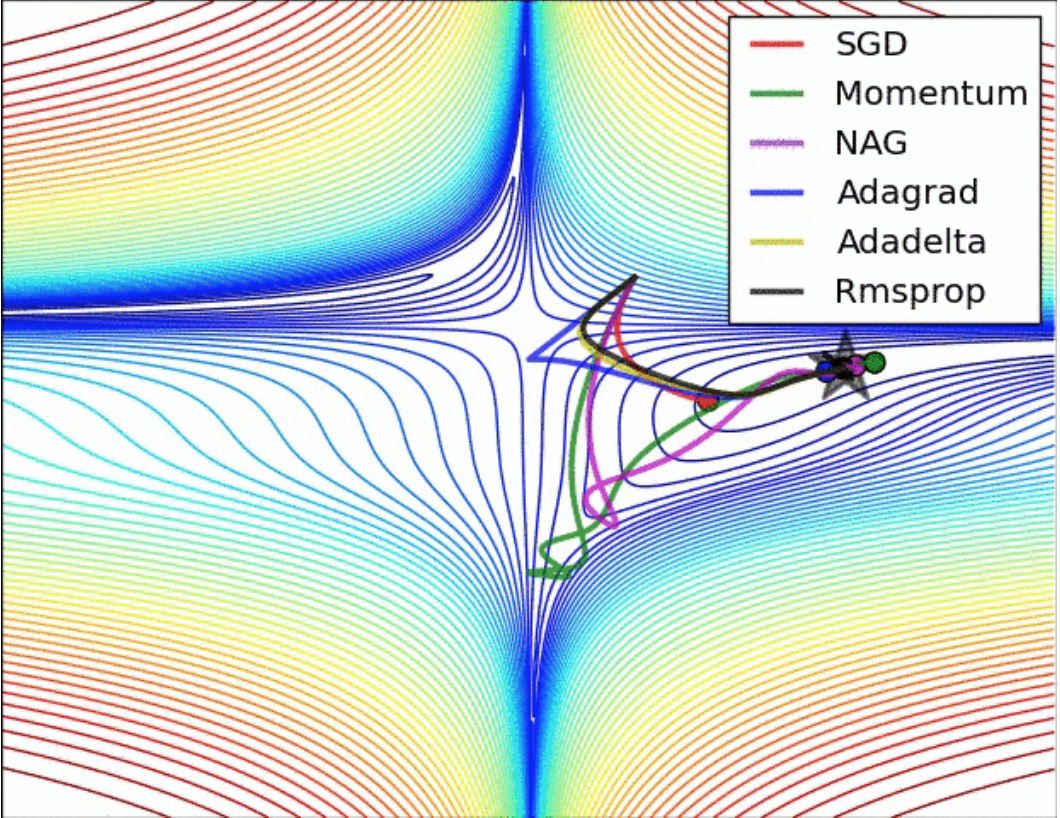
\includegraphics[width=0.5\textwidth]{visualgd}
  \caption{
    La optimización realizada por el algoritmo SGD con mini-lotes. Se muestra
    el comportamiento de distintos optimizadores.
    (Tomado de \cite{DBLP:journals/corr/Ruder16}.)
  }
  \label{visualgd}
\end{figure}

\section{Redes neuronales convolucionales}

\noindent
En 1989, el francés Yann LeCun comenzó a trabajar en los fundamentos de un novedoso modelo\
neuronal basado en la biología de la corteza visual del cerebro animal. Su trabajo, eventualmente,\
lo llevó a ser nombrado director de la investigación en IA en Facebook. Su ascenso\
al \emph{``podio''} del aprendizaje profundo es producto de una revolución en la\
\emph{vanguardia} del reconocimiento de imágenes a través de computadoras. Y lo más probable\
es que el mismo modelo continúe sobresaliendo por algunos años.\par
Como la mayoría de las arquitecturas neuronales, las \textbf{redes neuronales convolucionales}\
(\emph{CNN's}, por sus siglas en inglés) no alcanzaron la popularidad suficiente hasta entrada\
la época reciente, caracterizada por una alta conectividad (a través de Internet) y un incremento\
significativo en la capacidad de cómputo de los dispositivos modernos. Sin embargo, LeCun ya había\
obtenido resultados sobresalientes hacía 1998, en tareas de reconocimiento de patrones \cite{bengio2009}.\
El enfoque de LeCun, y de su equipo en \emph{Bell Labs}, consistió en dar un modelo de mayor\
capacidad en \emph{representaciones internas} que el tradicional perceptrón multicapa.\par
Un aspecto importante en esta arquitectura consiste en la delegación de ciertas partes de la misma\
a sub-problemas específicos de la tarea a resolver. Por consiguiente, cada capa de una CNN definirá\
uno (o varios) niveles de representación, los cuales capturan ciertas características inherentes\
al flujo de datos de entrada. Mediante un basto conjunto etiquetado de datos, se pueden aprender dichas\
abstracciones de manera supervisada.

\subsection{La capa convolucional}

Para iniciar la discusión sobre la estructura de una CNN, usaremos como ejemplo al reconocimiento\
computacional de imágenes; sin embargo, cabe notar que esta arquitectura es popular en tareas donde\
exista la necesidad de reconocer patrones sobre conjuntos de datos con topología \emph{cuadriculada}.\
\footnote{De acuerdo a \cite{goodfellow-et-al-2016}, como ejemplos de datos con una topología cuadriculada,\
  se incluyen series de tiempo (cuadrícula de una dimensión), audio o videos.}
Uno de los conjuntos de datos más famosos, y de mayor tradición, es la \emph{Mixed National Institute of Standards}\
\emph{and Technology database}, mejor conocida como MNIST. En ella se alberga una gran cantidad de dígitos\
escritos a mano; el problema, entonces, consiste en clasificar cualquier manuscrito dado en una de las $10$ clases\
existentes, de acuerdo al dígito más parecido.\par

\begin{figure}
  \centering
  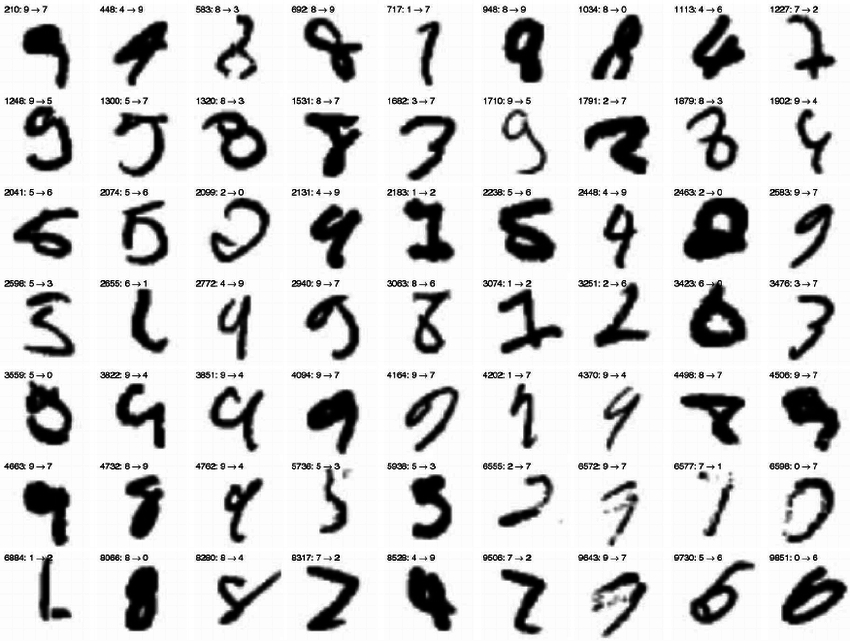
\includegraphics[width=0.6\textwidth]{mnist}
  \caption{Algunos dígitos existentes en la base de datos MNIST.
    (Tomado de \url{http://www.researchgate.net/}.)}
  \label{mnist_fig}
\end{figure}

Como se observa en la Figura \ref{mnist_fig}, existen distintas maneras de escribir a mano un solo dígito. Quisiéramos\
que nuestra solución sea lo suficientemente robusta para distinguir $4$'s de $9$'s por más ilegible que\
sea la letra. No tenemos idea de dónde buscar ciertas características o si el observar un cambio drástico\
en el color de varios pixeles contiguos nos sea significativo; todo esto es parte de lo que se deberá\
\emph{aprender}. Esta incertidumbre en la detección de atributos conduce a, de alguna manera, ir en\
búsqueda de pequeñas porciones de la imagen que nos den una pista por dónde empezar.\par
En este punto cabe recordar que usualmente para una computadora, una imagen es un arreglo de tres dimensiones,\
cada una especificando la posición de un pixel y su color. En la práctica (y de acuerdo a las últimas tendencias\
de programación de redes neuronales), a esta estructura se le llama \textbf{tensor}, por lo que seguiremos\
la convención. Volviendo a nuestra búsqueda, necesitamos un parámetro que nos indique el mínimo de pixeles a\
analizar para empezar a encontrar detalles claves de la imagen. Por ello, vamos a usar un pequeño tensor ``cuadrado''\
para recorrer toda la imagen. A dicho tensor le llamaremos \textbf{filtro} (\emph{kernel}, en inglés).\
Llamaremos \textbf{zancada} (\emph{stride}, en inglés) al número de pixeles que ``saltamos'' (en cualquier dimensión)\
al mover un filtro sobre la imagen. La salida se calcula realizando una combinación lineal sobre cierta región de la\
imagen ponderada con los valores del filtro y añadiendo un sesgo. Esto produce un tensor con una profundidad\
equivalente al número de filtros usados. En símbolos, esto corresponde a realizar lo siguiente
\begin{equation} \label{entry-wise-sum}
  \sum _{i} x_i w_i\ + b
\end{equation}
donde $x_i$ y $w_i$ corresponden a la $i$-ésima entrada de la imagen y del filtro, respectivamente, y $b$ es el sesgo.\par
En ocasiones es conveniente rodear una imagen con ceros, ya que debemos garantizar que el filtro encaje\
exactamente dentro de la imagen conforme se va deslizando horizontal y verticalmente. A esto se le conoce como\
\textbf{relleno de ceros} (\emph{zero-padding} en inglés). Los parámetros que acaban de ser presentados\
constituyen a una \textbf{capa convolucional}, en la cual reside la mayor carga computacional de la arquitectura.\
Para abreviar, en adelante nos referiremos a dicha capa con la sigla \textbf{CONV}.\par
La correcta elección de parámetros debe de garantizar que el filtro no salga de las dimensiones de la imagen\
de entrada (sujeta a relleno de ceros). Supongamos que tenemos una imagen cuadrada de dimensión $W \times W$,\
un filtro de dimensión $F \times F$. Además ``enmarcamos'' (rellenamos) de ceros la imagen con un grosor de $P$\
pixeles y aplicamos el filtro con una zancada $Z$. Entonces, la cantidad de neuronas resultantes (en una dimensión)\
está dada por
\begin{equation}
  \frac{W - F + 2P}{Z} + 1,
\end{equation}
donde este número es un entero positivo.

\begin{figure}
  \centering
  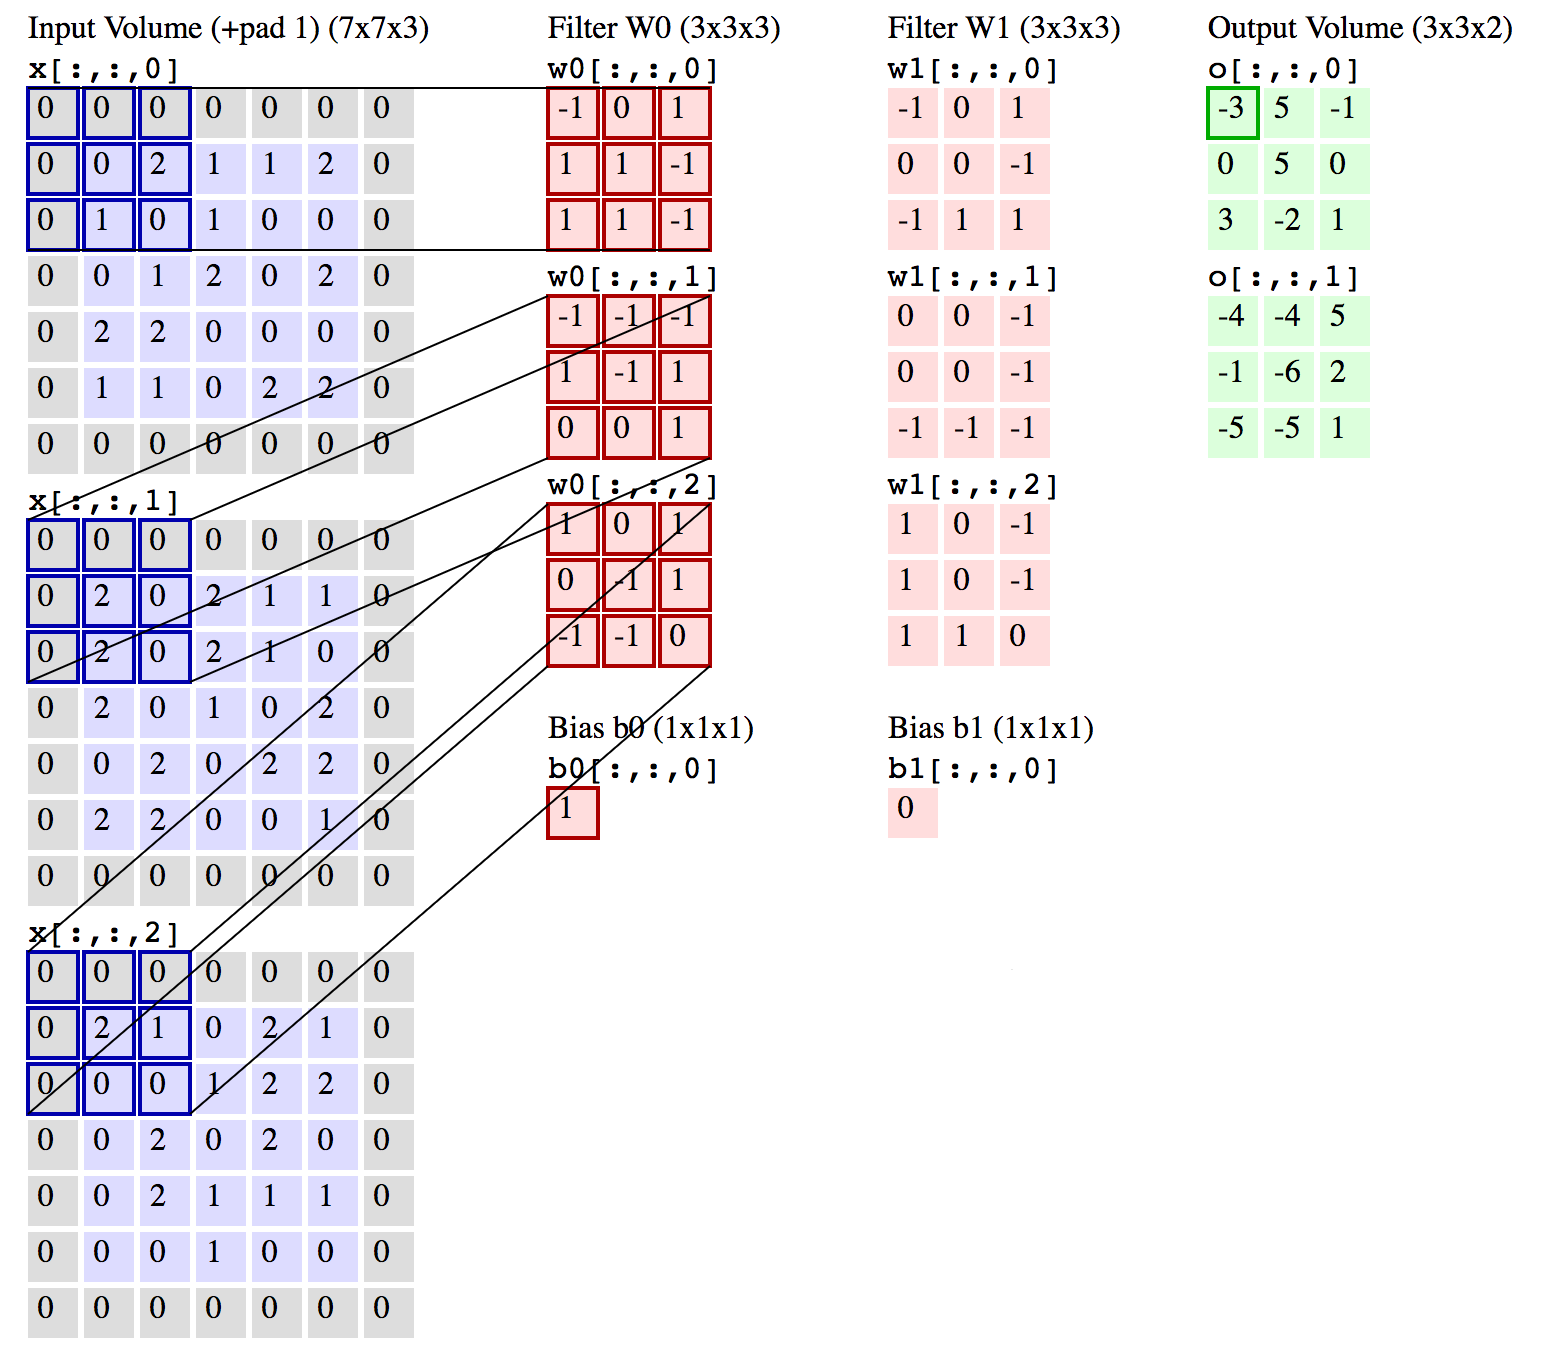
\includegraphics[width=\textwidth]{conv_process}
  \caption{Ilustración de una pequeña capa convolucional.
    Cada imagen de entrada contiene tres niveles de profundidad, con los cuales trabaja
    el filtro (un tensor de pesos). Cabe destacar que cada valor de $x$ está rellenado por ceros.
    Dado que la profundiad del volumen de la salida es sólo 2, hay igual número de filtros en total.
    (Tomado de \url{http://cs231n.github.io/convolutional-networks/}.)}
  \label{fCNN_fig}
\end{figure}

\subsection{La \emph{convolución}}

\noindent
Matemáticamente, este proceso se puede formalizar mediante la convolución de dos funciones reales.\
Si $x$ denota a nuestro dígito desconocido y $w$ a nuestro filtro, entonces la convolución de $x$ con\
$w$, en un punto $t$, se define como:
\begin{equation}
  c(t) := \int x(a) w(t-a) da
\end{equation}
y se denota:
\begin{equation}
  c(t) = (x * w)(t).
\end{equation}
En el mundo digital, tenemos conjuntos de datos discretos, por lo que es conveniente dar una definición\
adaptada al respecto:
\begin{equation}
  c(t) = (x * w)(t) := \sum _{a=-\infty} ^{\infty} x(a) w(t-a).
\end{equation}
Dentro del contexto de reconocimiento de imágenes, es útil especificar que la convolución se hace en dos\
dimensiones de las que se están contemplando. Para ello introducimos la siguiente notación:\
si $i$ y $j$ son valores que denotan la posición de un pixel, $X(i,j)$ es el valor (color) correspondiente\
y $K(i,j)$ denota la entrada $(i,j)$ de nuestro filtro, definimos a la convolución $C$ como:
\begin{equation}
  C(t) = (K * I)(i,j) := \sum_m \sum_n I(i-m,j-n) K(m,n).
\end{equation}
Muchas bibliotecas de redes neuronales utilizan la \textbf{correlación cruzada} en vez de la convolución.\
Semánticamente, la correlación cruzada sirve para analizar lo mismo que buscamos con la convolución; por\
ello, esta sutil distinción muchas veces no es notada. La definición es la siguiente:
\begin{equation} \label{cross_corr}
  C(t) = (I * K)(t) := \sum_m \sum_n I(i+m,j+n) K(m,n).
\end{equation}
Nótese que en las dos últimas definiciones se ha convenido \emph{voltear} los índices del filtro. En la\
teoría, la ventaja que trae esto consiste en una mayor facilidad de probar ciertos resultados.\par
Para terminar de describir la \textbf{capa convolucional} de la arquitectura,\
vale la pena hablar un poco sobre la salida de (\ref{cross_corr}). Aquí estamos\
caracterizando al valor de cada neurona como se describió en (\ref{entry-wise-sum}).\
Al conjunto de tensores resultantes se les conoce, convenientemente, como \textbf{mapas de activación}.\par
Cabe señalar que la eficiencia de la convolución es mucho mayor a la de una\
multiplicación de matrices (en una capa densa) y esto ocurre, principalmente, por las siguientes razones:
\begin{itemize}
\item En una capa densa, se consideran interacciones entre cada neurona de entrada con cada neurona de salida.\
  Es decir, los productos matriciales involucran a cada pixel, sin importar qué lugares en específico son\
  los que vale la pena resaltar.
\item Se dice que en una capa convolucional se manejan \textbf{pesos dispersos}, los cuales corresponden\
  a las entradas del filtro. Esto significa que después de un entrenamiento, el filtro aprenderá a interactuar\
  con ciertos grupos de pixeles, sin conocer su distribución. Con esto es posible tomar en cuenta pequeños\
  detalles que ocurren en una vecindad reducida de pixeles.
\item En una capa convolucional, los pesos del filtro que se buscan aprender son mucho menos que los pesos que\
  se aprendería en una capa densa: si la imagen de entrada contiene miles o millones de pixeles, entonces\
  necesitamos cientos de pixeles en nuestro filtro para aprender los razgos más pequeños de la misma (como\
  bordes o puntos).
\end{itemize}\par
En resumen, si tenemos $m$ entradas y $n$ salidas en una capa, y ésta es densa, entonces habremos de realizar\
$O(m \times n)$ operaciones para calcular la salida. En cambio, en una capa convolucional, podemos tener\
una zancada $Z$ de pixeles en el filtro, con un orden de magnitud mucho menor a $n$; lo cual va a provocar\
que sea más eficiente calcular $O(m \times Z)$ operaciones.

\subsection{Filtros vistos como arreglos de neuronas}

\noindent
Dependiendo del número de filtros escogidos para aplicarse en la capa CONV, se definirá la salida de la misma.\
Intuitivamente, si se usan $12$ filtros en una imagen cuya dimensión de entrada es de $32 \times 32 \times 3$,\
uno puede imaginarse $12$ imágenes procesadas por la capa CONV, como resultado del procesamiento REF-IMAGEN.\
Es decir, la dimensión de la salida sería de $32 \times 32 \times 12$.\par
Esto no corresponde al ``mecanismo canónico'' que caracteriza a una capa neuronal (densa), en donde todas las entradas\
participan en la decisión de la salida. Más aún, a diferencia del perceptrón multicapa, en donde existe un conjunto\
de pesos para cada neurona, aquí un conjunto de neuronas comparte los mismos pesos.\
Sin embargo, podemos ahorrarnos la discusión sobre cómo adaptar al algoritmo de propagación hacia atrás para\
hacer que cada neurona aprenda, transformando un poco la arquitectura:
\begin{itemize}
\item Si nuestra dimensión de entrada es de $32 \times 32 \times 3$, ``aplanamos'' dicho tensor de manera vertical,\
  es decir, en uno de dimensión $1024 \times 1 \times 3$.
\item Por cada filtro, apilamos todas las neuronas en una salida cuya altura está determinada por el valor de la zancada.
\item Cada neurona de salida estará conectada a tantas neuronas de entrada como indique, otra vez, la zancada. Éstas\
  serán contiguas tras ser transformadas como indica el primer punto mencionado. Adicionalmente, podemos pensar\
  que todas las demás neuronas de entrada están conectadas a cada salida con un peso equivalente a cero unidades.
\item En este caso, los valores que constituyen al tensor de filtro estarán codificados como pesos en cada sinapsis.
\item La $i+1$-ésima neurona de salida tendrá como primera entrada (en orden de arriba hacia abajo), a la segunda\
  entrada de la $i$-ésima neurona.
\end{itemize}\par
La capa de salida de este reacomodo corresponde a un mapa de activación ``aplanado''. Si queremos un \emph{volumen}\
de salida con 12 mapas, entonces habrá que visualizar un modelo en el cual tenemos 12 mapas aplanados conectados, cada uno,\
al tensor de entrada y sin sinapsis alguna entre cada uno de éstos. Cabe destacar que durante el entrenamiento,\
basta actualizar únicamente un solo conjunto de pesos que conectan a una neurona de salida con una cantidad de entradas\
equivalente al valor de la zancada y, posteriormente, propagar los nuevos valores a los demás pesos por cada neurona de\
salida; esto por cada uno de los filtros. Esto ocurre debido a que cada uno de los filtros \emph{``comparte parámetros''},\
como se observa en la figura \label{fCNN_fig}.

\begin{figure}
  \centering
  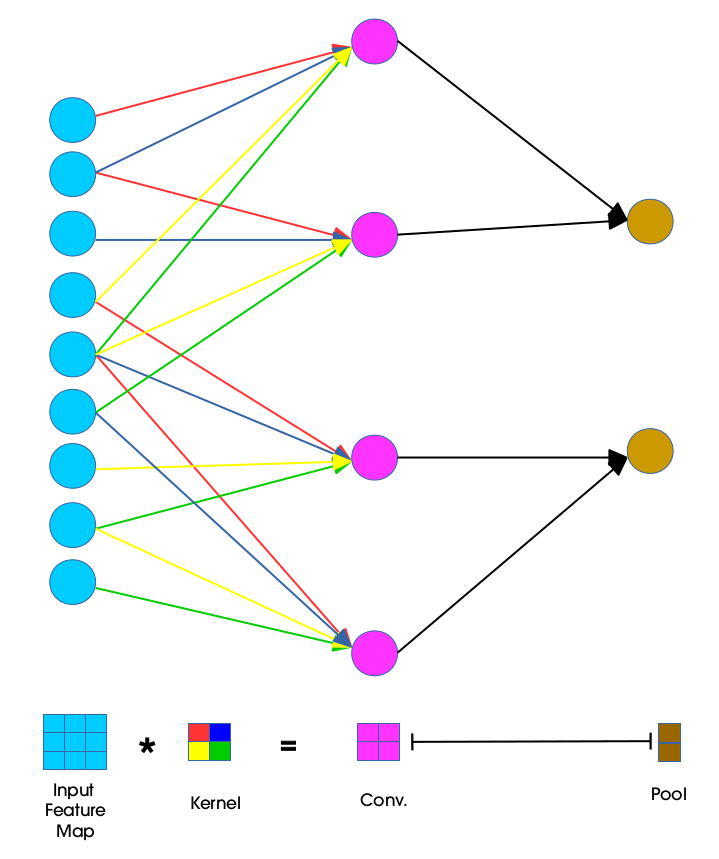
\includegraphics[width=0.65\textwidth]{fCNN}
  \caption{El concepto de pesos compartidos. Las sinapsis del mismo color representan conexiones con pesos iguales.
    En este caso, se tendría una zancada de 4 neuronas.
    (Tomado de \url{http://www.jefkine.com/general/2016/09/05/backpropagation-in-convolutional-neural-networks/}.)}
  \label{fCNN_fig}
\end{figure}

\subsection{La \emph{``capa''} de activación}

\noindent
Como sucede al calcular las salidas de una capa densa, aquí hay que utilizar una función no lineal (y \emph{suave}) para\
finalizar la clasificación. En algunos casos, a este paso se le suele llamar \textbf{capa de no linealidad}.\
En \cite{lecun2010}, además de usar dicho término, se propone a la función $tanh$, sobre cada entrada de los\
mapas de activación, como el estándar en CNN's. Sin embargo, también se señala que una \emph{sigmoide}\
\emph{rectificada} ha dado buenos resultados en reconocimiento de imágenes (sujeta a una normalización posterior);\
el caso particular es el de la \textbf{unidad lineal rectificada} (\emph{ReLU}, por sus siglas en inglés):
\begin{equation}
  f(x) = \max(0, x).
\end{equation}

\begin{figure}
  \centering
  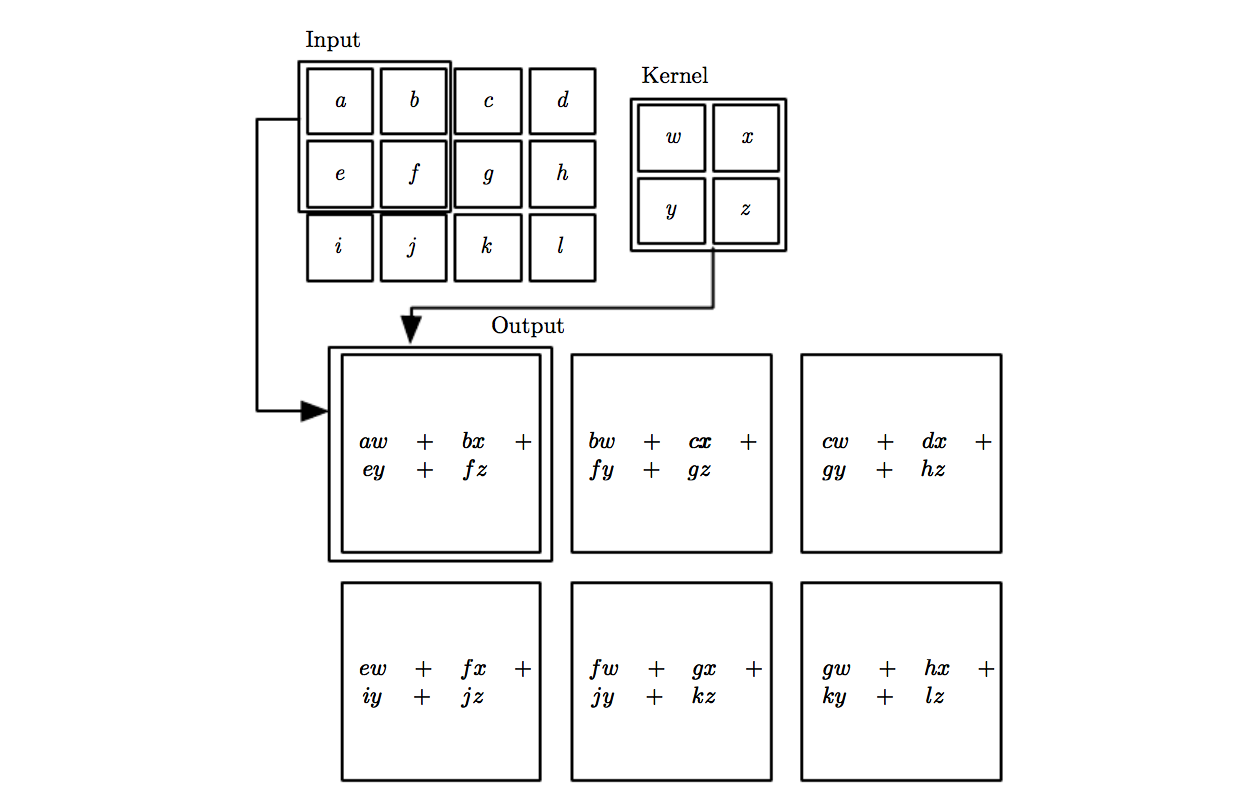
\includegraphics[width=0.9\textwidth]{2dconv}
  \caption{Ilustración del proceso de convolución. El filtro se desliza por la imagen de entrada y
    se efectúa un producto pixel por pixel.)
    (Tomado de \cite{goodfellow-et-al-2016}.)}
  \label{2dconv_fig}
\end{figure}

\subsection{La capa de \emph{pooling}}

\noindent
Un exceso de aprendizaje en la capa de convolución puede provocar un \emph{sobreajuste} sobre\
el modelo. Esto se puede observar, en nuestro ejemplo, con una arquitectura donde cada filtro\
se entrene a funcionar para un grupo pequeño y exclusivo de pixeles, los cuales esperen encontrar\
detalles claves en lugares precisos. Es necesario, entonces, ocuparse de que una CNN\
\emph{generalice} suficientemente su aprendizaje para aumentar su robustez.\par
Por ello, las CNN's llevan, además de capas convolucionales, algunas capas de \textbf{agrupación}\
(\emph{pooling}, en inglés y usaremos esta palabra en adelante) con las cuales se puede extraer\
los detalles más fundamentales de cada mapa de activación. En la práctica, existen dos operaciones\
de \emph{pooling} que sobresalen sobre las demás: \emph{max}-\emph{pooling} y \emph{avg}-\emph{pooling}. Para calcular cualquier\
capa de \emph{pooling}, se define una vecindad en cada mapa de activación (que no exceda su zancada);\
acto seguido, dependiendo del \emph{pooling} a usar, se almacena el máximo o el promedio de los pixeles\
abarcados en la vecindad.\par
Con esta capa, la arquitectura convolucional se vuelve \textit{aproximadamente \emph{invariante}} a modificaciones\
en la entrada. Esto permite enfocarnos más en la existencia de ciertas características en la imagen\
que en la posición exacta de las mismas.\par
El \emph{pooling}, además, nos brinda un mecanismo de disminución de parámetros del modelo (neuronas)\
brindando la posibilidad de optimizar mucho más la memoria utilizada y las dimensiones de las capas.

\begin{figure}
  \centering
  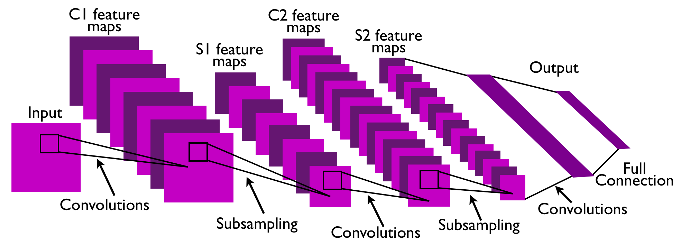
\includegraphics[width=0.8\textwidth]{convnet}
  \caption{Estructura básica de una red neuronal convolucional, con dos fases de extracción de características.
    (Tomado de \cite{lecun2010})}
  \label{convnet_fig}
\end{figure}


\section{Redes neuronales recurrentes}

\noindent
Es frecuente encontrar situaciones en las que exista un orden secuencial entre los datos de entrenamiento.\
Esto es algo que tienen en común tareas como reconocimiento del habla o traducción automática (de idiomas).\
Aquí cada instancia de un conjunto de datos se puede ver como una sucesión de valores
\[\mathbf{X} = \mathbf{x}^{(1)},\ldots,\mathbf{x}^{(\tau)}\]
y el objetivo es entrenar una arquitectura que nos permita predecir $\mathbf{x}^{(i+1)}$,\
dados $\mathbf{x}^{(1)},\ldots,\mathbf{x}^{(i)}$.\par
Un modelo (\emph{estadístico}) de lenguaje es una función de probabilidad sobre cualesquiera sucesiones de símbolos\
de un alfabeto dado. En procesamiento de lenguaje natural (\textbf{PLN}), modelar un lenguaje consiste en\
la construcción de estimadores que tengan la capacidad\
de estructurar oraciones dado un conocimiento \emph{a priori} ($\mathbf{x}^{(1)},\ldots,\mathbf{x}^{(i)}$),\
es decir, maximizar
\begin{equation}
  P(\mathbf{x^{(i+1)}}\ |\ \mathbf{x}^{(1)},\ldots,\mathbf{x}^{(i)}).
\end{equation}
El lenguaje natural es inherentemente ambiguo; hecho que ha popularizado el enfoque probabilístico en PLN, dejando\
atrás arquitecturas puramente simbólicas cuya capacidad de cómputo es limitado. Por ejemplo, el enunciado\
\emph{``Eutropio acomodó el portafolio que Porfirio tiró en el buró''} se puede interpretar de dos maneras:
\begin{itemize}
\item Eutropio encontró el portafolio en el buró y procedió a acomodarlo en algún otro lugar.
\item Porfirio dejó tirado el portafolio; acto seguido, Eutropio lo colocó en el buró.
\end{itemize}\par
En un modelo de lenguaje, ¿cómo decidimos qué interpretación semántica tomar? En la práctica, esto depende del\
contexto (conjunto de datos) y la tarea específicamente a resolver. En términos formales, existe más de un\
\emph{árbol de análisis sintáctico} que caracteriza al enunciado anterior y el modelo debe de encontrar qué árbol tomar\
como interpretación.\par
La teoría de lenguajes formales establece que la elaboración de árboles sintácticos, de gramáticas no ambiguas, es un proceso que requiere\
un modelo computacional que necesariamente utilice al menos una \emph{memoria temporal}. Pero, en general, la ambigüedad\
semántica nos obliga a no poder acotar el tamaño de dicha memoria, por lo que necesitamos una arquitectura \emph{turing-completa}\
al menos para fines de construcción de enunciados sintáctica y semánticamente correctos.\par
Un \textbf{red neuronal recurrente} (\emph{RNN}, por sus siglas en inglés) es una arquitectura que posee una memoria interna.\
La estructura básica de la misma se muestra en la Figura \ref{recurrent_fig}. Podemos observar que la estrategia gráfica para incorporar\
a dicha memoria consiste en establecer un \emph{ciclo} entre la salida y la entrada, es decir, existirá una matriz de pesos que se entrenará y guardará\
un resumen de los aspectos importantes de cada símbolo de la sucesión $\mathbf{X}$ que va procesando.

\begin{figure}
  \centering
  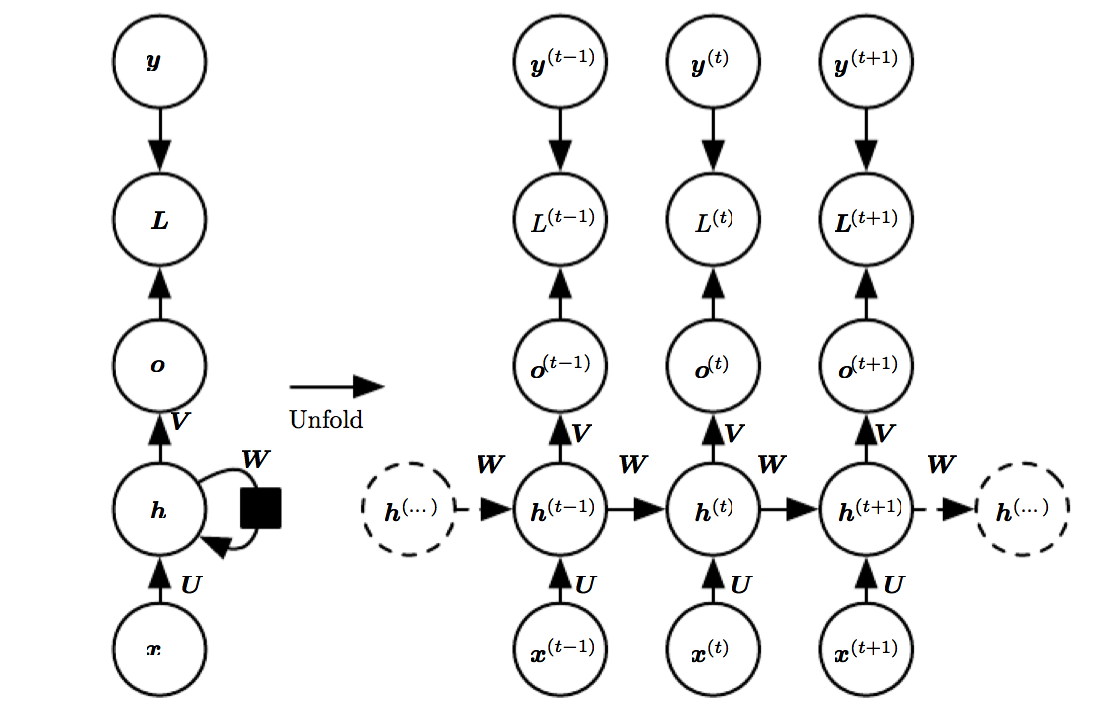
\includegraphics[width=\textwidth]{rnn}
  \caption{Arquitectura gráfica de una red neuronal recurrente.
    (Tomado de \cite{goodfellow-et-al-2016})}
  \label{recurrent_fig}
\end{figure}

Antes de proceder con el funcionamiento de una RNN, es importante hablar sobre por qué una CNN no es un modelo adecuado\
para el procesamiento de datos secuenciales. La filosofía del procesamiento de imágenes en aprendizaje profundo consiste\
en aprender a reconocer patrones que caractericen a la instancia dada, muchas veces sin importar las relaciones que existan\
entre ellos mismos. Sin embargo, es inconveniente dejar de lado estas relaciones, pues la estructura gramatical\
del lenguaje natural implica un orden que es difícil de capturar por una CNN: habría que compartir parámetros (sinápsis)\
entre capas convolucionales. Más aún, dejando de lado el proceso de entrenamiento, una CNN es una máquina finita de estados\
que carece de una memoria temporal, pues la información solo fluye ascendentemente entre capas\
ignorando un posible retroalimentación de lo que se aprendió con $\mathbf{x}^i$ al momento de procesar $\mathbf{x}^{i+1}$.

\subsection{¿Cómo funciona la arquitectura recurrente?}

\noindent
Como se mencionó anteriormente, la memoria interna de una RNN se codifica con una matriz de pesos. Se dice que estos parámetros\
se \emph{comparten} a través del tiempo, conforme la red va procesando la secuencia de entradas. Formalmente,\
escribimos este fenómeno bajo la intuición de un sistema dinámico, en el que en un tiempo $t$, el estado actual del mismo depende del\
anterior, de la entrada actual y de los parámetros del sistema:
\begin{equation} \label{recurrence-eq}
  \mathbf{h}^{(t+1)} = f(\mathbf{h}^{(t)}, \mathbf{x}^{(t+1)}; \mathbf{\theta}).
\end{equation}
Se puede pensar que la función $f$ determina qué aspectos del pasado son lo suficientemente importantes para predecir el futuro.\
Cabe observar que $f$ prevalece en cualquier fase temporal, por lo que (\ref{recurrence-eq}) se puede reescribir\
como una función que, dado un tamaño fijo $\tau$ de las sucesiones de entrada, aplica $f$ $\tau$ veces para producir un enunciado.\
La \emph{recursión} presente en (\ref{recurrence-eq}) permite \emph{``desdoblar''} la arquitectura de una RNN, como se\
muestra en \ref{recurrent_fig}. Simbólicamente, si hacemos $\tau = 3$, podemos escribir
\begin{align}
  \mathbf{h}^{(3)} &= f(\mathbf{h}^{(2)}, \mathbf{x}^{(3)}; \mathbf{\theta})\\
  &= f(f(\mathbf{h}^{(1)}, \mathbf{x}^{(2)}; \mathbf{\theta}), \mathbf{x}^{(3)}; \mathbf{\theta}).
\end{align}
Existen algunas variantes de redes recurrentes que se pueden utilizar bajo lo establecido anteriormente. La más común,\
y con la cual procederemos a desarrollar, se muestra en la Figura \ref{recurrent_fig}. Ahora, utilizaremos una tangente hiperbólica\
como función de activación $\mathbf{\sigma}$ y observamos a cada salida $\mathbf{o}$ como la \emph{probabilidad-log}\
de predicción de una clase (un símbolo en el tiempo $t$). Para normalizar dichas predicciones, aplicamos la función $softmax$\
para obtener $\mathbf{\hat{Y}}$. Dado un estado (capa oculta) inicial $\mathbf{h}^{(0)}$, para cualquier\
$t \in \{1,\ldots,\tau\}$, las ecuaciones de actualización en la propagación hacia adelante están dadas por:
\begin{align} \label{rnn-feed-forward}
  \mathbf{a}^{(t+1)} &= \mathbf{b} + \mathbf{W}\mathbf{h}^{(t)} + \mathbf{U}\mathbf{x}^{(t+1)}\\
  \mathbf{h}^{(t+1)} &= \tanh(\mathbf{a}^{(t+1)})\\
  \mathbf{o}^{(t+1)} &= \mathbf{c} + \mathbf{V}\mathbf{h}^{(t+1)}\\
  \mathbf{\hat{y}}^{(t+1)} &= softmax(\mathbf{o}^{(t+1)}) \label{rnn-y}
\end{align}
donde $\mathbf{b}$ y $\mathbf{c}$ son los vectores de sesgo, mientras que $\mathbf{U}$, $\mathbf{V}$\
y $\mathbf{W}$ son las matrices de pesos para las conexiones de las capas entrada-oculta, oculta-salida y oculta-oculta\
respectivamente.\par
Este modelo de RNN relaciona una sucesión de entrada $\mathbf{X}$ con una salida $\mathbf{Y}$ de misma longitud.\
El error total $L$ de $\mathbf{X}$ con $\mathbf{Y}$ se define como la suma de los errores individuales en todos los tiempos:
\begin{align}
  &L(\{\mathbf{x}^{(i)}\}_{i = 1}^{\tau}, \{\mathbf{y}^{(i)}\}_{i = 1}^{\tau})\\
  =& \sum_t L^{(t)}\\
  =& - \sum_t \log p_{\text{modelo}}(y^{(t)}\ |\ \{\mathbf{x}^{(1)},\ldots,\mathbf{x}^{(t)}\})
\end{align}
donde $L^{(t)}$ es la verosimilitud (en escala logarítmica) de $\mathbf{\hat{Y}}$ dado\
$\{\mathbf{x}^{(i)}\}_{i = 1}^{t}$. El término $p_{\text{modelo}}(y^{(t)}\ |\ \{\mathbf{x}^{(1)},\ldots,\mathbf{x}^{(\tau)}\}$\
se optiene a partir de la entrada de $y^{(t)}$ del tensor $\mathbf{\hat{y}}^{(t)}$.\par
Visualmente, este modelo neuronal ya especifica cómo es que se calculará el gradiente, para fines de entrenamiento.\
El costo del mismo depende totalmente de la ``profundidad'' dada por el parámetro $\tau$ y se discutirá a continuación.

\subsection{Propagación hacia atrás, a través del tiempo}

\noindent
Aludiendo a una de sus interpretaciones empíricas, el entero positivo $\tau$ nos permite trabajar un modelo de\
cómputo que procesa una especie de series de tiempo. Independientemente de la elegancia que traen consigo los ciclos\
en una red neuronal, las versiones desdobladas resultan ser de mayor utilidad en la fase de entrenamiento.\
La idea clave que hay que observar es que en realidad tenemos $\tau$ unidades ocultas que pueden ser entrenadas\
con una versión del algoritmo de propagación hacia atrás.\par
\emph{Propagación hacia atrás, a través del tiempo} es un procedimiento óptimo para calcular el gradiente de una RNN.\
Su desempeño garantiza el uso de $O(\tau)$ tanto en memoria como en ejecución, es decir, la cota mínima\
de recursos, dada la dependencia entre capas de neuronas y la estructura de los datos de entrenamiento.\
Esto implica que, incluso ejecutándose en paralelo, es imposible reducir, por lo menos, la cota inferior\
de memoria utilizada.\par
Una vez efectuada una propagación hacia adelante, procedemos a calular el gradiente del error total $L$\
con respecto a los parámetros $\mathbf{U}$, $\mathbf{V}$, $\mathbf{W}$, $\mathbf{b}$, y $\mathbf{c}$,\
así como cada neurona $\mathbf{x}^{(t)}$, $\mathbf{h}^{(t)}$, $\mathbf{o}^{(t)}$ y $L^{(t)}$.\
El cálculo del gradiente de una neurona depende directamente de las neuronas a las que propaga información:\
por ejemplo, el valor de $\nabla_{\mathbf{x}^{(t)}}L$ depende de la suma de $\nabla_{\mathbf{x}^{(t+1)}}L$\
con $\nabla_{\mathbf{o}^{(t)}}L$ pues tanto $\mathbf{x}^{(t+1)}$ como $\mathbf{o}^{(t)}$ son neuronas que\
dependen de $\mathbf{x}^{(t)}$. De esta manera, iniciamos la recursión calculando el gradiente con respecto\
al error final:
\begin{equation}
  \frac{\partial L}{\partial L^{(t)}} = 1.
\end{equation}
\newpage
De acuerdo a la Ecuación \ref{rnn-y}, la $i$-ésima entrada del gradiente\
$\nabla_{\mathbf{o}^{(t)}}L$ es
\begin{equation}
  (\nabla_{\mathbf{o}^{(t)}}L)_i = \frac{\partial L}{\partial o_i^{(t)}} =
  \frac{\partial L}{\partial L^{(t)}} \frac{\partial L}{\partial o_i^{(t)}} =
  \hat{y}_i^{(t)} - \mathbbm{1}_{i, y^{(t)}}.
\end{equation}
donde $y^{(t)}$ es el valor objetivo de entrenamiento en el tiempo $t$.\par
Si $t = \tau$, entonces la neurona $\mathbf{h}^{\tau}$ tiene como único descendiente a $\mathbf{o}^{\tau}$.\
Su gradiente queda como
\begin{equation}
  \nabla_{\mathbf{h}^{(\tau)}}L = \mathbf{V}^\top \nabla_{\mathbf{o}^{(\tau)}} L,
\end{equation}
en caso contrario ($1 \leq t < \tau$), este gradiente está dado por
\begin{align}
  \nabla_{\mathbf{h}^{(t)}}L &=
  \left(\frac{\partial\mathbf{h}^{(t+1)}}{\partial\mathbf{h}^{(t)}}\right)^\top (\mathbf{h}^{(t+1)}L) +
  \left(\frac{\partial\mathbf{o}^{(t)}}{\partial\mathbf{h}^{(t)}}\right)^\top (\mathbf{o}^{(t)}L)\\
  &= \mathbf{W}^\top (\nabla_{\mathbf{h}^{(t+1)}}L) \text{diag}(1 - (\mathbf{h}^{(t+1)})^2) +
  \mathbf{V}^\top (\nabla_{\mathbf{o}^{(t)}}L)
\end{align}
donde $\text{diag}(1 - (\mathbf{h}^{(t+1)})^2)$ indica el Jacobiano de la tangente hiperbólica asociada\
con la neurona oculta $i$ en el tiempo $t+1$.\par
Antes de enunciar las ecuaciones para calcular los gradientes con respecto a los parámetros\
restantes, cabe recalcar que debido a su uso (compartido) en cada uno de los tiempos $t$,\
la semántica del operador $\nabla_{\mathbf{W}}L$ no es la adecuada pues implica tomar las contribuciones\
a partir de todas las sinápsis de la red neuronal. En cambio, utilizaremos la notación\
$\mathbf{W}^{(t)}$ para referirnos a la \emph{``copia''} de $\mathbf{W}$ en el tiempo $t$.
\begin{align}
  \nabla_{\mathbf{c}}L &= \sum_t \left(\frac{\partial \mathbf{o}^{(t)}}{\partial \mathbf{c}}\right)^\top \nabla_{\mathbf{o}^{(t)}}L =
  \sum_t \nabla_{\mathbf{o}^{(t)}}L\\
  \nabla_{\mathbf{b}}L &= \sum_t \left(\frac{\partial \mathbf{h}^{(t)}}{\partial \mathbf{b}^{(t)}}\right)^\top \nabla_{\mathbf{h}^{(t)}}L\\
  &= \sum_t \text{diag}(1 - (\mathbf{h}^{(t)})^2) \nabla_{\mathbf{h}^{(t)}}L\\
  \nabla_{\mathbf{V}}L &= \sum_t \sum_i \left(\frac{\partial L}{\partial o_i^{(t)}}\right) \nabla_{\mathbf{V}}o_i^{(t)}\\
  &= \sum_t (\nabla_{\mathbf{o}^{(t)}}L) \mathbf{h}^{(t)^\top}\\
  \nabla_{\mathbf{W}}L &= \sum_t \sum_i\left(\frac{\partial L}{\partial h_i^{(t)}}\right) \nabla_{\mathbf{W}^{(t)}}h_i^{(t)}\\
  &= \sum_t \text{diag}(1 - (\mathbf{h}^{(t)})^2) (\nabla_{\mathbf{h}^{(t)}}L) h^{(t-1)^\top}\\
  \nabla_{\mathbf{U}}L &= \sum_t \sum_i\left(\frac{\partial L}{\partial h_i^{(t)}}\right) \nabla_{\mathbf{U}^{(t)}}h_i^{(t)}\\
  &= \sum_t \text{diag}(1 - (\mathbf{h}^{(t)})^2) (\nabla_{\mathbf{h}^{(t)}}L) x^{(t-1)^\top}.
\end{align}
Por último, ya teniendo los gradientes lo que procede para actualizar los parámetros de la RNN sería aplicar el\
algoritmo de descenso por el gradiente estocástico.

\subsection{Redes de gran memoria de corto plazo (LSTM)}

Durante el proceso de generación de lenguaje natural, es extremadamente incierto determinar qué hechos del pasado\
son relevantes para seguir tomando en cuenta y qué cosas valen la pena ser olvidadas. El modelo recurrente\
que hasta ahora ha sido presentado carece de un mecanismo que tenga la capacidad de recordar y olvidar\
información durante intervalos de tiempo.\par
Por ello, equiparemos al modelo con \emph{compuertas recurrentes cerradas}, las cuales reemplazarán a las neuronas\
ocultas $\mathbf{h}$ por un esquema que posee ciclos internos y que es capaz de acumular y olvidar información.\
La estructura de cada unidad es análoga a la de una compuerta lógica (en hardware) donde el flujo de datos\
es modificado por operaciones acumulativas, cuyo funcionamiento depende del ajuste de algunos parámetros.\par
Uno de los modelos con mayor popularidad es el de la \textbf{memoria larga a corto plazo} (\emph{LSTM} por sus\
siglas en inglés). Mientras que la inclusión de ciclos en la arquitectura de una RNN es suficiente para\
codificar una memoria \emph{a corto plazo}, una compuerta LSTM extiende el tiempo en el que la\
información va desapareciendo, permitiendo que el modelo guarde una memoria \emph{a largo plazo}.\
El éxito de la compuerta LSTM ha permeado tareas como reconocimiento y generación de caligrafía, reconocimiento de\
voz, traducción automática, análisis sintáctico y etiquetamiento de imágenes (que motiva a esta tesis).

\begin{figure}
  \centering
  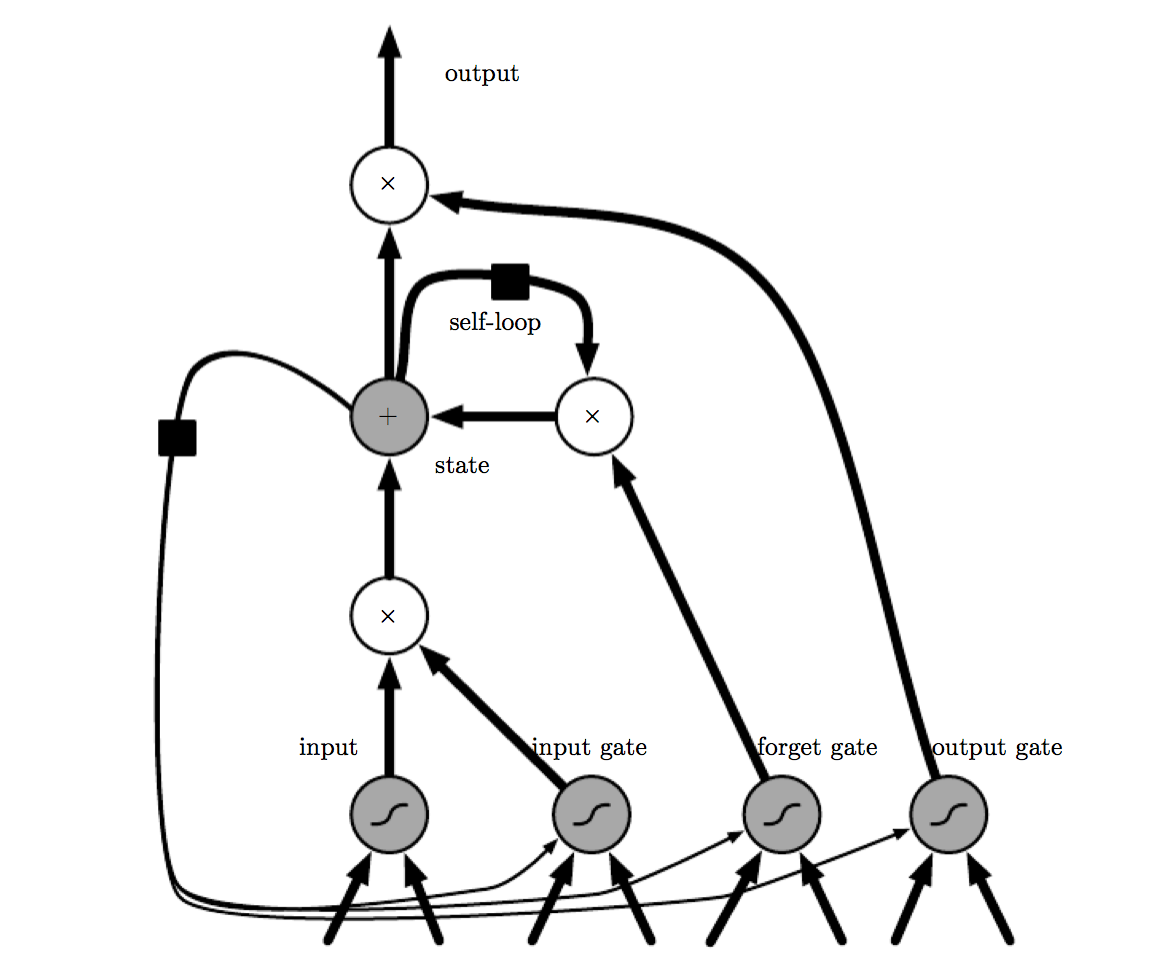
\includegraphics[width=\textwidth]{lstm}
  \caption{Estructura de la compuerta cerrada de una LSTM.
    (Tomado de \cite{goodfellow-et-al-2016})}
  \label{lstm_fig}
\end{figure}

La arquitectura RNN-LSTM se caracteriza por ser superficial en cuanto al número de neuronas que separan una\
entrada de una salida; sin embargo, ello no implica un pobre desempeño. Una \textbf{célula LSTM} contiene\
\begin{itemize}
\item un \emph{bucle} interno;
\item las mismas entradas y salidas de una RNN ordinaria;
\item una \emph{unidad de estado} $s_i^{(t)}$ que se conecta a sí misma a través del bucle,\
  de manera lineal;
\item una \emph{compuerta de olvido} $f_i^{(t)}$ que controla la matriz de pesos del bucle y\
  mantiene un valor entre 0 y 1 por medio de una activación sigmoide;
\item una \emph{compuerta de entrada} $g_i^{(t)}$ que mantiene sus valores entre 0 y 1\
  mediante una sigmoide;
\item una \emph{compuerta de salida} $q_i^{(t)}$ que mantiene sus valores entre 0 y 1\
  mediante una sigmoide.
\end{itemize}\par
Aquí hablamos de la $i$-ésima célula en el tiempo $t$. En símbolos,
\begin{align}
  f_i^{(t+1)} &= \sigma\left(b_i^f + \sum_j U_{i,j}^f x_j^{(t+1)} + \sum_j W_{i,j}^f h_j^{(t)}\right)\\
  s_i^{(t+1)} &= f_i^{(t+1)} s_i^{(t)} + g_i^{(t+1)} \nonumber \\
  &+ \sigma\left(b_i + \sum_j U_{i,j} x_j^{(t+1)} + \sum_j W_{i,j} h_j^{(t)}\right)\\
  g_i^{(t+1)} &= \sigma\left(b_i^g + \sum_j U_{i,j}^g x_j^{(t+1)} + \sum_j W_{i,j}^g h_j^{(t)}\right)\\
  h_i^{(t+1)} &= \tanh(s_i^{(t+1)}) q_i^{(t+1)}\\
  g_i^{(t+1)} &= \sigma\left(b_i^O + \sum_j U_{i,j}^O x_j^{(t+1)} + \sum_j W_{i,j}^O h_j^{(t)}\right)
\end{align}\par
donde $\mathbf{x}^{(t+1)}$ es el vector de entrada actual y $\mathbf{h}^{(t+1)}$ es el vector\
de la capa oculta actual. $\mathbf{b}$, $\mathbf{U}$ y $\mathbf{W}$ son los sesgos,\
pesos de entrada y recurrentes para la célula LSTM, respectivamente; los análogos\
que contienen algún superíndice entre $^f$, $^g$ y $^O$ corresponden a los pesos de\
las compuertas de olvido, entrada y salida, respectivamente.\par
Con estas ecuaciones, es posible realizar propagación hacia adelante sin mayor problema.\
Para entrenar una red LSTM, se puede usar una variante del algoritmo de propagación hacia\
atrás (a través del tiempo) como se proporciona en \cite{hochreiter1997}.


\chapter{Red neuronal para descripciones de memes}

\noindent
\lettrine[lines=2, lhang=0.33, loversize=0.25]{\textbf{D}}{ejando}\
de lado la teoría memética introducida por Dawkins \cite{dawkins2006}, consideraremos a\
un \emph{meme} de forma abstracta, separando su representación visual de su leyenda.\
Por consecuencia, la arquitectura neuronal que se presentará en este capítulo,\
tratará de procesar los siguientes tipos de datos:
\begin{itemize}
\item Un \emph{tensor} con dimensiones \verb+[w, h, 3]+
  \footnote{
    Aquí, usamos la notación del paquete \href{http://www.numpy.org}{NumPy}\
    del lenguaje de programación \emph{Python} para referirnos a las dimensiones\
    de un tensor.
  }, donde \verb+w+ y \verb+h+ son el ancho y el largo de una imagen, mientras que\
  el 3 simboliza los canales de la misma (RGB).
\item Un vector que contiene los índices correspondientes a las palabras de una leyenda;\
  éstos se obtienen \textit{mapeando} números naturales con un diccionario que reúne todas
  las palabras del conjunto de datos de entrenamiento.
\end{itemize}

\section{Formalización del problema de aprendizaje}

\noindent
Los recientes avances en generación de descripciones de imágenes destacan el éxito\
de una CNN que obtiene una representación vectorial de las características más\
importantes de las imágenes de entrenamiento\cite{DBLP:journals/corr/VinyalsTBE14}.\
Vinyals, \emph{et al}, además proponen canalizar estos vectores hacia una arquitectura recurrente\
que, junto con las descripciones de las mismas creen un modelo de lenguaje\
\footnote{
  Llamamos \textbf{modelo de lenguaje \textit{probabilístico}} a una distribución de\
  probabilidad sobre todos los enunciados formados por las palabras de un diccionario.\
  Un buen modelo de lenguaje debe de maximizar la \emph{probabilidad conjunta} enunciados\
  que sean coherentes sintáctica y semánticamente.
}.\par
La comunidad de procesamiento de lenguaje natural se ha \emph{inspirado} en el modelo de\
\emph{traducción automática neuronal} que incorpora una LSTM, cuya memoria inicial está dada por\
los vectores salientes de la CNN, que codifica un enunciado de entrada de longitud indefinida\
en una representación de longitud fija para, posteriormente, ``decodificar'' ésta última en\
un enunciado objetivo. Intuitivamente, se puede pensar en una máquina abstracta que, dadas las\
características de una imagen intenta ``traducir'' las palabras $S_1,\ldots,S_t$ (un prefijo\
de la imagen) para obtener el sufijo $S_{t+1},\ldots,S_{N}$.\par
Formalmente, estamos construyendo dos distribuciones de probabilidad dadas por la CNN y la LSTM,\
respectivamente. El problema, en cuestión, de aprendizaje automático consiste en maximizar\
la \emph{verosimilitud} de la descripción correcta de una imagen $I$ por un enunciado $S$:
\begin{equation}
  \theta^* = \argmax_\theta \sum_{I, S} \log p(S|I;\theta)
\end{equation}
donde $\theta$ son los parámetros del modelo. En este caso, $S$ representa a cualquier enunciado\
sin restricción de longitud; para fijar su longitud, hacemos uso de la regla de la cadena\
probabilística para calcular la $\log$-probabilidad de $S = S_0,\ldots,S_N$:
\begin{equation}
  \log p(S|I) = \sum_{t=0}^N \log p(S_{t+1}|I,S_0,\ldots,S_t).
\end{equation}
Obsérvese que la dependencia de los parámetros $\theta$ continúa aunque no se haga explícito.\par
En otras palabras, proponemos usar una LSTM para estimar $p(S_{t+1}|I,S_0,\ldots,S_t)$, de acuerdo\
al \emph{estado del arte} actual de tareas de predicción de secuencias de símbolos. La tupla\
$(I,S)$, será uno de los tantos ejemplares de entrenamiento, donde la imagen $I$ son las características\
encontradas por una CNN ajustadas a un espacio vectorial. Este esquema neuronal garantiza\
un aprendizaje \emph{de punto a punto}, es decir, la red tendrá la capacidad de considerar cada pixel\
de una imagen para determinar qué tanto contribuye en la generación de enunciados.

\section{Inception \emph{v.3}}

\begin{center}
  \emph{¿Cuántas capas son necesarias y suficientes?}
\end{center}\par
\noindent
Nos referimos a una CNN como \textbf{incrustadora} o \textbf{encajadora} (\emph{embedder} en inglés)\
pues su trabajo consiste en extraer las características de una imagen y comprimirlas en un espacio\
vectorial fijo. Sabemos, a partir del capítulo anterior, de la capacidad de filtrar detalles de una\
capa convolucional; sin embargo no existe pista alguna que nos muestre con exactitud qué hay que\
tomar en cuenta de un conjunto de imágnes de entrenamiento (¡y sobre todo de memes!).\par
Este problema se reduce al de la construcción de una arquitectura suficientemente \emph{general} que\
sea capaz de filtrar hasta el más mínimo detalle de una imagen. Con el fin de atacarlo,\
surgió la competencia anual \emph{``Large Scale Visual Recognition Challenge''} (ILSVRC), cuyo\
objetivo ha sido el de mejorar en la tarea general de etiquetamiento de imágenes. Aunado a ello, el laboratorio\
de visión computacional de Stanford University comparte el conjunto de datos \emph{ImageNet} que reúne\
14,197,122 imágenes etiquetadas para el entrenamiento y la evaluación de los algoritmos participantes.\par
En 2014, los modelos neuronales de gran profundidad comenzaron a ganar popularidad en esta tarea, sobre\
todo por el desempeño de la arquitectura \textbf{Inception} \cite{DBLP:journals/corr/SzegedyVISW15}.\
A diferencia de algunas de sus predecesoras (GoogLeNet, AlexNet, VGGNet), Inception reduce hasta 12 veces\
el número de parámetros (pesos) requeridos, garantizando un desempeño computacional más óptimo. Es decir,\
su escalabilidad le permite incorporarse a la industria de grandes bases de datos. Por ello, se ha decidido\
usar a Inception como ``incrustadora'' de imágenes.\par
Aquí, vale la pena destacar que la profundidad que posee Inception es del orden de 256 capas y que\
algunas de sus predecesoras se caracterizaban por una profundidad de al menos un orden de magnitud\
(exponencial) a ella. Sin embargo, la reducción en la amplitud promedio (número de dimensiones por capa)\
le permite remover algunos cuellos de botella de desempeño. A continuación, se presentan algunos\
de los principios de diseño de Inception.
\begin{enumerate}[label=\textbf{S.\arabic*}]
\item Dos capas contiguas, con un número de neuronas conectadas menor al promedio entre cualesquiera\
  otras, implican que la información está siendo comprimida mientras fluye hacia la capa de salida.\
  En general, se busca capturar la mayor cantidad de detalles, a través de un número considerable de\
  dimensiones en las primeras capas; por lo que, más o menos, el número de dimensiones debe reducirse\
  de a poco desde el inicio hasta el final.
\item Se prefiere incrementar el número de ``capas de activación'' por cada grupo de convoluciones-pooling,\
  pues esto revela una cantidad mayor de características y facilita el entrenamiento.
\item \label{sp-agg} Es posible realizar una operación de \emph{adición espacial}, en la cual se combinen incrustaciones\
  con dimensiones bajas. Más aún, se pueden realizar reducciones dimensionales tras alguna adición espacial\
  y previamente a una convolución, sin pérdida de información.
\item El balance entre la amplitud y la profundidad de la red neuronal contribuye directamente a la calidad\
  del desempeño de la misma. Sin embargo, ambas medidas deben de ser incrementadas en paralelo, para\
  garantizar un aumento \emph{constante} en el costo computacional de la red.
\end{enumerate}

\subsection{Factorización de convoluciones}

Reducción de dimensiones, en una red convolucional, implica reducción \emph{significativa} de parámetros (de pesos)\
por capa convolucional. Una de las técnicas usadas, primero por GoogLeNet
\footnote{
  Para más información sobre la arquitectura de \emph{GoogLeNet}, revisar \url{https://arxiv.org/abs/1409.4842}.
},
y luego adoptada por Inception consiste en \textbf{factorizar} (\emph{descomponer}) una capa CONV con un filtro\
``grande'' en varias capas CONV adyacentes que cuya suma de las dimensiones de sus respectivos filtros sea\
equivalente a la capa factorizada.\par

\begin{figure}[H]
  \centering
  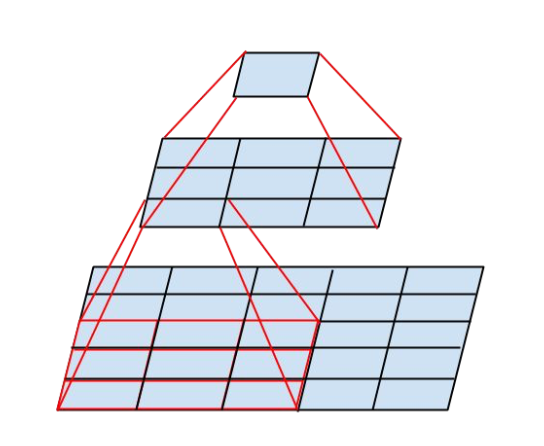
\includegraphics[width=0.6\textwidth]{conv-to-mlp}
  \caption{Una convolución de $5 \times 5$ es un perceptrón multicapa, \emph{per se}.
    (Tomado de \url{https://arxiv.org/pdf/1512.00567.pdf}.)}
  \label{conv-to-mlp}
\end{figure}

La reducción de parámetros por capa CONV implica, además, un entrenamiento más rápido. El costo radica en aplicar\
más convoluciones por cada capa CONV cuyo filtro tiene dimensiones \emph{considerablemente} grandes. Para\
profundizar más en esta idea, imaginemos un filtro de $5 \times 5$. Uno de los beneficios que trae consigo\
el tener una filtro de tamaño ``grande'' (por conveniencia, aquí así lo consideramos) es que la cobertura del\
mismo sobre una imagen le permite capturar mayores detalles de la misma. Ahora, recordemos que una capa CONV\
puede ser vista como un MLP, como se vio en el capítulo anterior; en realidad, ¡el filtro en cuestión\
es una capa totalmente conectada que pasa por toda la imagen de entrada! ¿Por qué no descomponer este MLP\
en varios filtros pequeños aplicados de manera \emph{paralela} sobre la imagen? El resultado es la\
factorización en dos filtros de $3 \times 3$ como se muestra en la figura (\ref{conv-to-mlp}).\par

\begin{figure}[H]
  \centering
  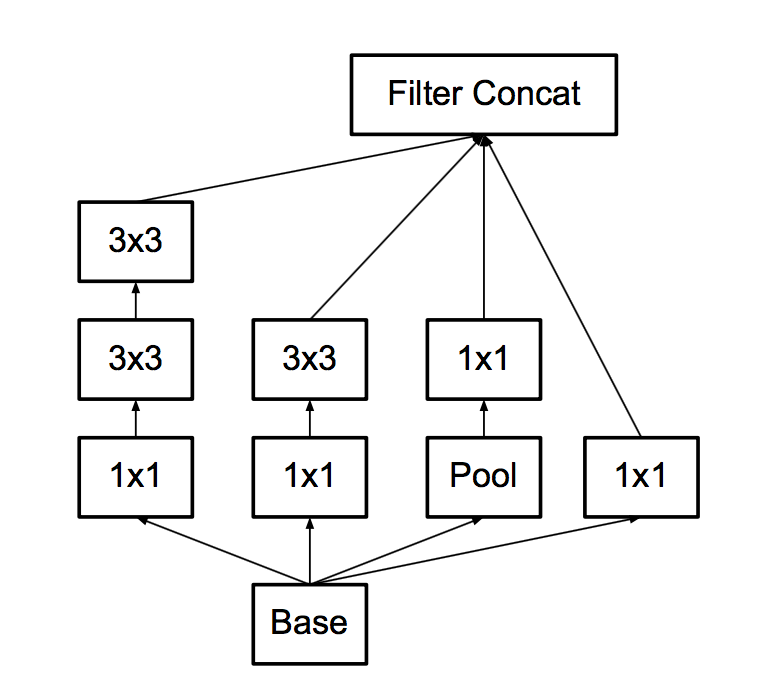
\includegraphics[width=0.6\textwidth]{factorization}
  \caption{Otra manera de factorizar una convolución consiste en paralelizar el cómputo del filtro.
    Cabe destacar que los parámetros de cada nuevo filtro son \emph{compartidos} entre sí,\
    por cada nueva capa. Aquí reemplazamos un filtro de $5 \times 5$ con dos filtros de $3 \times 3$
    y una capa de pooling.
    (Tomado de \url{https://arxiv.org/pdf/1512.00567.pdf}.)}
  \label{factorization}
\end{figure}

En términos propios de la teoría de lenguajes de programación, podemos afirmar que una red neuronal, vista como un\
lenguaje formal, posee una estructura que le permite ser construida de manera \emph{inductiva} a partir\
de pequeñas entidades \emph{bien} definidas. ¿Cómo es que, entonces, se optimiza una red CNN? Minimizando la complejidad\
del cómputo de sus estructuras básicas. En este caso, aprovechamos el cómputo paralelo para factorizar un\
filtro, de donde surgen varios ``hilos de ejecución'' en el grafo de la misma que, deberán ser\
eventualmente \emph{concatenados} en un solo tensor resultante.\par
A la estructura presentada en la figura (\ref{factorization}), se le denomina comúnmente como módulo\
\emph{Inception}. Por otro lado, decimos que una convolución con un filtro de $1 \times 1$ procesa\
\emph{localmente} una imagen de entrada pues realiza una activación (filtrado) exhaustiva a nivel\
de pixeles individuales. En contraste, siguiendo el principio de diseño (\ref{sp-agg}), la reducción\
una adición espacial incorpora dos o más entradas en una. La reducción de dimensiones toma un papel\
clave para garantizar que no haya pérdida de información. No obstante, un incremento en tasa de procesamientos\
locales contra adiciones espaciales favorece la existencia de representaciones dispersas de dimensiones\
altas.

\begin{figure}[H]
  \centering
  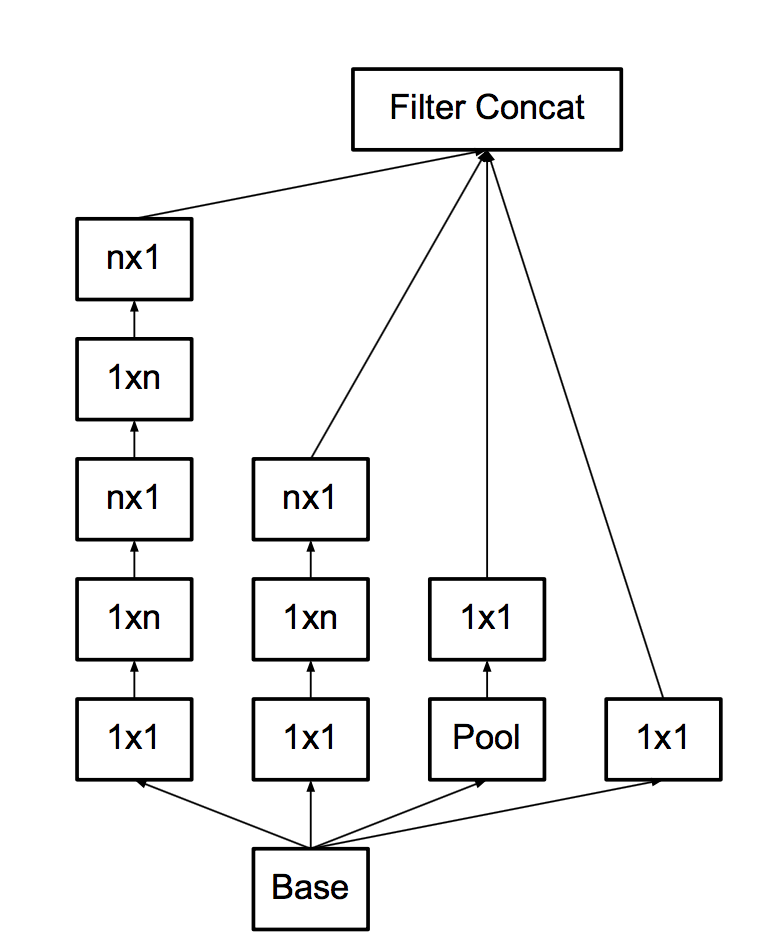
\includegraphics[width=0.6\textwidth]{factorization2}
  \caption{Factorización de una convolución de $n \times n$, donde $n = 7$.
    (Tomado de \url{https://arxiv.org/pdf/1512.00567.pdf}.)}
  \label{factorization2}
\end{figure}

\begin{figure}[H]
  \centering
  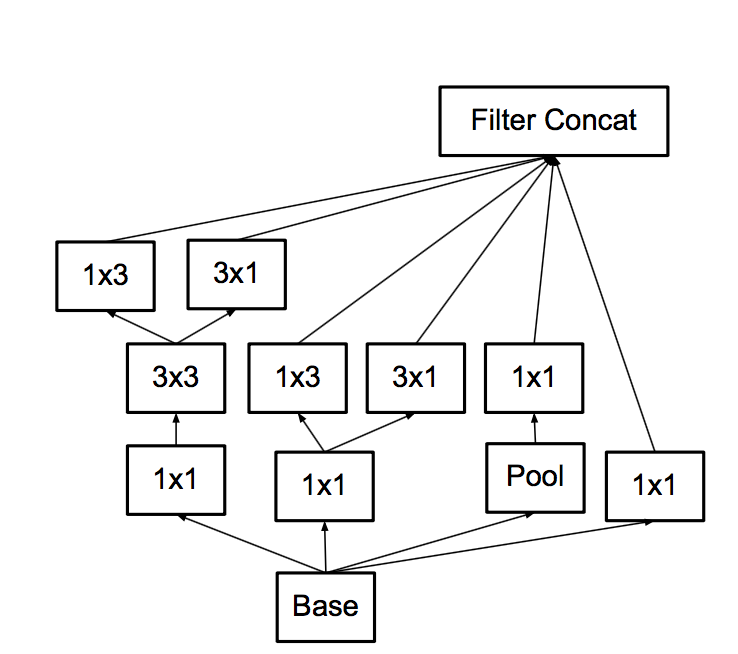
\includegraphics[width=0.6\textwidth]{factorization3}
  \caption{Factorización de una convolución de $8 \times 8$.
    (Tomado de \url{https://arxiv.org/pdf/1512.00567.pdf}.)}
  \label{factorization3}
\end{figure}

Para concluir con esta sección, presentamos las capas que constituyen a la arquitectura Inception\
en la siguiente tabla.

\noindent
\resizebox{\textwidth}{!}{
  \begin{tabular}{|l|c|c|}
    \hline
    \textbf{tipo} & \textbf{tamaño de filtro / zancada} & \textbf{tamaño de la entrada}\\
    \hline \hline
    CONV & $3 \times 3 / 2$ & $299 \times 299 \times 3$ \\
    \hline
    CONV & $3 \times 3 / 1$ & $149 \times 149 \times 32$ \\
    \hline
    CONV con relleno de ceros & $3 \times 3 / 1$ & $147 \times 147 \times 32$ \\
    \hline
    POOL & $3 \times 3 / 2$ & $147 \times 147 \times 64$ \\
    \hline
    CONV & $3 \times 3 / 1$ & $73 \times 73 \times 64$ \\
    \hline
    CONV & $3 \times 3 / 2$ & $71 \times 71 \times 80$ \\
    \hline
    CONV & $3 \times 3 / 1$ & $35 \times 35 \times 192$ \\
    \hline
    $3 \times$ Inception & figura (\ref{factorization}) & $35 \times 35 \times 288$ \\
    \hline
    $5 \times$ Inception & figura (\ref{factorization2}) & $17 \times 17 \times 768$ \\
    \hline
    $2 \times$ Inception & figura (\ref{factorization3}) & $8 \times 8 \times 1280$ \\
    \hline
    POOL & $8 \times 8 / 2$ & $8 \times 8 \times 2048$ \\
    \hline
    LINEAL & logits ($\log$-probabilidades) & $1 \times 1 \times 2048$ \\
    \hline
    MLP-SOFTMAX & clasificador & $1 \times 1 \times 1000$ \\
    \hline
  \end{tabular}
}

\section{Poniendo todo junto}

\noindent
Esencialmente, la estructura de cada unidad LSTM usada en la implementación de la RNN es la misma\
que la que fue presentada en la última sección del capítulo anterior. Lo único que cambia es la\
incorporación del tensor de la penúltima capa de Inception ($CNN(I)$), como memoria inicial ($h^{(0)}$).\par
El entrenamiento de la LSTM se lleva a cabo \emph{desenvolviendo} la recurrencia en un tamaño\
fijo de copias de la LSTM (digamos, $N$). En el tiempo $t+1$, se calcula la probabilidad que tiene\
cada palabra en el diccionario de ser $S_{t+1}$ a partir de $p(S_t|I,S_0,\ldots,S_{t-1})$.\
En resumen,
\begin{align}
  x_{-1} &= CNN(I)\\
  x_t &= W_eS_t,\ \ t \in \{0,\ldots,N-1\}\\
  p_{t+1} &= LSTM(x_t),\ \ t \in \{0,\ldots,N-1\}
\end{align}
donde $x_{-1}$ indica la primera entrada de la LSTM, $x_t$ son las entradas subsecuentes,
$W_e$ es un tensor que incrusta la palabra $S_t$ en el mismo espacio vectorial que $CNN(\cdot)$ y\
$p_{t+1}$ es el tensor de $\log$-probabilidades por cada palabra en el diccionario en el tiempo $t+1$.\
Cabe destacar que $S_t$ se representa matricialmente como un vector codificado \emph{en caliente}
\footnote{
  En una codificación \textbf{en caliente} (\emph{one-hot encoding}, en inglés), se aplica la\
  función indicadora sobre un vector con la dimensión del diccionario de palabras, dejando un 1\
  en el índice que corresponde a la palabra $i$ y 0 en cualquier otro.
}.\par
El error de la arquitectura se calcula mediante la verosimilitud logarítmica negativa,\
sumando cada palabra:
\begin{equation}
  L(I, S) = - \sum_{t=1} ^N \log p_t(S_t). 
\end{equation}
Acto seguido, se minimiza este error con respecto a todos los parámetros de la LSTM, la penúltima\
capa de la CNN y las incrustaciones $W_e$.\par
Finalmente, para la generación de enunciados se utiliza el algoritmo de \textbf{búsqueda por haces}\
(\emph{beam search} en inglés). Iterativamente, se considera el conjunto de las $k$ mejores palabras\
que son candidatas para ser $S_t$ en el tiempo $t$. Esto es una aproximación de
\begin{equation}
  S = \argmax_{S'} p(S'|I)
\end{equation}

\begin{figure}[H]
  \centering
  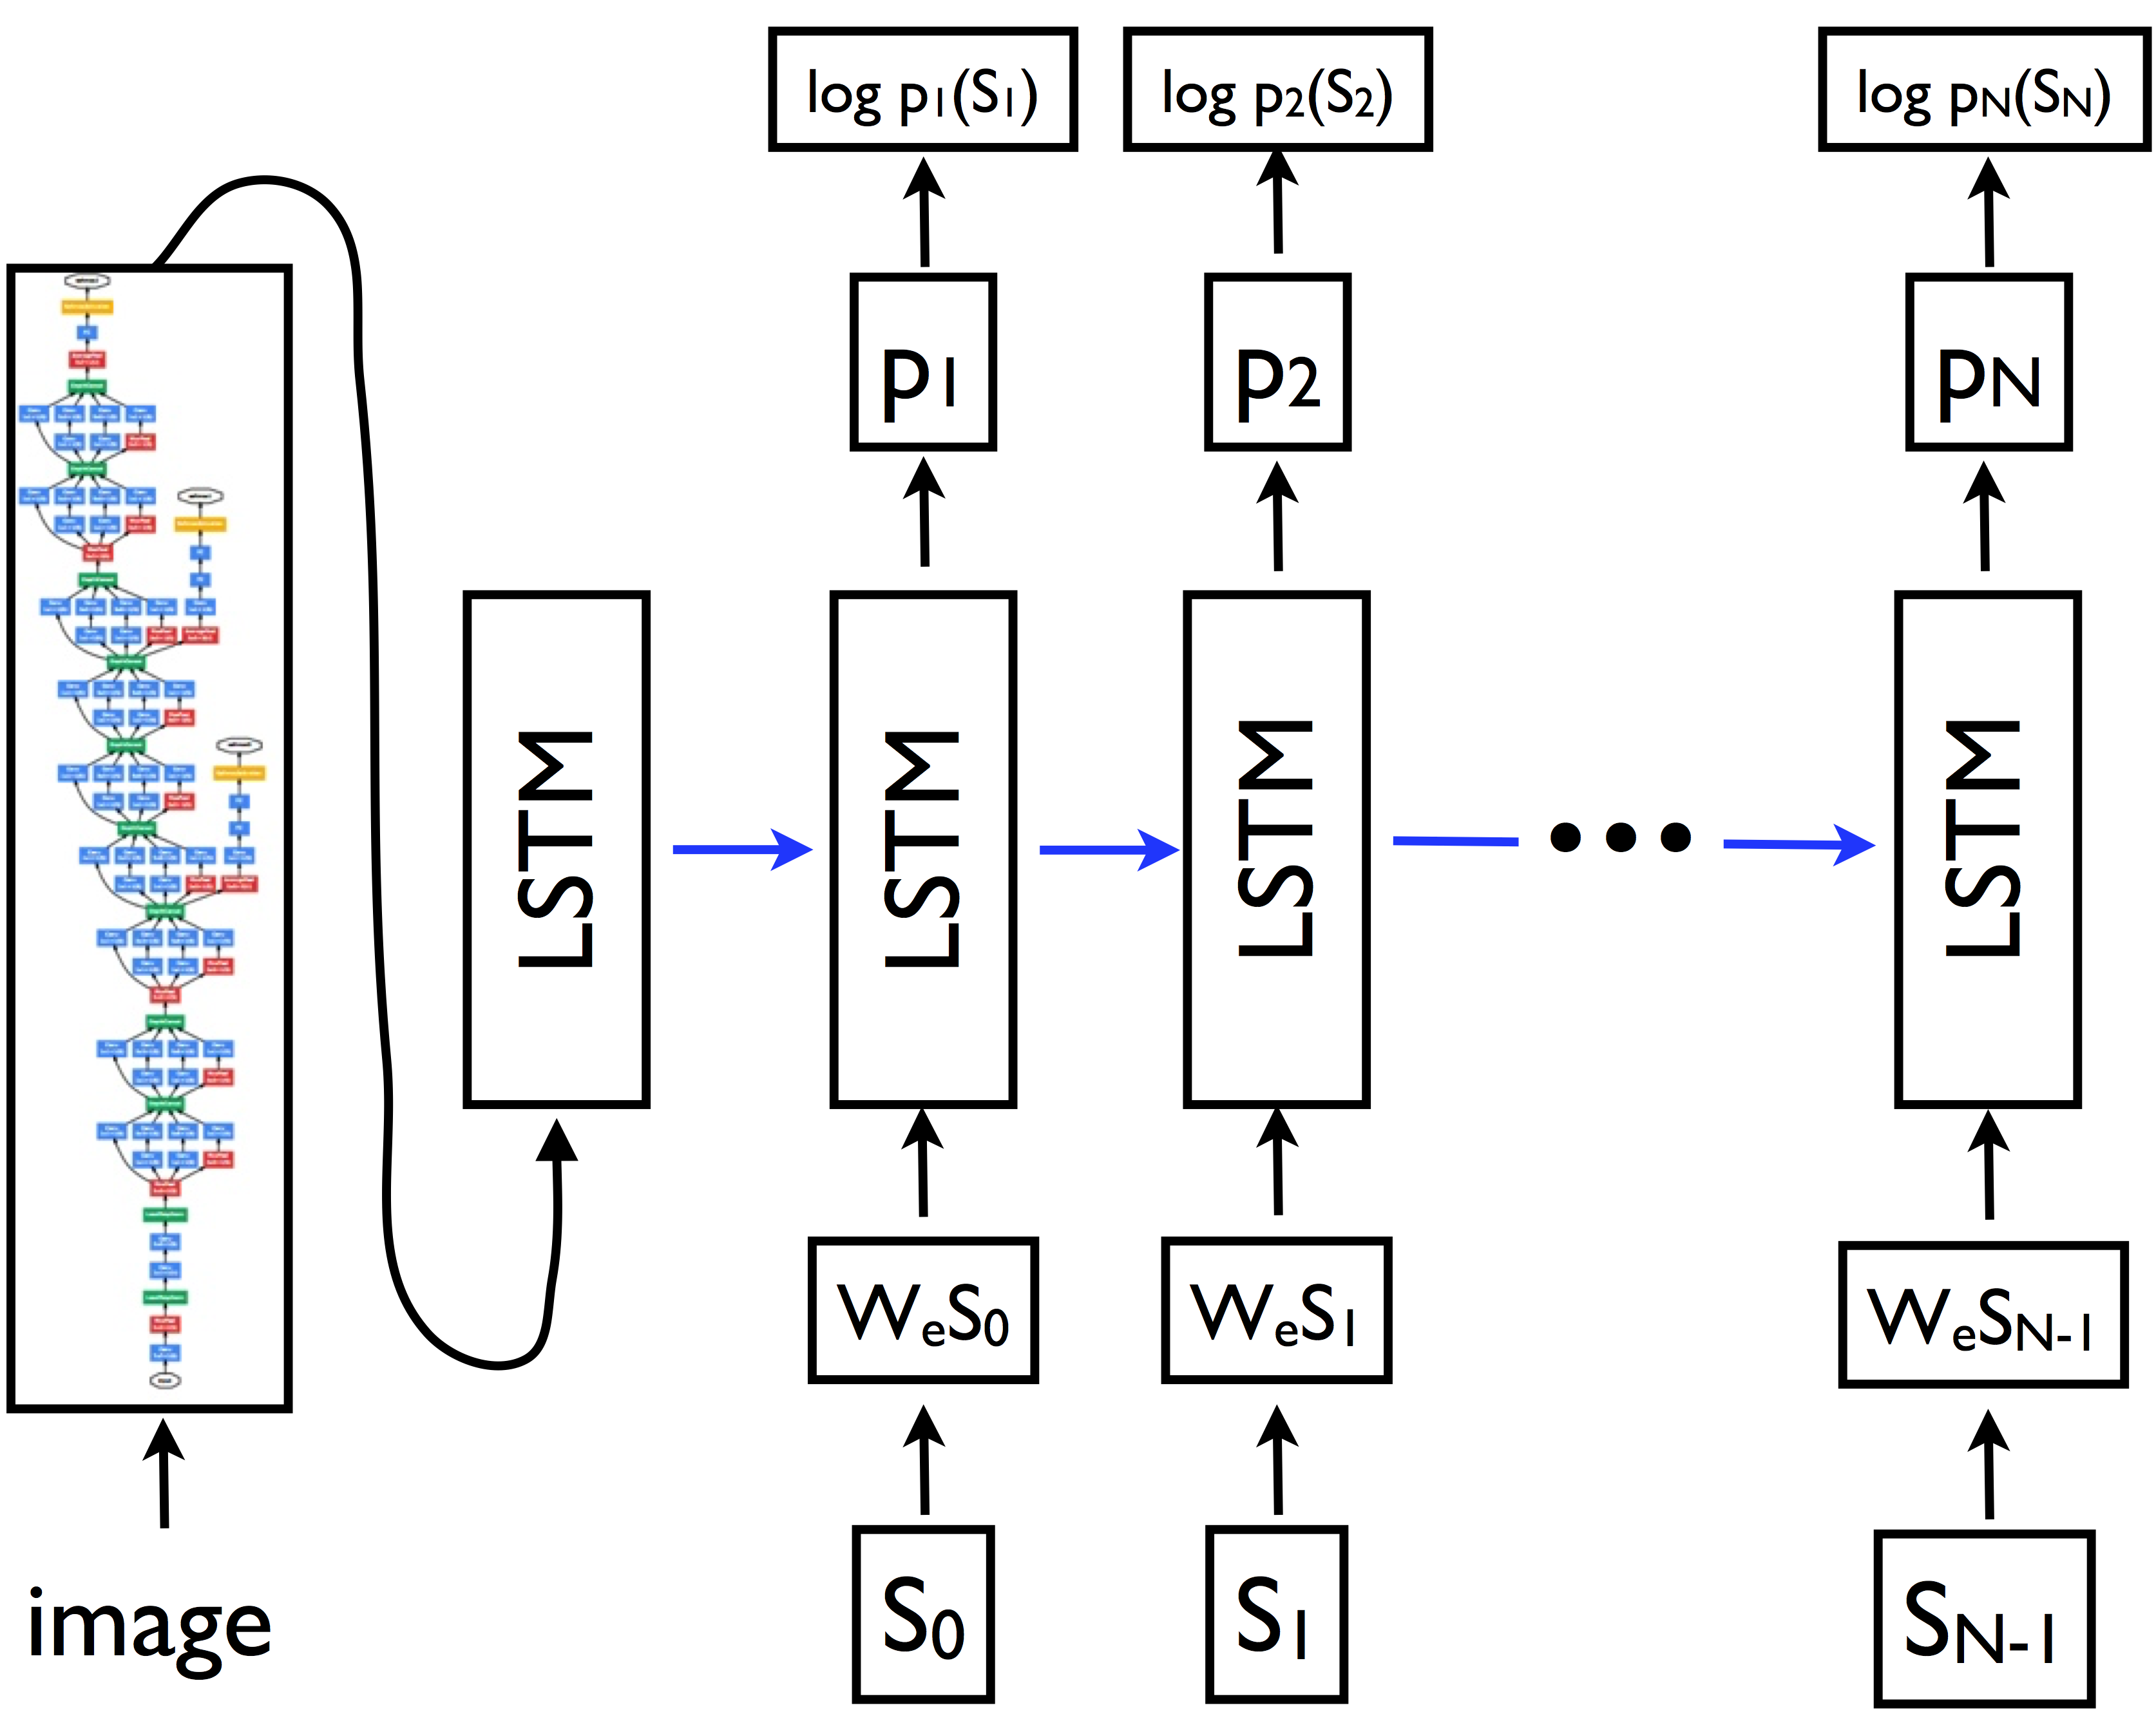
\includegraphics[width=0.9\textwidth]{show_and_tell_architecture}
  \caption{La arquitectura \emph{Show and Tell}, propuesta por Vinyals, \emph{et al},\cite{DBLP:journals/corr/VinyalsTBE14}
    en la cual se conecta una CNN Inception con una LSTM.
    (Tomado de \url{https://arxiv.org/pdf/1411.4555.pdf}.)}
  \label{show_and_tell_architecture}
\end{figure}

\chapter{Experimentación y evaluación del desempeño de la red}
\chaptermark{Experimentación y evaluación}

\noindent
\lettrine[lines=2, lhang=0.33, loversize=0.25]{\textbf{E}}{n}\
este capítulo se detallarán los experimentos hechos con la arquitectura expuesta\
anteriormente. La metodología llevada a cabo consistió en reunir la mayor cantidad\
posible de datos para seguir con los procedimientos descritos en la Sección \ref{sec:arq-accion}.\
Los alcances de los experimentos serán descritos más adelante, dejando en claro\
las restricciones de tiempo (para la realización de la tesis) y capacidad de equipo\
de cómputo disponible.\par
Con respecto a lo último mencionado, para los cómputos de mayor desempeño se utilizó una\
\textbf{tarjeta gráfica} (\emph{GPU}, por sus siglas en inglés) \emph{GeForce GTX 1080 Ti}\
de la marca \emph{NVIDIA}\footnote{
  Para mayor información con respecto al modelo \emph{GeForce GTX 1080 Ti},\
  consultar el sitio \url{http://la.nvidia.com/graphics-cards/geforce/pascal/la/gtx-1080-ti}.
}. Es común que en aprendizaje profundo se usen este tipo de componentes, que originalmente\
se construyen para el mundo de los videojuegos.

\section{Estructura del conjunto de datos} \label{sec:dataset}

\noindent
Como ya fue mencionado anteriormente, los datos se obtuvieron del sitio \verb+MemeGenerator.net+%
\footnote{\url{https://memegenerator.net}}.\
La información recabada en este sitio es reunida a través de usuarios alrededor del mundo,\
quienes de manera libre tienen la posibilidad de generar un nuevo meme. El sitio, además,\
agrupa a los memes en personajes (Figura \ref{meme-characters}) y los jerarquiza en base a\
su popularidad%
\footnote{
  Más aún, cualquier usuario puede crear libremente un personaje nuevo, lo que habilita la idea de\
  buscar y agrupar los memes de acuerdo a su personaje.
}.\par
En total se reunieron \textbf{4379} personajes del sitio web antes mencionado. Por cada uno de ellos\
el número de leyendas usadas para entrenar varía según los resultados obtenidos en cada experimento.\
Considerando que es necesario dividir un conjunto de datos en subconjuntos de entrenamiento y\
validación%
\footnote{
  Usualmente esta división se realiza muestreando aleatoriamente del $70$ al $80\%$ de los datos\
  para entrenamiento y del $30$ al $20\%$ para validación.
}, podemos afirmar que el tamaño de los datos de entrenamiento es pequeño en relación a otros\
conjuntos como \emph{ImageNet}.

\begin{figure}[h]
  \centering
  \begin{minipage}[l]{0.3\linewidth}
    
\includegraphics[width=\linewidth]{meme1}
  \end{minipage}\hfill
  \begin{minipage}[r]{0.3\linewidth}
    
\includegraphics[width=\linewidth]{meme2}
  \end{minipage}\hfill
  \begin{minipage}[r]{0.3\linewidth}
    
\includegraphics[width=\linewidth]{meme3}
  \end{minipage}
  \begin{minipage}[r]{0.3\linewidth}
    
\includegraphics[width=\linewidth]{meme4}
  \end{minipage}\hfill
  \begin{minipage}[r]{0.3\linewidth}
    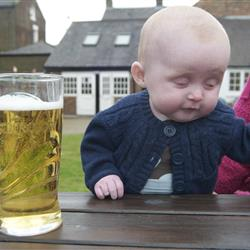
\includegraphics[width=\linewidth]{meme5}
  \end{minipage}\hfill
  \begin{minipage}[r]{0.3\linewidth}
    
\includegraphics[width=\linewidth]{meme6}
  \end{minipage}
  \begin{minipage}[r]{0.3\linewidth}
    
\includegraphics[width=\linewidth]{meme7}
  \end{minipage}\hfill
  \begin{minipage}[r]{0.3\linewidth}
    
\includegraphics[width=\linewidth]{meme8}
  \end{minipage}\hfill
  \begin{minipage}[r]{0.3\linewidth}
    
\includegraphics[width=\linewidth]{meme9}
  \end{minipage}
  \caption{
    Ejemplos de personajes populares del sitio \url{https://memegenerator.net}.
    La mayoría de ellos gozaba de gran popularidad entre los años 2009 y 2013;
    la evolución de la viralidad de los mismos y el surgimiento de otros sitios web
    para compartir memes son algunas causas que pueden explicar su ``extinción''.
    (Tomado de \url{https://memegenerator.net}.)
  }
  \label{meme-characters}
\end{figure}

Mediante una búsqueda \emph{por profundidad}, a través del árbol de páginas web, definido por cada uno de los personajes\
del sitio, uno encuentra una gran cantidad de leyendas separadas de la imagen de su personaje asociado.\
Es decir, por cada personaje se extrae una imagen y tantas leyendas como sea posible (Figura \ref{meme-separation}).\par
Para llevar a cabo este fin, se programó un \textbf{rastreador web} (\emph{web crawler}) para llevar a cabo\
la búsqueda de la información y la acumulación de los datos. Se escribió un programa en el lenguaje de\
programación \textbf{Python} (versión 3.6)\footnote{\url{https://www.python.org}} con la biblioteca\
\textit{Scrapy} (versión 1.4.0)\footnote{\url{https://scrapy.org}}, la cual organiza hilos de ejecución concurrentes\
para obtener el contenido de las \verb+URL+'s necesarias mediante peticiones \verb+GET+ de \verb+HTTP+.\
Al final, se organizaron los datos bajo la jerarquía presente en la Figura \ref{file-hierarchy}.

\begin{figure}[h]
  \centering
  \begin{minipage}[l]{\linewidth}
    \dirtree{%
      .1 personaje-1/.
      .2 personaje-1{.}csv.
      .2 personaje-1{.}jpg.
      .2 personaje-1-metadata{.}csv.
      .1 personaje-2/.
      .2 personaje-2{.}csv.
      .2 personaje-2{.}jpg.
      .2 personaje-2-metadata{.}csv.
      .1 {.}.
      .1 {.}.
      .1 {.}.
      .1 personaje-n/.
      .2 personaje-n{.}csv.
      .2 personaje-n{.}jpg.
      .2 personaje-n-metadata{.}csv.
    }
  \end{minipage}
  \caption{
    Como se observa, los datos se guardaron bajo el formato \texttt{CSV}, asociando cada leyenda con la \texttt{URL}
    de su meme asociado y su idioma de origen (Figura \ref{meme-file}). Se estima que un $90\%$ de datos está en inglés.
  }
  \label{file-hierarchy}
\end{figure}

\begin{figure}[H]
  \centering
  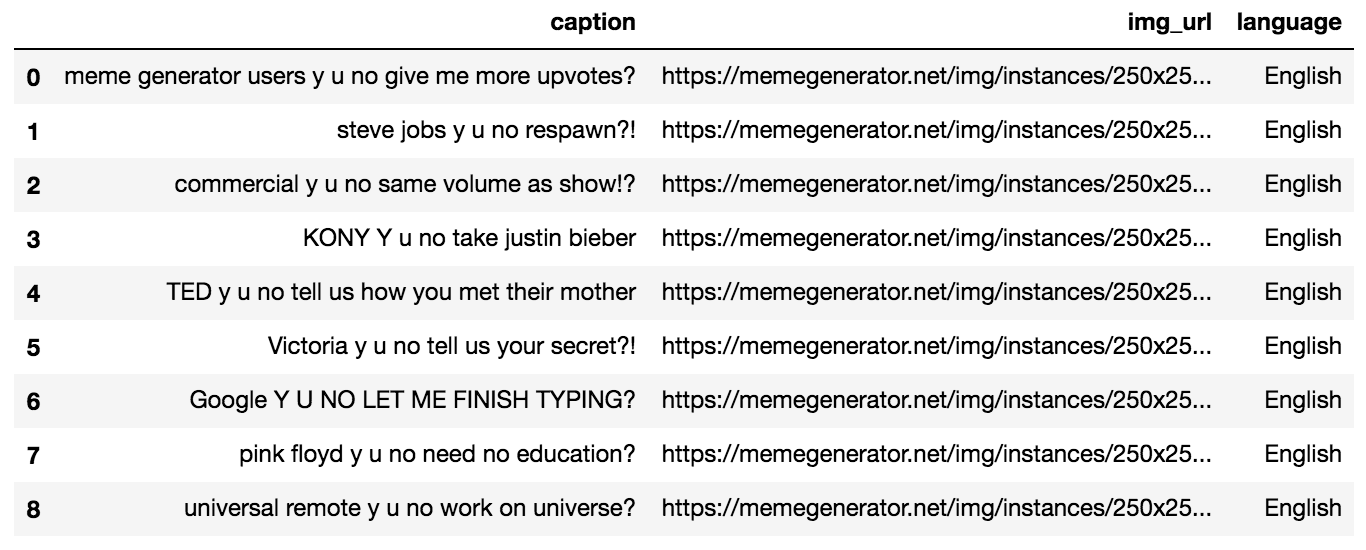
\includegraphics[width=\textwidth]{meme-file}
  \caption{
    De esta manera se guardaron cada una de las leyendas de cada personaje.
  }
  \label{meme-file}
\end{figure}

\begin{figure}
  \centering
  \begin{minipage}[l]{\linewidth}
    
\includegraphics[width=\linewidth]{thesis-i-demand-trial-by-combat}
  \end{minipage}\hfill
  \begin{minipage}[r]{0.5\linewidth}
    
\includegraphics[width=\linewidth]{tyrionlannister}
  \end{minipage}\hfill
  \begin{minipage}[r]{0.5\linewidth}
    \verb+thesis  i demand trial by combat+
  \end{minipage}
  \caption{
    La ilustración de la parte superior constituye a un meme que integra a un personaje con su leyenda y
    es el objeto que se propaga a través de Internet. Los datos que se reunieron se separaron como se
    indica en la ilustración de la parte inferior.
    (Tomado de \url{https://memegenerator.net}.)
  }
  \label{meme-separation}
\end{figure}

\section{Generación de leyendas}

\noindent
El modo \verb+inferencia+ del modelo consiste en generar una leyenda para una imagen de entrada.\
Dada la manera con la cual se representa el modelo de lenguaje aprendido del conjunto de datos\
de entrenamiento, sabemos que por cada palabra hay una distribución de probabilidad que evalúa\
qué tan viable es que cada palabra del vocabulario sea la que sigue. Por lo tanto, muchas veces\
conviene observar los $k$ enunciados que \emph{mejor} describen una imagen, maximizando la\
probabilidad conjunta entre cada una de las palabras que los componen (en orden).\par
La \textbf{búsqueda por haces} (\emph{beam search}, en inglés) es un algoritmo que logra calcular\
enunciados de \emph{``máxima verosimimilitud''}. El procedimiento incorpora a un agente cuyo\
objetivo es encontrar el camino de mayor \emph{peso} posible en una máquina de estados, en la cual solo\
tiene conocimiento del estado actual y los pesos para llegar a los vecinos del mismo. La salida\
del algoritmo muestra los $k$ enunciados más viables para cierta imagen. El agente, entonces\
registra de manera paralela las $k$ palabras de mayor probabilidad que sucedan a la palabra anterior.\par
Normalmente, esto se programa mediante $k$ hilos de ejecución en paralelo. Cada uno se inicializa\
aleatoriamente con las $k$ palabras de inicio de mayor probabilidad. En el paso $t$, cada\
hilo vuelve a calcular los $k$ siguientes mejores estados (un total de $k^2$ estados) y, al final,\
el agente se queda con los mejores $k$ para proceder al paso $t+1$. En este caso, se consideraron\
los $k=3$ mejores enunciados para cada imagen.

\section{Experimentos}

\noindent
Los experimentos realizados obedecen a lo sugerido por la teoría presentada en los dos capítulos anteriores.\
Se buscó seguir la metodología sugerida por el \emph{estado del arte} (\cite{DBLP:journals/corr/VinyalsTBE16}).\
Por ello, se eligió trabajar con el lenguaje de programación Python (versión 3.6) y las bibliotecas\
\textbf{Tensorflow} (versión 1.3.0)\footnote{\url{https://www.tensorflow.org}} y \textbf{Keras}\
(versión 2.0.9)\footnote{\url{https://keras.io}}.\par
Ambas bibliotecas son obra \emph{reciente} de la división de código abierto de \emph{Google}.\
\emph{Tensorflow} surgió como una iniciativa para compartir la manera en que dicha empresa despliega\
sus proyectos que involucran aprendizaje profundo. El paradigma que se sigue consiste en definir un\
grafo dirigido de \emph{tensores} como nodos, en el cual fluirá la información\footnote{
  En cada nodo del grafo, se definen \emph{operaciones} (lectura y escritura de archivos, operaciones\
  matriciales, etc.) y se da la posibilidad de especificar si van a correr en un GPU, si se cuenta con uno.
}; acto seguido, se ``compila'' el modelo y se levanta una sesión para ejecutarlo. Así, \emph{Tensorflow}\
utiliza la sintaxis de \emph{Python} para construir redes neuronales en un mayor nivel.\par
Por otro lado, \emph{Keras} se define a sí misma como una interfaz de programación de aplicaciones (\emph{API})\
de alto nivel, que utiliza como motor de ejecución a \emph{Tensorflow}. Es decir, el programador es capaz\
de escribir código que defina una red neuronal y se ejecute secuencialmente. \emph{Keras}, además,\
facilita la tarea de definir un modelo profundo con una sintaxis más amigable que la de \emph{Tensorflow}\
y configura algunos \emph{hiper-parámetros} de ésta, con el fin de facilitar el prototipado de redes neuronales\
profundas.

\subsection{Experimentos exploratorios}

\noindent
Vinyals, \emph{et al} presentan tanto en \cite{DBLP:journals/corr/VinyalsTBE14} como en \cite{DBLP:journals/corr/VinyalsTBE16}\
el \emph{estado del arte} de los modelos neuronales capaces de generar descripciones a partir de imágenes.\
Por ende, el primer paso experimental consistió en replicar el entrenamiento completo, usando el conjunto de datos\
\emph{ImageNet}.\par
Utilizando pesos pre-entrenados%
\footnote{
  \emph{Tensorflow} provee un conjunto de modelos previamente entrenados bajo un subconjunto de\
  \emph{ImageNet} (\url{http://www.image-net.org/challenges/LSVRC/2012/}). Esto ahorra tiempo en la vectorización\
  de imágenes. Para mayor información, consultar el sitio\
  \url{https://github.com/tensorflow/models/tree/master/research/slim\#tensorflow-slim-image-classification-library}.
} de Inception V3, se realizó el proceso de generar un tensor de incrustaciones de las imágenes de ImageNet\
en un espacio vectorial. Acto seguido se alimentó una LSTM con dicho tensor, como memoria inicial, y se\
entrenó utilizando las leyendas asociadas a cada imagen.\par
Dentro de las ventajas consecuentes de este experimento, está el tener una implementación\
de una LSTM para ser entrenada de nuevo, con cualquier memoria inicial. El desempeño del entrenamiento\
se ilustra en la Figura \ref{exp1}. Es importante destacar que, dadas las altas dimensiones con las que\
se trabaja en cada capa, se estima que se requieren alrededor de 1 millón de épocas para que el error\
dado por la entropía cruzada se estabilice en un valor mínimo (este comportamiento es común para la mayoría\
de los experimentos subsecuentes).\par
El objetivo principal de este primer experimento era familiarizarse con el uso de las implementaciones y la\
tecnología necesaria para realizar aprendizaje profundo. Por ende, se decidió dejar a un lado la evaluación\
del desempeño de este modelo neuronal, mediante un conjunto de datos independiente del de entrenamiento y\
validación.

\begin{figure}[H]
  \centering
  \begin{minipage}[c]{\linewidth}
    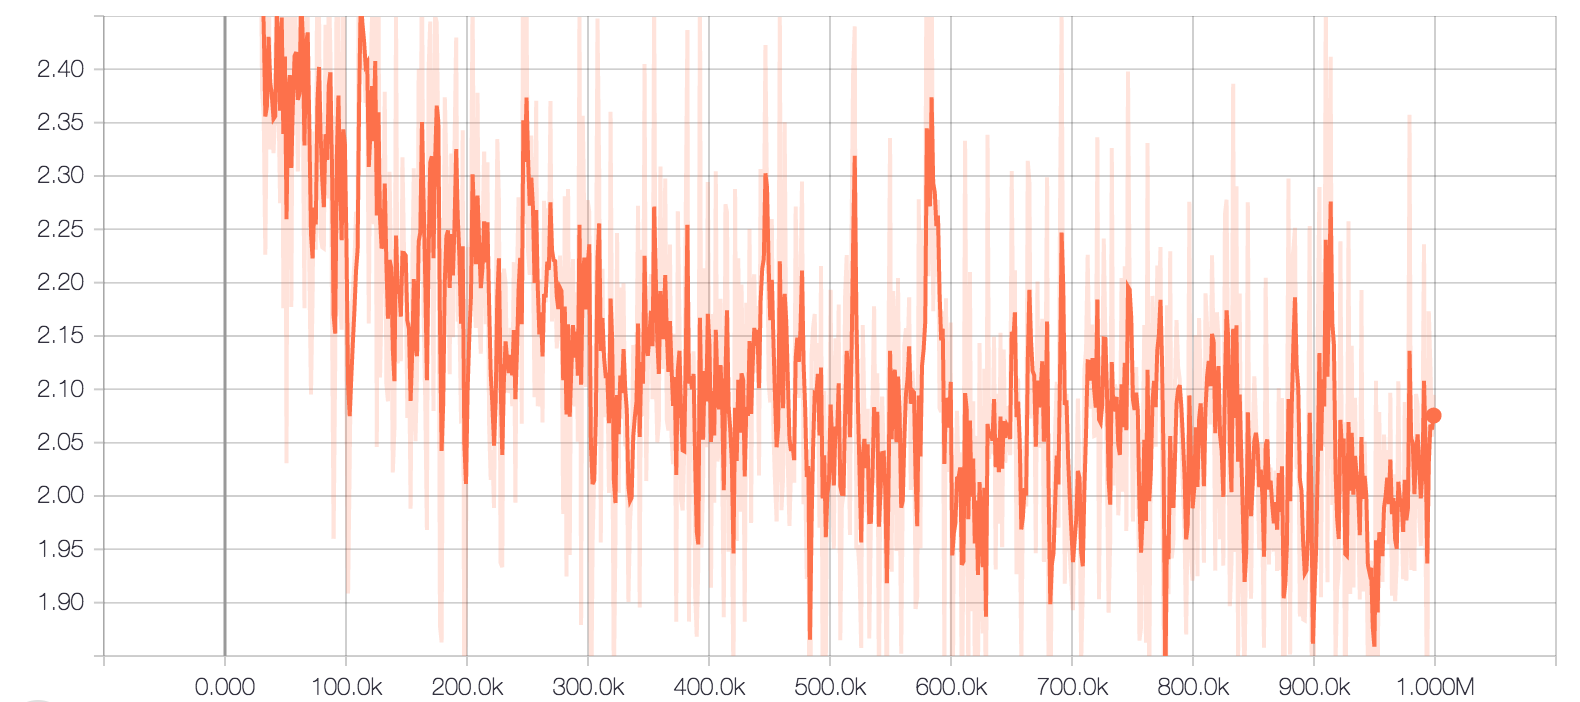
\includegraphics[width=\linewidth]{exp1-1}
  \end{minipage}\hfill
  \begin{minipage}[c]{\linewidth}
    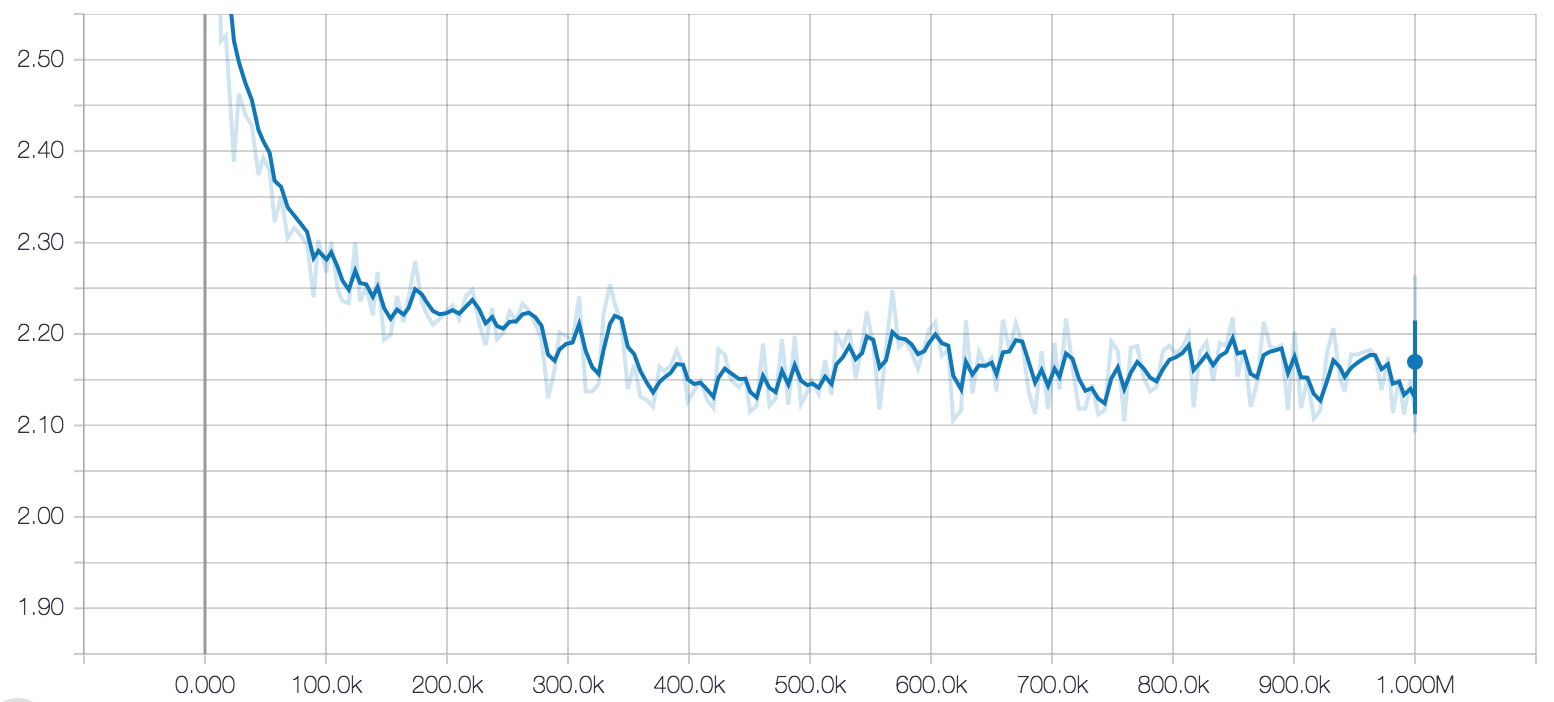
\includegraphics[width=\linewidth]{exp1-2}
  \end{minipage}
  \caption{
    Función de error de entropía cruzada para el primer experimento exploratorio.
    En el gráfico de la parte superior se muestra el error
    a través de cada época del entrenamiento, mientras que el de la parte inferior se
    calculó por medio de un conjunto de datos de \emph{validación} (de menor tamaño que el de entrenamiento).
    Ambos gráficos indican el valor de la entropía cruzada (eje de las ordenadas) a través del
    tiempo (eje de las abscisa).
    (Fuente: elaboración propia.)
  }
  \label{exp1}
\end{figure}

Tenemos, ahora, una CNN que es ``experta'' en etiquetar imágenes con detalles muy generales. Vale la pena,\
entonces, probarla con el conjunto de datos de memes. Buscamos ver, de entrada, que sea capaz de distinguir\
entre dos imágenes distintas (mediante representaciones vectoriales muy diferentes), que además se\
refleje en la discrepancia entre las leyendas generadas. Para ello, diseñamos un experimento en el\
que entrenamos una LSTM con una memoria inicial dada por los códigos convolucionales obtenidos\
a partir de \textbf{97} personajes del conjunto de datos. Estos personajes pasarán por la red\
\emph{Inception V3} pre-entrenada del experimento anterior.

\begin{figure}[h]
  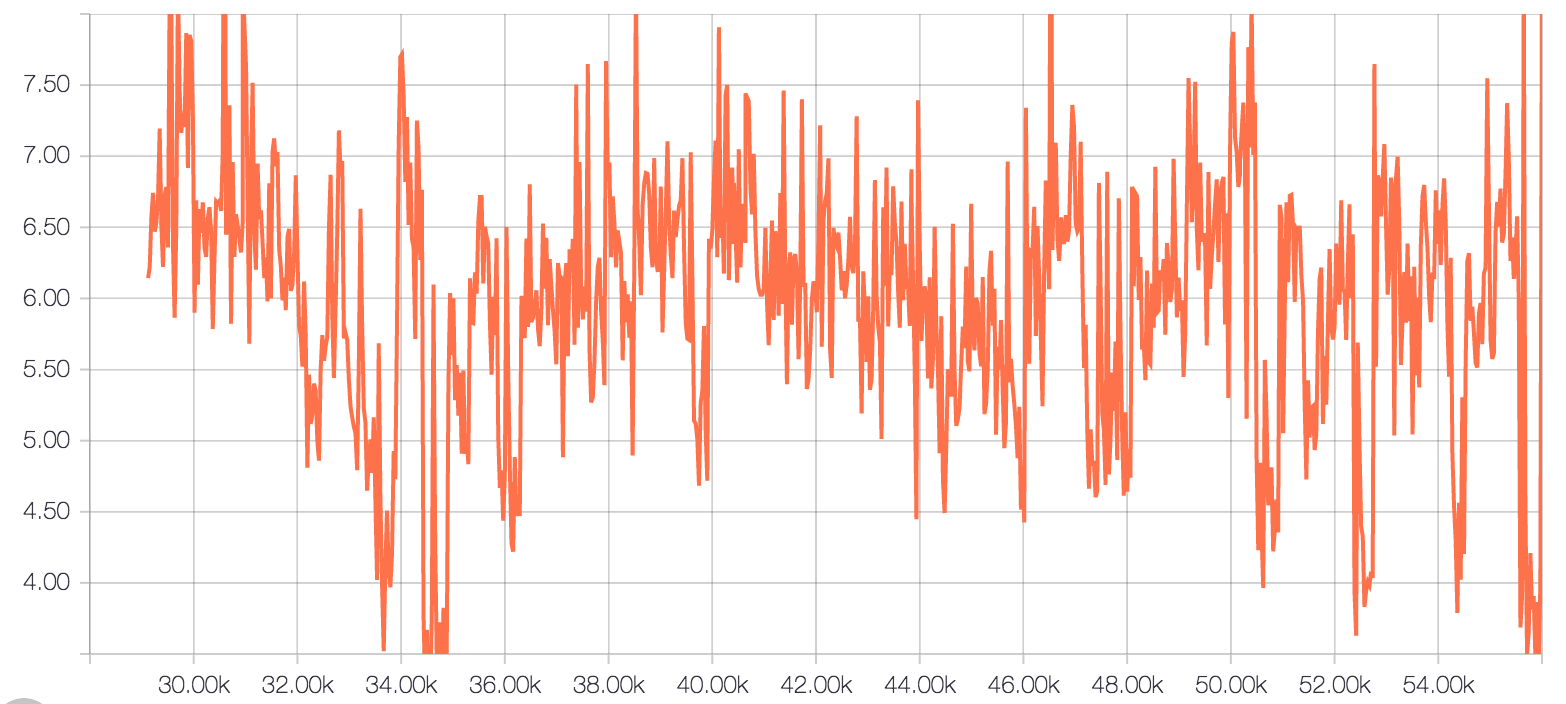
\includegraphics[width=\linewidth]{exp4-1}
  \caption{
    Función de error para el experimento que utiliza la CNN \emph{Inception V3}
    con pesos pre-entrenados, sin ser afinada.
    (Fuente: elaboración propia.)
  }
  \label{exp4}
\end{figure}

Cada personaje posee un promedio de 700 leyendas, pues el número total de leyendas por personaje varía\
según la popularidad del mismo. Cabe destacar que el vocabulario construído tuvo alrededor de 20 mil palabras distintas.\
El desempeño fue deficiente tanto en entrenamiento (Figura \ref{exp4}) como en resultados \emph{anecdóticos}.\
Las siguientes observaciones fueron notables:
\begin{itemize}
\item los códigos convolucionales resultantes del paso por la CNN fueron indistinguibles entre\
  una imagen y otra, dejando en claro la necesidad de realizar una afinación);
\item lo anterior provocó que las leyendas fueran todas iguales para imágenes distintas;
\item el elevado tamaño del vocabulario no favoreció al modelo para poder asignar probabilidades,\
  condicionales, al momento de generar frases (repetición palabras de manera contigua).
\end{itemize}\par
El bajo desempeño de este experimento motivó a \emph{no} realizar una evaluación de los resultados pero\
trajo consigo dos hipótesis para considerarse. La primera de ellas consiste en afinar la red \emph{Inception V3}\
con el conjunto de datos de memes, pues se cree que el modelo implícito en sus parámetros pre-entrenados\
explora detalles mucho más generales de los requeridos para clasificar imágenes como las mostradas en la\
Figura \ref{meme-characters}. Dado el tamaño del conjunto de datos, se plantea, de igual manera, como\
hipótesis, la viabilidad de que una CNN más \textbf{superficial} (menos profunda) tenga éxito al\
generar códigos convolucionales.

\subsection{Experimentos que involucran la afinación de una arquitectura convolucional profunda}

\noindent
Para aprovechar la especialización que posee \emph{Inception V3}, de reconocer patrones simples en\
imágenes, afinamos dicho modelo con un clasificador de memes. Dado que el conjunto de datos\
presentado en la Sección \ref{sec:dataset} no está dividido en ``categorías'' de memes, resulta difícil\
realizar una tarea de aprendizaje supervisado con una CNN.\par
Por otro lado, dadas las características de las imágenes de los memes, existe un patrón más o menos definido\
(rostro del personaje centrado en la imagen) que puede ser explotado contra la tarea general de aprender\
a clasificar \emph{ImageNet}. Esto nos brindó la solución para poder afinar a \emph{Inception V3}: colocar\
una capa MLP, al final de la red, con salida de dos dimensiones para decidir si la entrada es, o no es,\
un meme.\par
Las imágenes \emph{``no memes''} utilizadas en este punto se tomaron aleatoriamente muestreando 4379 de \emph{ImageNet}.\
Se trabajó bajo la premisa de que la profundidad de la red\
alcanzará para generalizar la identificación de las características presentes en un meme. Después de todo,\
nuestro conjunto de datos posee imágenes de mucho menor complejidad que las existentes en \emph{Inception V3}.
En total, se dejaron 3065 imágenes (memes y no memes) para entrenamiento, 657 para validación y 657 para evaluación;
el resultado de este proceso se ilustra en la Figura \ref{exp2}. El desempeño fue bastante favorable,\
ya que se minimizó considerablemente el error de la entropía cruzada. Además, con el conjunto de\
evaluación se corroboró dicho rendimiento mediante los gráficos de las métricas de \emph{precisión}%
\footnote{
  La \textbf{precisión} (\emph{accuracy}, en inglés) puede ser entendida como el porcentaje\
  de aciertos que tiene el modelo al intentar predecir un lote de datos. Se busca, entonces,\
  que su valor esté muy cercano a 1.
} y \emph{error medio absoluto}%
\footnote{
  El \textbf{error medio absoluto} es la diferencia promedio que existe entre los valores\
  estimados por un modelo ($\hat{Y}$) y los valores reales de un conjunto de datos ($Y$). Esto\
  se calcula con la expresión
  \[\frac{\sum_{i=1}^n \hat{Y}_i - Y_i}{n}.\]
} (Figura \ref{eval:exp2}).

\begin{figure}[h]
  \begin{minipage}[c]{\linewidth}
    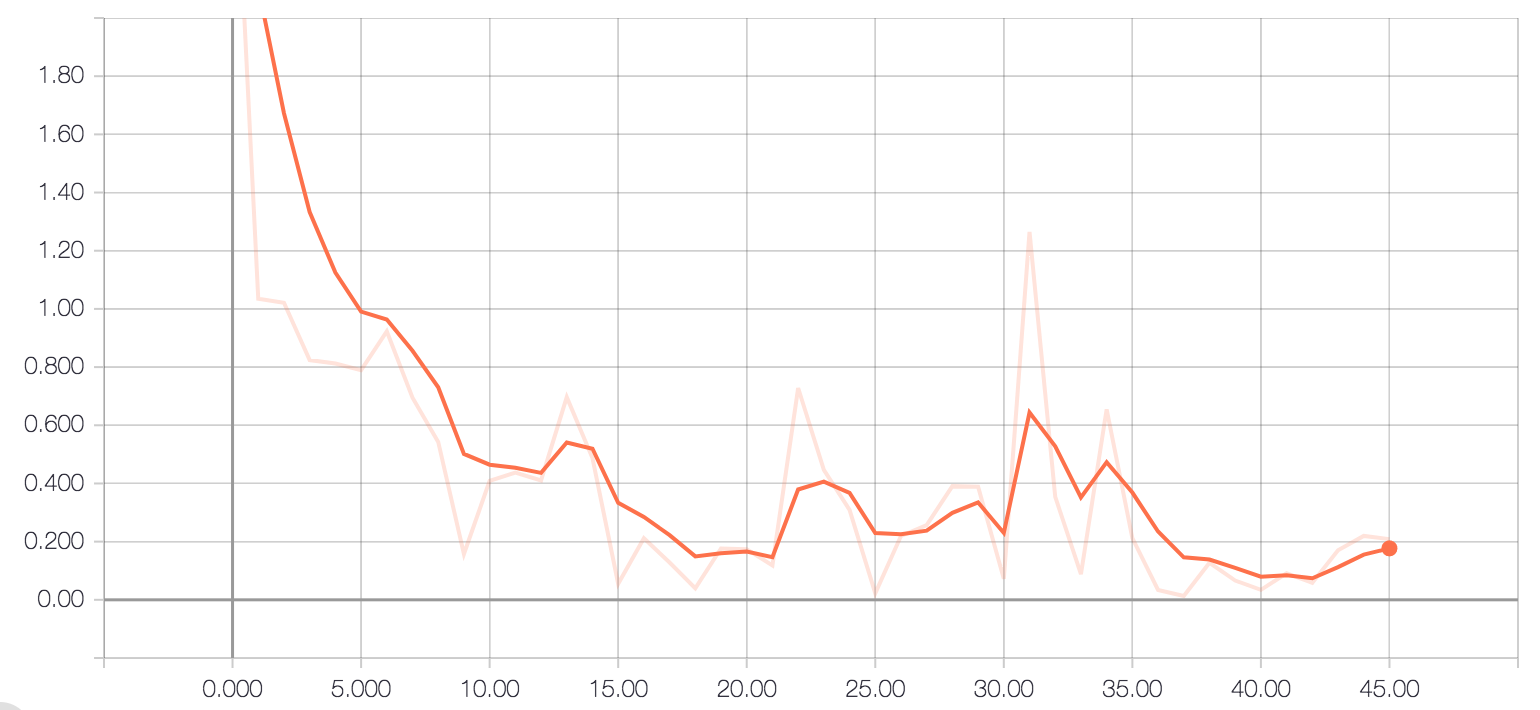
\includegraphics[width=\linewidth]{exp2-1}
  \end{minipage}\hfill
  \begin{minipage}[c]{\linewidth}
    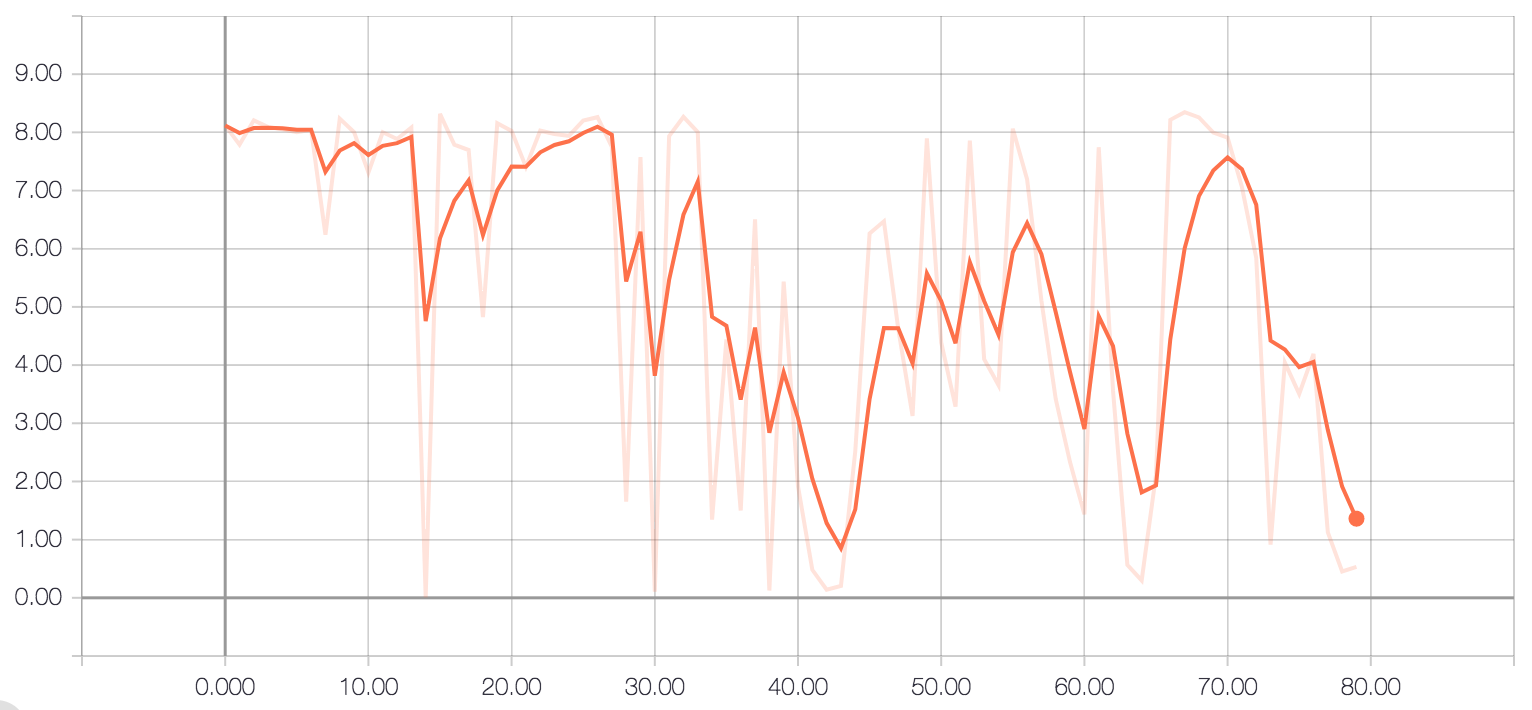
\includegraphics[width=\linewidth]{exp2-2}
  \end{minipage}
  \caption{
    Funciones de error de entrenamiento y validación (gráfico de arriba y de abajo,
    respectivamente) para la afinación de \emph{Inception V3}.
    Esto es, entrenar un clasificador entre lo que es un meme y lo que no es. Se quita\
    la última capa y se añade un MLP con dos dimensiones de salida.
    (Fuente: elaboración propia.)
  }
  \label{exp2}
\end{figure}

\begin{figure}[H]
  \centering
  \begin{minipage}[c]{\linewidth}
    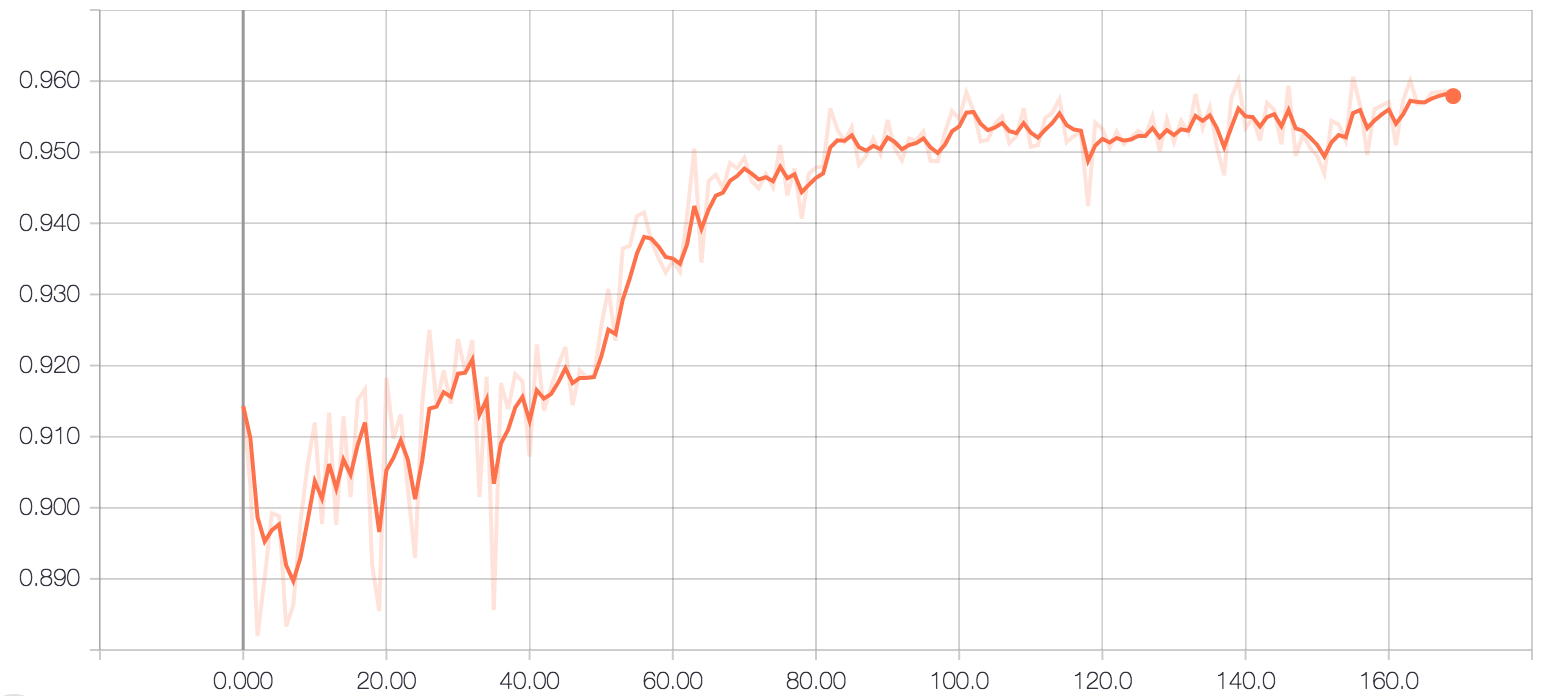
\includegraphics[width=\linewidth]{exp2-3}
  \end{minipage}\hfill
  \begin{minipage}[c]{\linewidth}
    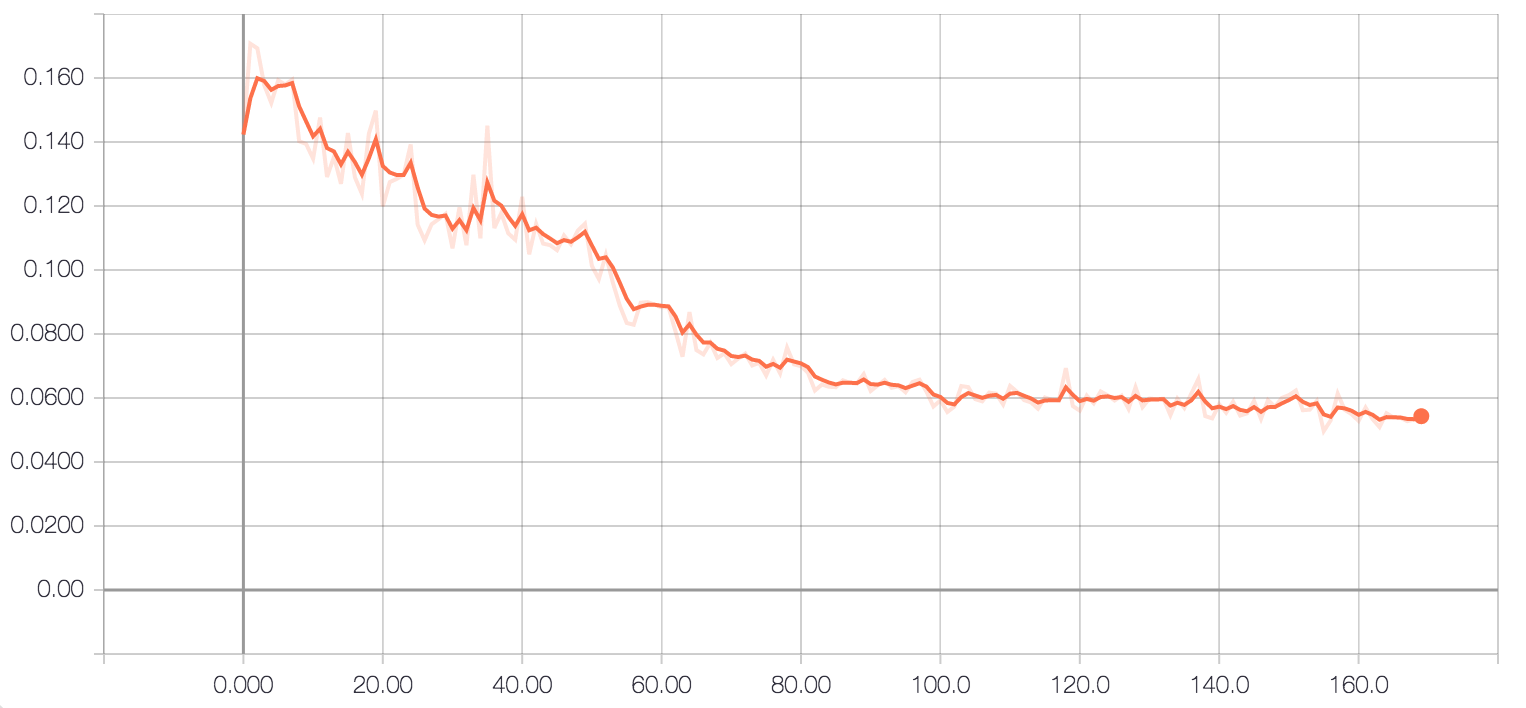
\includegraphics[width=\linewidth]{exp2-4}
  \end{minipage}
  \caption{
    Dos funciones de evaluación para la afinación de \emph{Inception V3}.
    El gráfico de la parte superior muestra la \emph{precisión} con la que el modelo realiza
    sus clasificaciones, mientras que el gráfico de la parte inferior muestra el
    \emph{error medio absoluto} entre las clasificaciones hechas por el modelo contra las verdaderas.
    Ambos gráficos se generaron a partir de un muestreo del $10\%$ de los datos disponibles.
    (Fuente: elaboración propia.)
  }
  \label{eval:exp2}
\end{figure}

Una vez teniendo afinada una red neuronal profunda, surge la inquietud de ver si esto ayuda\
a mejorar el primer experimento en el que se entrenó la LSTM usando memes. Por ello\
se usaron los mismos datos que los que se usaron para dicho experimetno pero\
con la \emph{Inception V3} previamente afinada. Esto provocó que entre cualesquiera\
dos imágenes diferentes, existieran dos códigos convolucionales con valores suficientemente\
distintos; lo que implica que las leyendas generadas serán también distintas.\par
El tensor de imágenes y leyendas de entrada $(I, S)$ se fue construyendo en orden,\
de manera que todas las leyendas de un solo personaje permanecían en posiciones contiguas.\
Dada la cantidad desmedida de leyendas, esto provocó que tras ciertas iteraciones se sobreentrenara\
el modelo sobre un mismo lote. Así, al probar el modo de \verb+inferencia+ del mismo,\
se podía observar claramente una tendencia por repetir la ``manera de hablar'' de un cierto personaje\
(Tabla \ref{exp5:anec}). Iteraciones más tarde, esto cambiaba para que el modelo comenzará a repetir la manera de\
hablar de otro personaje. Una de las evidencias del sobreajuste se ilustra en la Figura \ref{exp5}.\par
A pesar que las leyendas generadas aparentan tener sentido, el sobreajuste que se dio en varios\
momentos del entrenamiento motivó a realizar un mayor trabajo de procesamiento previo. En particular,\
se destaca la importancia de restringir el tamaño del vocabulario, así como de mezclar aleatoriamente\
los tensores de memoria inicial que alimentarán la LSTM. Esta última acción garantiza que no se repitan\
ciertas frases un número de veces elevado en cada lote de entrenamiento, por lo que se espera una\
reducción en el sobreajuste. Por lo tanto, se omitió la evaluación de este experimento, esperando\
resultados más apegados a la realidad de la distribución del conjunto de entrenamiento.

\begin{figure}[h]
  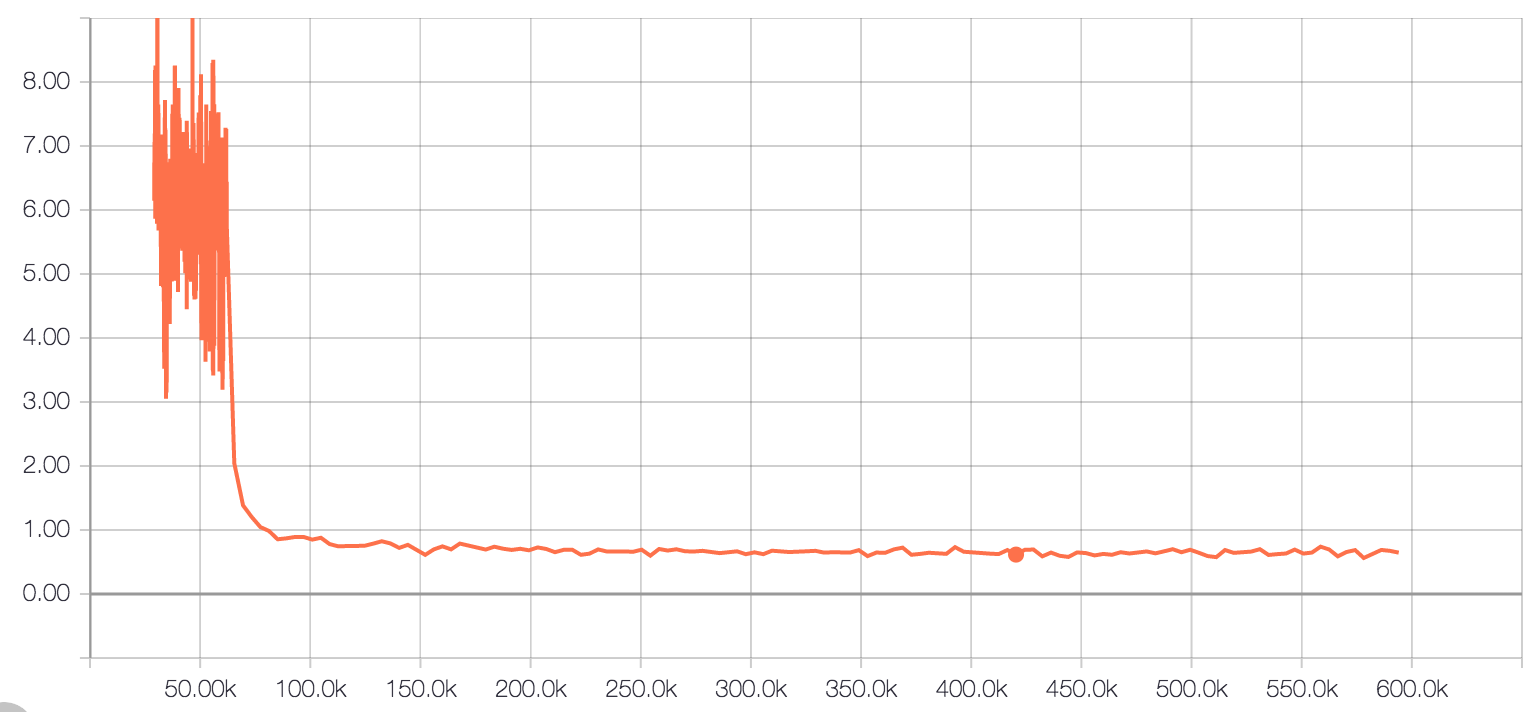
\includegraphics[width=\linewidth]{exp5-1}
  \caption{
    Función de error para el entrenamiento de la LSTM, dándole como estado inicial\
    un tensor generado a apartir de la red \emph{Inception V3} afinada.
    (Fuente: elaboración propia.)
  }
  \label{exp5}
\end{figure}

Para refinar el desempeño de la CNN afinada, el siguiente experimento se diseñó muestreando aleatoriamente\
\textbf{3416} personajes. Además, se eliminaron todas las palabras que no aparecen al menos\
5 veces en todo el conjunto de datos y se usaron únicamente 5 leyendas\
para cada personaje, con el fin de reducir el tamaño del vocabulario. Por consiguiente\
el vocabulario se redujo a 4528 palabras.\par
Previo al entrenamiento, se mezclaron los datos de manera aleatoria en el tensor $(I, S)$;\
esto provocó la diversificación en la manera con la que se generan leyendas para\
imágenes que no aparecen en el conjunto de entrenamiento. El comportamiento de la función de\
error se muestra en la Figura \ref{exp6}.

\begin{figure}[H]
  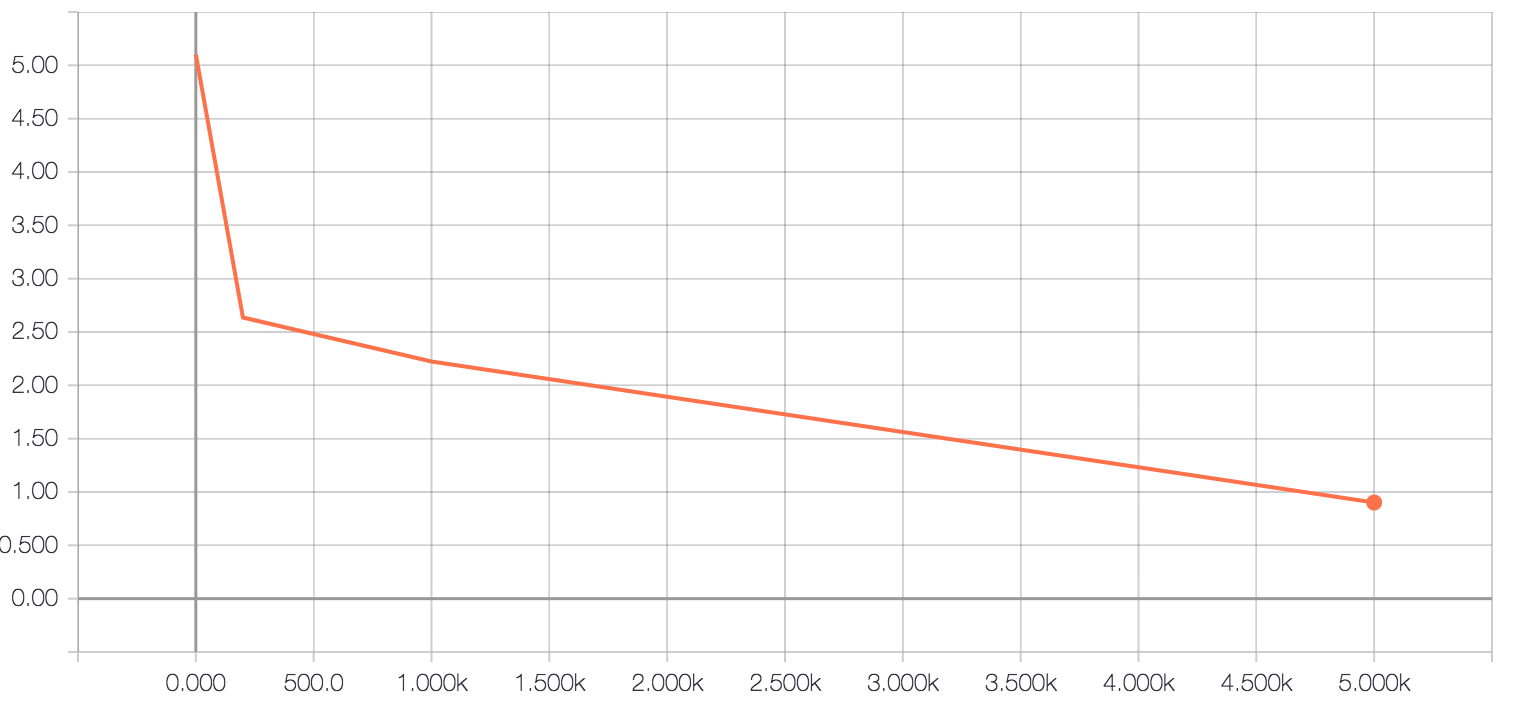
\includegraphics[width=\linewidth]{exp6-1}
  \caption{
    Función de error para el experimento que involucra la red \emph{Inception V3}
    afinada y 5 leyendas por personaje en el entrenamiento.
    (Fuente: elaboración propia.)
  }
  \label{exp6}
\end{figure}

Cualitativamente, la Figura \ref{exp6} muestra una curva descendente más suave, lo que hace pensar\
que el modelo, en efecto, aprendió a generalizar ciertos detalles del conjunto de datos. En promedio,\
podemos afirmar que el error de la entropía cruzada baja, con los cambios hechos y da cierto grado de\
confianza debido a la mezcla aleatoria de las leyendas. Por otro lado, queda la duda de qué pasaría si\
el tensor de códigos convolucionales es generado a partir de una CNN más superficial, algo que es\
válido plantearse debido al número de imágenes disponibles.\par
Este último experimento será el que mejor desempeño trae de los que usaron la red \emph{Inception V3}\
afinada. Efectuar métricas de evaluación como \emph{precisión} y \emph{error medio absoluto} es una\
práctica poco común en tareas que involucran generación de texto: la calidad de las leyendas generadas\
debe ser comparada con un modelo de lenguaje real. Por ello, en la Sección \ref{sec:metrics} presentamos\
una evaluación basada en una métrica común para el procesamiento del lenguaje natural. La Tabla\
\ref{exp6:anec} muestra algunos resultados anecdóticos de este experimento.

\subsection{Experimentos que involucran una arquitectura convolucional superficial}

\noindent
Aunque afinar una CNN profunda, previamente entrenada, es un procedimiento justificado por la literatura,\
el número máximo de imágenes que conforman el conjunto de datos sugiere otro tratamiento.\
Esto indica que entrenar una red neuronal desde cero no es una mala apuesta,\
después de todo, de acuerdo a \cite{DBLP:journals/corr/YosinskiCBL14}.\par
Ahora, presentamos el entrenamiento de una red neuronal superficial (\emph{bastante menos profunda}).\
Se usaron los mismos datos que para la afinación de \emph{Inception V3}.
La arquitectura de esta red se muestra en la Tabla \ref{capas-small},\
el desempeño del entrenamiento se ilustra en la Figura \ref{exp3}, mientras que\
la evaluación del modelo se encuentra en la Figura \ref{eval:exp3}.

\begin{table}[h]
  \resizebox{\textwidth}{!}{
    \begin{tabular}{|l|c|c|}
      \hline
      \textbf{tipo} & \textbf{tamaño de filtro} & \textbf{número de filtros}\\
      \hline \hline
      CONV & $3 \times 3$ & $32$ \\
      \hline
      CONV & $3 \times 3$ & $16$ \\
      \hline
      POOL & $2 \times 2$ & - \\
      \hline
      DROPOUT & $25\%$ de las neuronas se ignoran & - \\
      \hline
      MLP & $128$ unidades de salida & - \\
      \hline
      DROPOUT & $50\%$ de las neuronas se ignoran & - \\
      \hline
      MLP & $2$ unidades de salida & - \\
      \hline
    \end{tabular}
  }
  \caption[Nota al pie]{
    Arquitectura utilizada para entrenar una CNN superficial. Las capas
    \textbf{DROPOUT} constituyen una popular técnica de \emph{regularización}\footnotemark en
    la que se descarta un porcentaje dado de las neuronas de entrada con el fin
    de evitar un sobreajuste sobre el conjunto de datos en cuestión.
  }
  \label{capas-small}
\end{table}

\footnotetext{
  Las técnicas de \textbf{regularización}, en aprendizaje automático, añaden una
  restricción adicional al problema en cuestión para evitar que los valores
  del modelo propuesto se ajusten completamente al conjunto de datos de entrenamiento.
  Es decir, evitar el \emph{sobreajuste} y favorecer la generalización hacia datos
  no observados durante el entrenamiento.
}

\begin{figure}[H]
  \begin{minipage}[c]{\linewidth}
    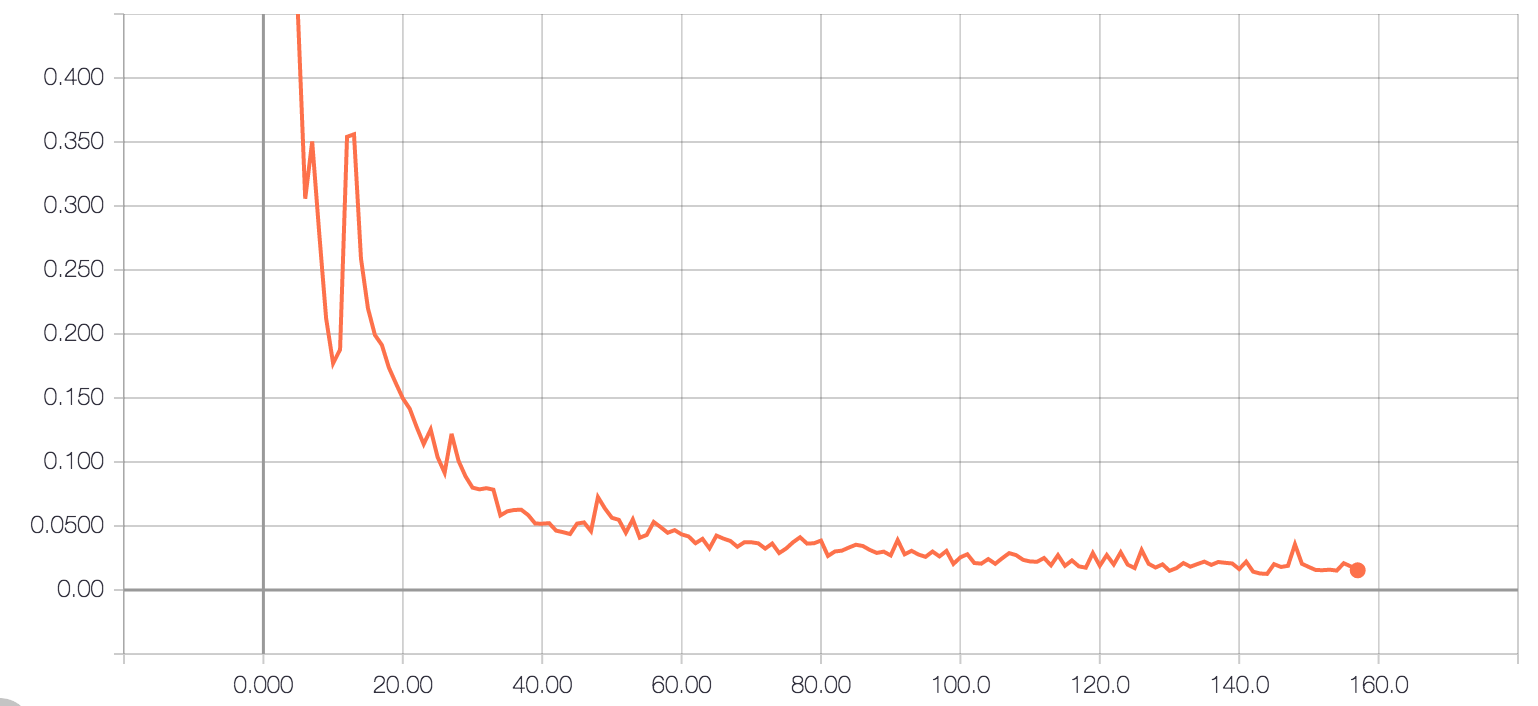
\includegraphics[width=\linewidth]{exp3-1}
  \end{minipage}\hfill
  \begin{minipage}[c]{\linewidth}
    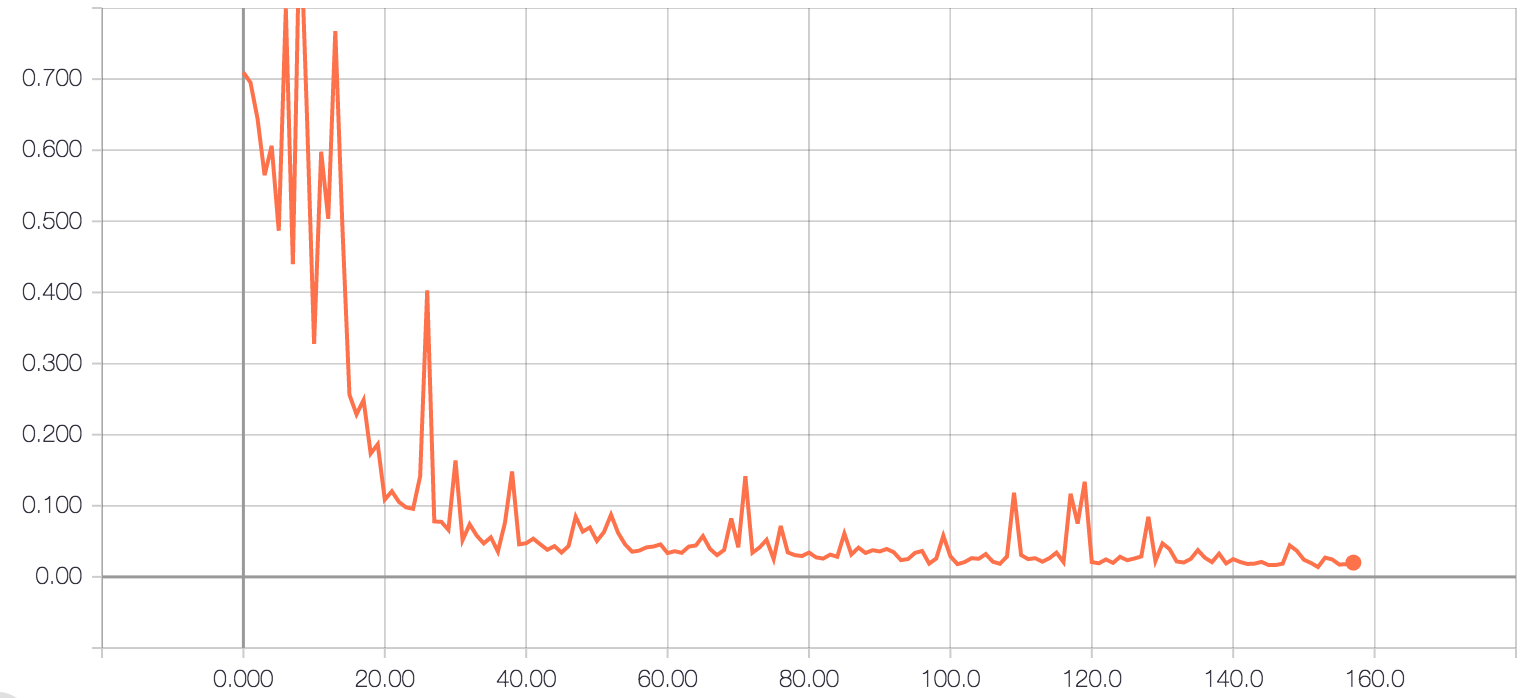
\includegraphics[width=\linewidth]{exp3-2}
  \end{minipage}
  \caption{
    Funciones de error de entrenamiento y validación (gráfico de arriba y de abajo,
    respectivamente) de la CNN superficial. Obsérvese que
    solo se requirieron alrededor de 150 épocas de entrenamiento para llegar a un
    valor óptimo; esto dado el tamaño del conjunto de datos (\emph{memes} y
    \emph{no memes}) que es bastantes órdenes de magnitud más pequeño el\
    conjunto de datos de entrenamiento presentado en la Sección \ref{sec:dataset}.
    (Fuente: elaboración propia.)
  }
  \label{exp3}
\end{figure}

Procedemos, entonces, a replicar el último experimento realizado en la sección anterior.\
Sin embargo, esta vez utilizamos la CNN superficial entrenada sobre memes y no memes.\
El entrenamiento arrojado (Figura \ref{exp7}) fue muy similar a lo observado en la\
Figura \ref{exp6}; no obstante, se logró una mejora en la calidad de las leyendas\
sin ser un detalle anecdótico muy considerable (Tabla \ref{exp7:anec}).

\begin{figure}[H]
  \centering
  \begin{minipage}[c]{\linewidth}
    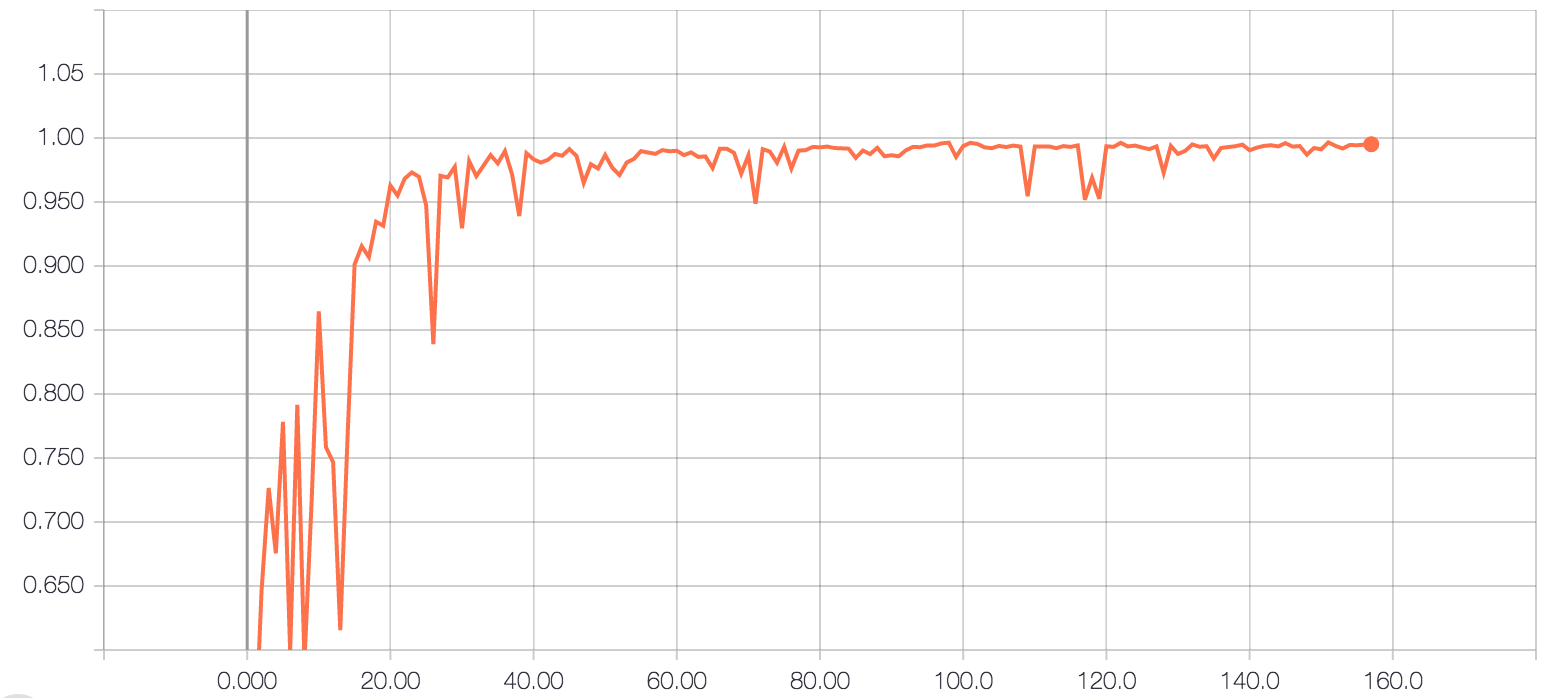
\includegraphics[width=\linewidth]{exp3-3}
  \end{minipage}\hfill
  \begin{minipage}[c]{\linewidth}
    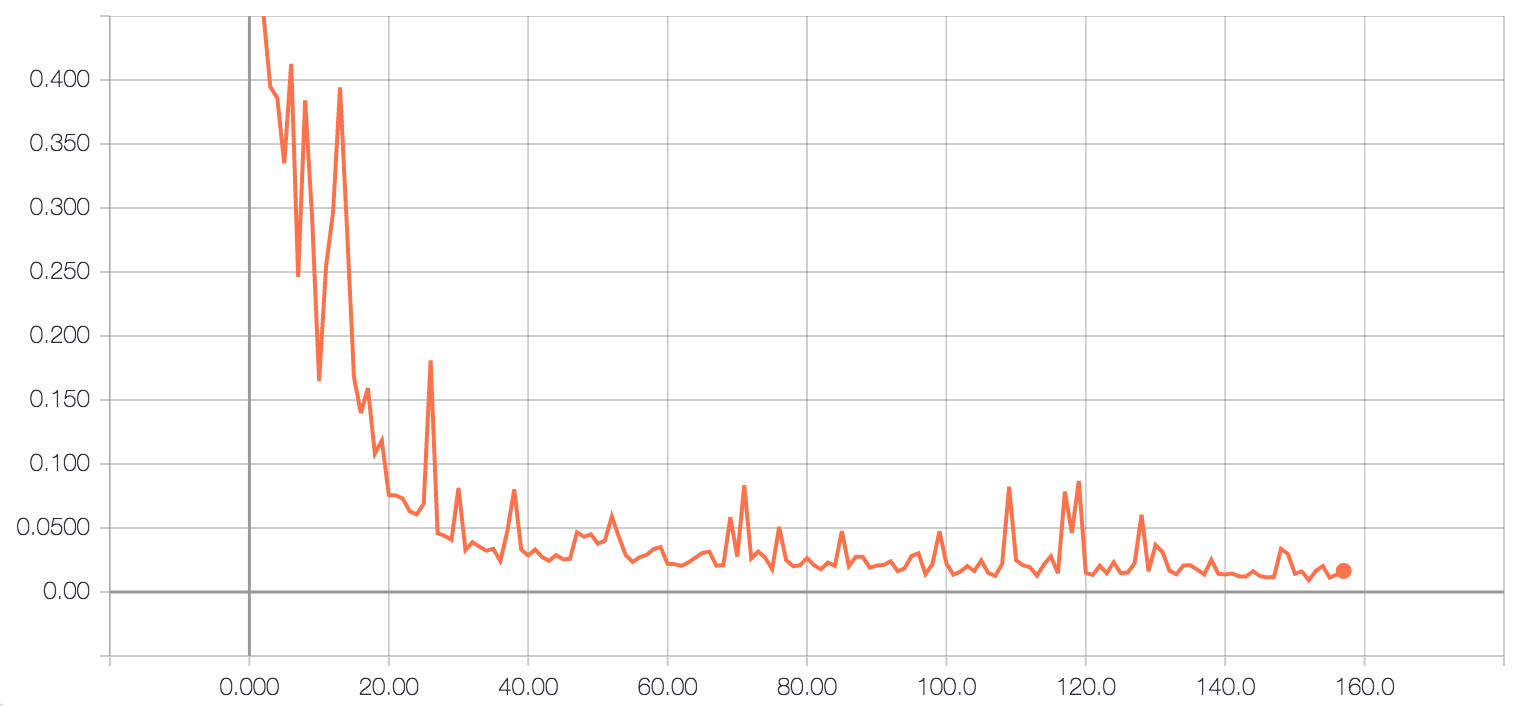
\includegraphics[width=\linewidth]{exp3-4}
  \end{minipage}
  \caption{
    Dos funciones de evaluación para el modelo convolucional superficial.
    El gráfico de la parte superior muestra la \emph{precisión} con la que el modelo realiza
    sus clasificaciones, mientras que el gráfico de la parte inferior muestra el
    \emph{error medio absoluto} entre las clasificaciones hechas modelo contra las verdaderas.
    Ambos gráficos se generaron a partir de un muestreo del $10\%$ de los datos disponibles.
    (Fuente: elaboración propia.)
  }
  \label{eval:exp3}
\end{figure}

Hasta este punto, podemos decir que hemos construido dos modelos convolucionales capaces\
de distinguir entre cualesquiera dos personajes. La tarea pendiente recae en hallar los\
(\emph{híper})-parámetros necesarios para que las leyendas generadas tengan más sentido a juicio\
de un ser humano. Por ello, reportamos un último experimento que involucra un mayor número de palabras\
por personaje.

\begin{figure}[H]
  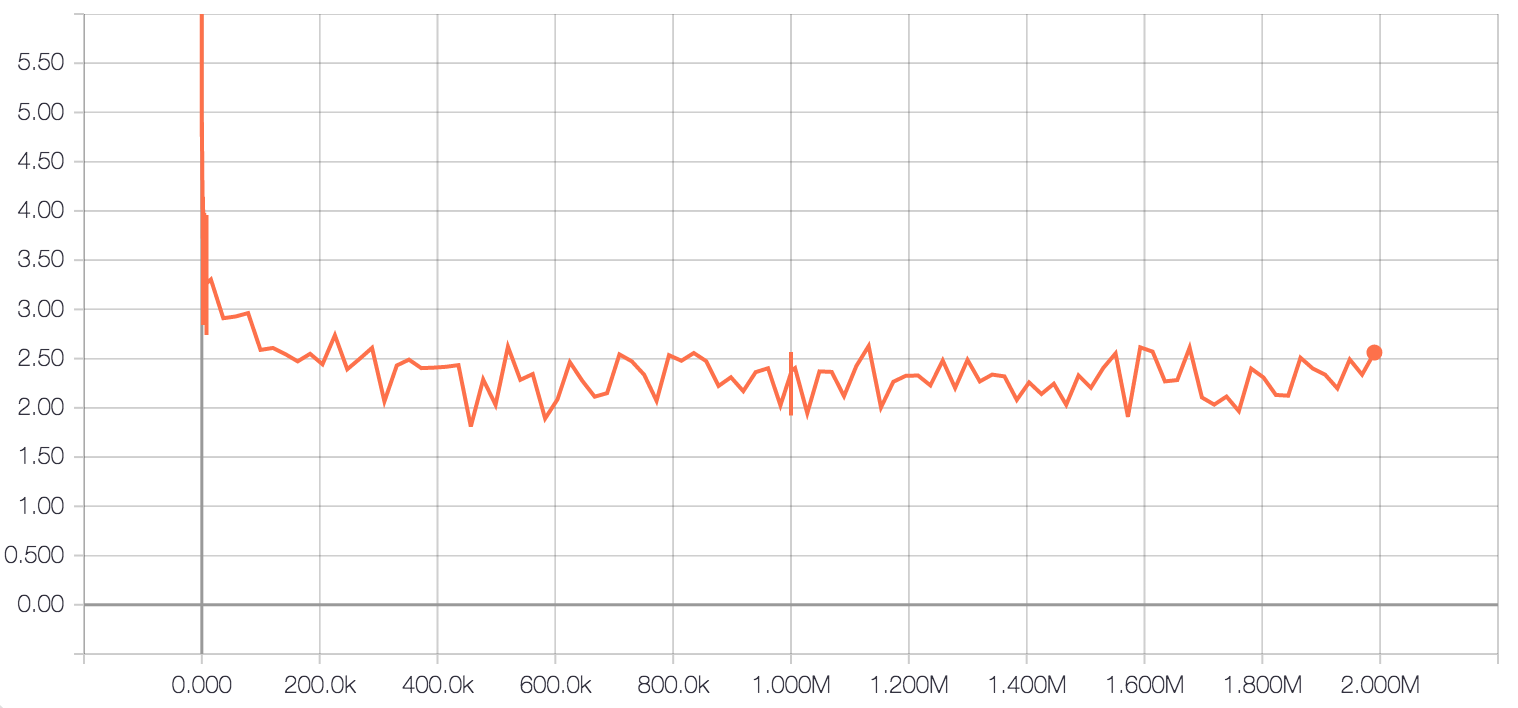
\includegraphics[width=\linewidth]{exp7-1}
  \caption{
    Función de error para el entrenamiento de la LSTM, usando 5 leyendas por personaje,
    un vocabulario reducido y códigos convolucionales generados a partir de una CNN superficial.
    (Fuente: elaboración propia.)
  }
  \label{exp7}
\end{figure}

\begin{figure}[H]
  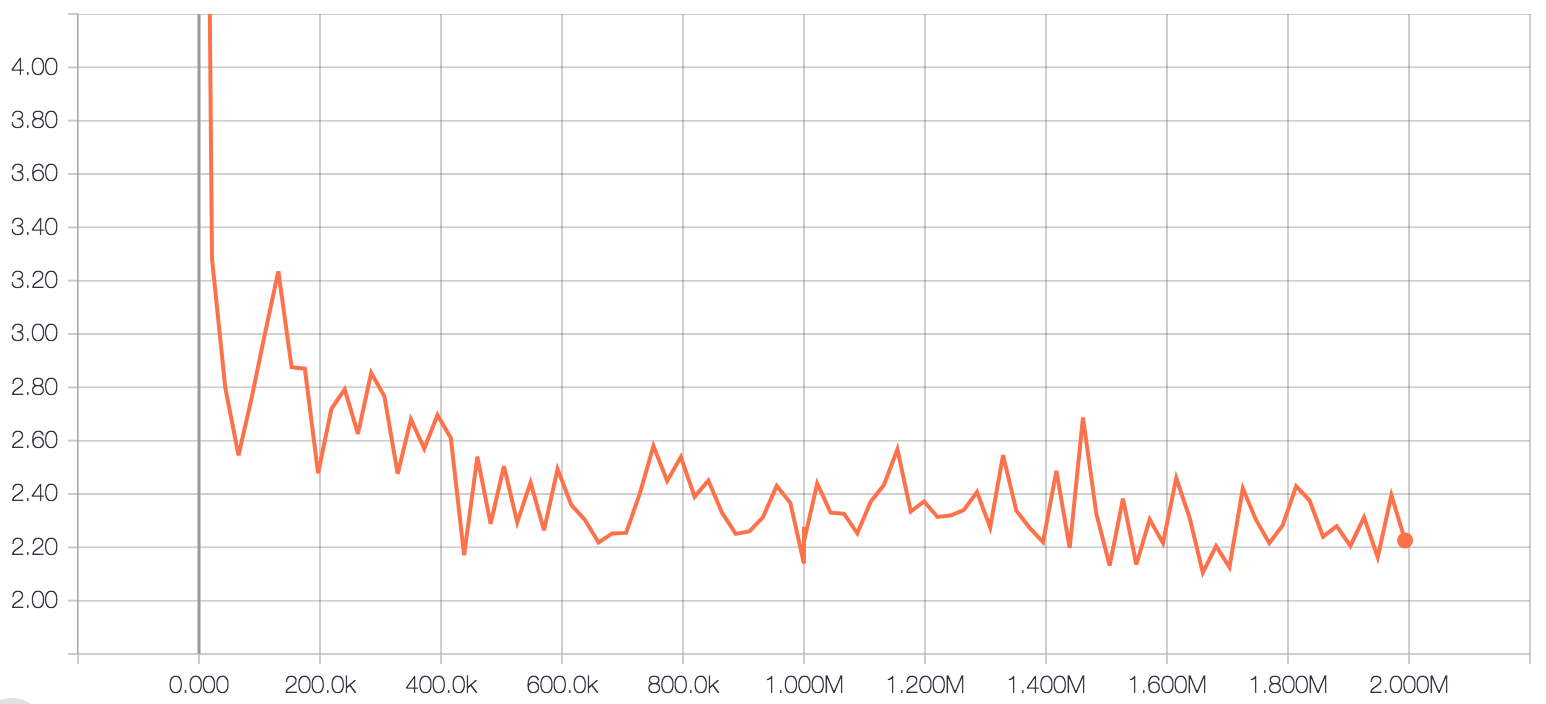
\includegraphics[width=\linewidth]{exp8-1}
  \caption{
    Función de error para el entrenamiento de la LSTM, con códigos convolucionales dados
    por una CNN superficial y 20 leyendas por imagen. Como se observa, existe una ligera
    disminución en el error resultante al final del entrenamiento, con respecto al obtenido
    en experimentos anteriores.
    (Fuente: elaboración propia.)
  }
  \label{exp8}
\end{figure}

Con los mismos datos que para el experimento anterior y con la CNN superficial, se realizó\
el entrenamiento cuyo desempeño se ilustra en la Figura \ref{exp8}. Ahora se aumentó a 20 el\
número de leyendas por imagen. En cuanto a detalles anecdóticos, la Tabla \ref{exp8:anec}\
ilustra una generación de leyendas con un poco de más sentido cuando hay dos palabras\
distintas contiguas. Resumimos los detalles técnicos de todos los experimentos presentados\
en la Tabla \ref{exp-details}.

\begin{table}[H]
  \begin{tabular}{|p{0.5\linewidth}|p{0.2\linewidth}|p{0.3\linewidth}|}
    \hline
    \textbf{tipo de experimento} & \textbf{número de personajes} & \textbf{número de leyendas por personaje}\\
    \hline \hline
    Réplica de entrenamiento de \emph{Inception V3}, como en \cite{DBLP:journals/corr/VinyalsTBE16} & \multicolumn{2}{|c|}{Conjunto de datos \emph{ImageNet}} \\
    \hline
    LSTM a partir de \emph{Inception V3} & 97 & 700, en promedio \\
    \hline
    Afinación de \emph{Inception V3} & \multicolumn{2}{|c|}{3065 memes y 3065 no memes} \\
    \hline
    LSTM a partir de \emph{Inception V3} afinada & 97 & 700, en promedio \\
    \hline
    LSTM a partir de \emph{Inception V3} afinada & 3416 & 5 \\
    \hline
    Entrenamiento de una CNN superficial & \multicolumn{2}{|c|}{3065 memes y 3065 no memes} \\
    \hline
    LSTM a partir de la CNN superficial & 3416 & 5 \\
    \hline
    LSTM a partir de la CNN superficial & 3416 & 20 \\
    \hline
  \end{tabular}
  \caption{
    Resumen de los detalles técnicos presentados en esta sección.
  }
  \label{exp-details}
\end{table}

\section{Evaluación del desempeño de la LSTM} \label{sec:metrics}

\noindent
En el contexto del procesamiento del lenguaje natural, es común preguntarse qué tan \emph{buenos}\
son los enunciados generados con respecto a un lenguaje referencia. En el caso que concierne a esta tesis,\
tratamos con un lenguaje informal, generado a partir de la popularidad que adquieren ciertas frases\
dentro del Internet. Sin embargo, es posible discernir entre un enunciado que hace sentido\
empírico a uno que combina palabras sin patrón alguno.\par
Las métricas propuestas en \cite{DBLP:journals/corr/VinyalsTBE16} sugieren el uso de un corpus\
lingüístico de referencia, con el cual se compare la similitud entre las estructuras gramaticales\
generadas por el modelo con enunciados ``reales''. Por ello, hemos construido un corpus lingüístico
formado por leyendas en el conjunto de \emph{evaluación} para fines de realizar una comparación\
con los resultados emitidos por la LSTM.\par
En particular, analizamos qué tan bien aprende el modelo a predecir la $t$-ésima palabra, a nivel\
probabilístico. Dada la distribución de probabilidad $p$ sobre los enunciados realizados a partir\
de un alfabeto $\Sigma$%
\footnote{
  Es decir, un modelo de lenguaje.
}, definimos la \textbf{perplejidad} $PP(S)$ del modelo como
\begin{equation}
  PP(S) = p(s_1 s_2 \ldots s_n) ^{-\frac{1}{n}}, \label{eq:perplexity0}
\end{equation}
donde $S = s_1, s_2, \ldots, s_n \in S^*$. Desarrollando la Ecuación \ref{eq:perplexity0},\
tenemos que
\begin{align}
  PP(S) &= \sqrt[n]{\frac{1}{p(s_1 s_2 \ldots s_n)}}\\
  &= \sqrt[n]{\prod_{i=0}^n \frac{1}{p(s_{i+1}\ |\ s_1 s_2 \ldots s_i)}} \label{eq:perplexity1}
\end{align}\par
La Ecuación \ref{eq:perplexity1} se obtuvo aplicando la \emph{regla de la cadena} de las probabilidades\
conjuntas a la predicción de cada palabra $s_i$. Lo que este razonamiento nos indica es que\
minimizar la perplejidad de un enunciado $S$ con respecto a un modelo $p$, es lo mismo que\
maximizar la probabilidad de $S$ bajo $p$.\par
Intuitivamente, la \emph{perplejidad} del modelo nos dice el número de posibles candidatos que tiene\
el modelo para la palabra $s_{i+1}$, dadas $s_1, s_2, \ldots, s_i$. Si la \emph{perplejidad} es minimizada,\
entonces el modelo aprende con éxito a descubrir patrones de secuencias de palabras.\par
Queremos comparar los dos \emph{mejores} modelos entrenados, es decir, el mejor de los que\
codifican imágenes con la arquitectura convolucional superficial contra el mejor de los que\
codifican con \emph{Inception V3}. Llamémoslos \verb+Modelo A+ y \verb+Modelo B+, respectivamente.\
Para exponerlos a un conjunto de imágenes ajenas a los datos de entrenamiento, se tomaron 20 ``nuevos\
memes'' (la mayoría, provenientes de sitios web con gran popularidad actual%
\footnote{
  \url{https://www.reddit.com} y \url{https://me.me}.
}), 20 de las imágenes del conjunto de datos de evaluación\
y 20 imágenes nuevas de \emph{ImageNet} (``no memes''). Esta distinción se hizo con el fin de mostrar\
qué tanto aprendió el modelo acerca de los memes y qué tanto generalizó en detalles.\par
Los promedios de las perplejidades arrojadas por cada experimento de\
evaluación se muestran en la Tabla \ref{avgperplexities}. Observamos que la profundidad de la\
CNN del \verb+Modelo B+ brinda un mejor contexto a la LSTM de los\
atributos que constituyen a la imagen de entrada, por lo que se justifica la discrepancia entre las\
perplejidades del \verb+Modelo A+ y del \verb+Modelo B+.\par
Recordemos que la CNN del \verb+Modelo A+ fue entrenada bajo la tarea de distinguir el conjunto de datos\
de memes con un subconjunto de \emph{ImageNet}. Por ello, muchas abstracciones posiblemente identificadas\
por la CNN del \verb+Modelo B+ no logran ser reflejadas en las salidas de la CNN del \verb+Modelo A+.\
Más aún, como la CNN del \verb+Modelo B+ estuvo previamente entrenada con los datos de \emph{ImageNet},\
de los cuales surgen los ``no memes'', es entendible que dicho modelo haya logrado un desempeño similar con\
``no memes'' y memes de evaluación. En contraste, los nuevos memes constituyen una clase de imágenes que no\
fue parte tanto del pre-entrenamiento como de la afinación del \verb+Modelo B+.\par
Los resultados de la evaluación pueden ser consultados de manera\
interactiva en el \textbf{repositorio de código fuente}%
\footnote{
  El repositorio se encuentra en \url{https://github.com/alorozco53/Deep-Meme-Captioner/blob/evaluate/memes/testing.md}.
} de esta tesis.

\begin{table}[H]
  \centering
  \includegraphics[width=\textwidth]{avgperplexities}
  \caption{
    Promedios de las perplejidades arrojadas al evaluar los dos \emph{mejores} modelos contra el
    \emph{corpus} formado mediante las leyendas de los memes extraídos de Internet.
  }
  \label{avgperplexities}
\end{table}

\chapter{Conclusiones}

TODO


%% \bibliographystyle{acm}
%% \bibliography{bibliography} 
\printbibliography

\appendix

\backmatter

\end{document}
